\pagebreak
\subsection{Native coordinates NetCDF GRID\_GEOMETRY\_ECCO}
\newp
\begin{longtable}{|p{0.1\textwidth}|p{0.5\textwidth}|}
    \caption{Variables in the dataset GRID\_GEOMETRY\_ECCO}
    \label{tab:table-GRID_GEOMETRY_ECCO-fields} \\ 
    \hline \endhead \hline \endfoot
    \rowcolor{lightgray} \textbf{Dataset:} & \textbf{GRID\_GEOMETRY\_ECCO} \\ \hline
    Field: &XC \\ \hline
    Field: &YC \\ \hline
    Field: &XG \\ \hline
    Field: &YG \\ \hline
    Field: &CS \\ \hline
    Field: &SN \\ \hline
    Field: &rA \\ \hline
    Field: &dxG \\ \hline
    Field: &dyG \\ \hline
    Field: &Depth \\ \hline
    Field: &rAz \\ \hline
    Field: &dxC \\ \hline
    Field: &dyC \\ \hline
    Field: &rAw \\ \hline
    Field: &rAs \\ \hline
    Field: &hFacC \\ \hline
    Field: &hFacW \\ \hline
    Field: &hFacS \\ \hline
    Field: &maskC \\ \hline
    Field: &maskW \\ \hline
    Field: &maskS \\ \hline
\end{longtable}

\pagebreak
\subsubsection{Native coordinates Variable XC}
\begin{longtable}{|p{0.06\textwidth}|p{0.41\textwidth}|p{0.39\textwidth}|p{0.06\textwidth}|}
    \caption{CDL description of GRID\_GEOMETRY\_ECCO's XC variable}
    \label{tab:table-GRID_GEOMETRY_ECCO_XC} \\ 
    \hline \endhead \hline \endfoot
    \rowcolor{lightgray} \textbf{Storage Type} & \textbf{Variable Name} & \textbf{Description} & \textbf{Unit} \\ \hline
    float32 & XC & longitude of tracer grid cell center & degrees\_east \\ \hline
    \rowcolor{lightgray}  \multicolumn{4}{|p{1.00\textwidth}|}{\textbf{CDL Description}} \\ \hline
    \multicolumn{4}{|p{1.00\textwidth}|}{\makecell{\parbox{1\textwidth}{float32 XC(tile, j, i)\\
    \hspace*{0.5cm}XC: long\_name = longitude of tracer grid cell center\\
    \hspace*{0.5cm}XC: units = degrees\_east\\
    \hspace*{0.5cm}XC: coordinate = YC\hspace*{0.5cm} XC\\
    \hspace*{0.5cm}XC: bounds =\hspace*{0.5cm} XC\_bnds\\
    \hspace*{0.5cm}XC: coverage\_content\_type = coordinate\\
    \hspace*{0.5cm}XC: standard\_name = longitude}}} \\ \hline
    \rowcolor{lightgray} \multicolumn{4}{|p{1.00\textwidth}|}{\textbf{Comments}} \\ \hline
    \multicolumn{4}{|p{1\textwidth}|}{nonuniform grid spacing} \\ \hline
\end{longtable}

\begin{figure}[H]
\centering
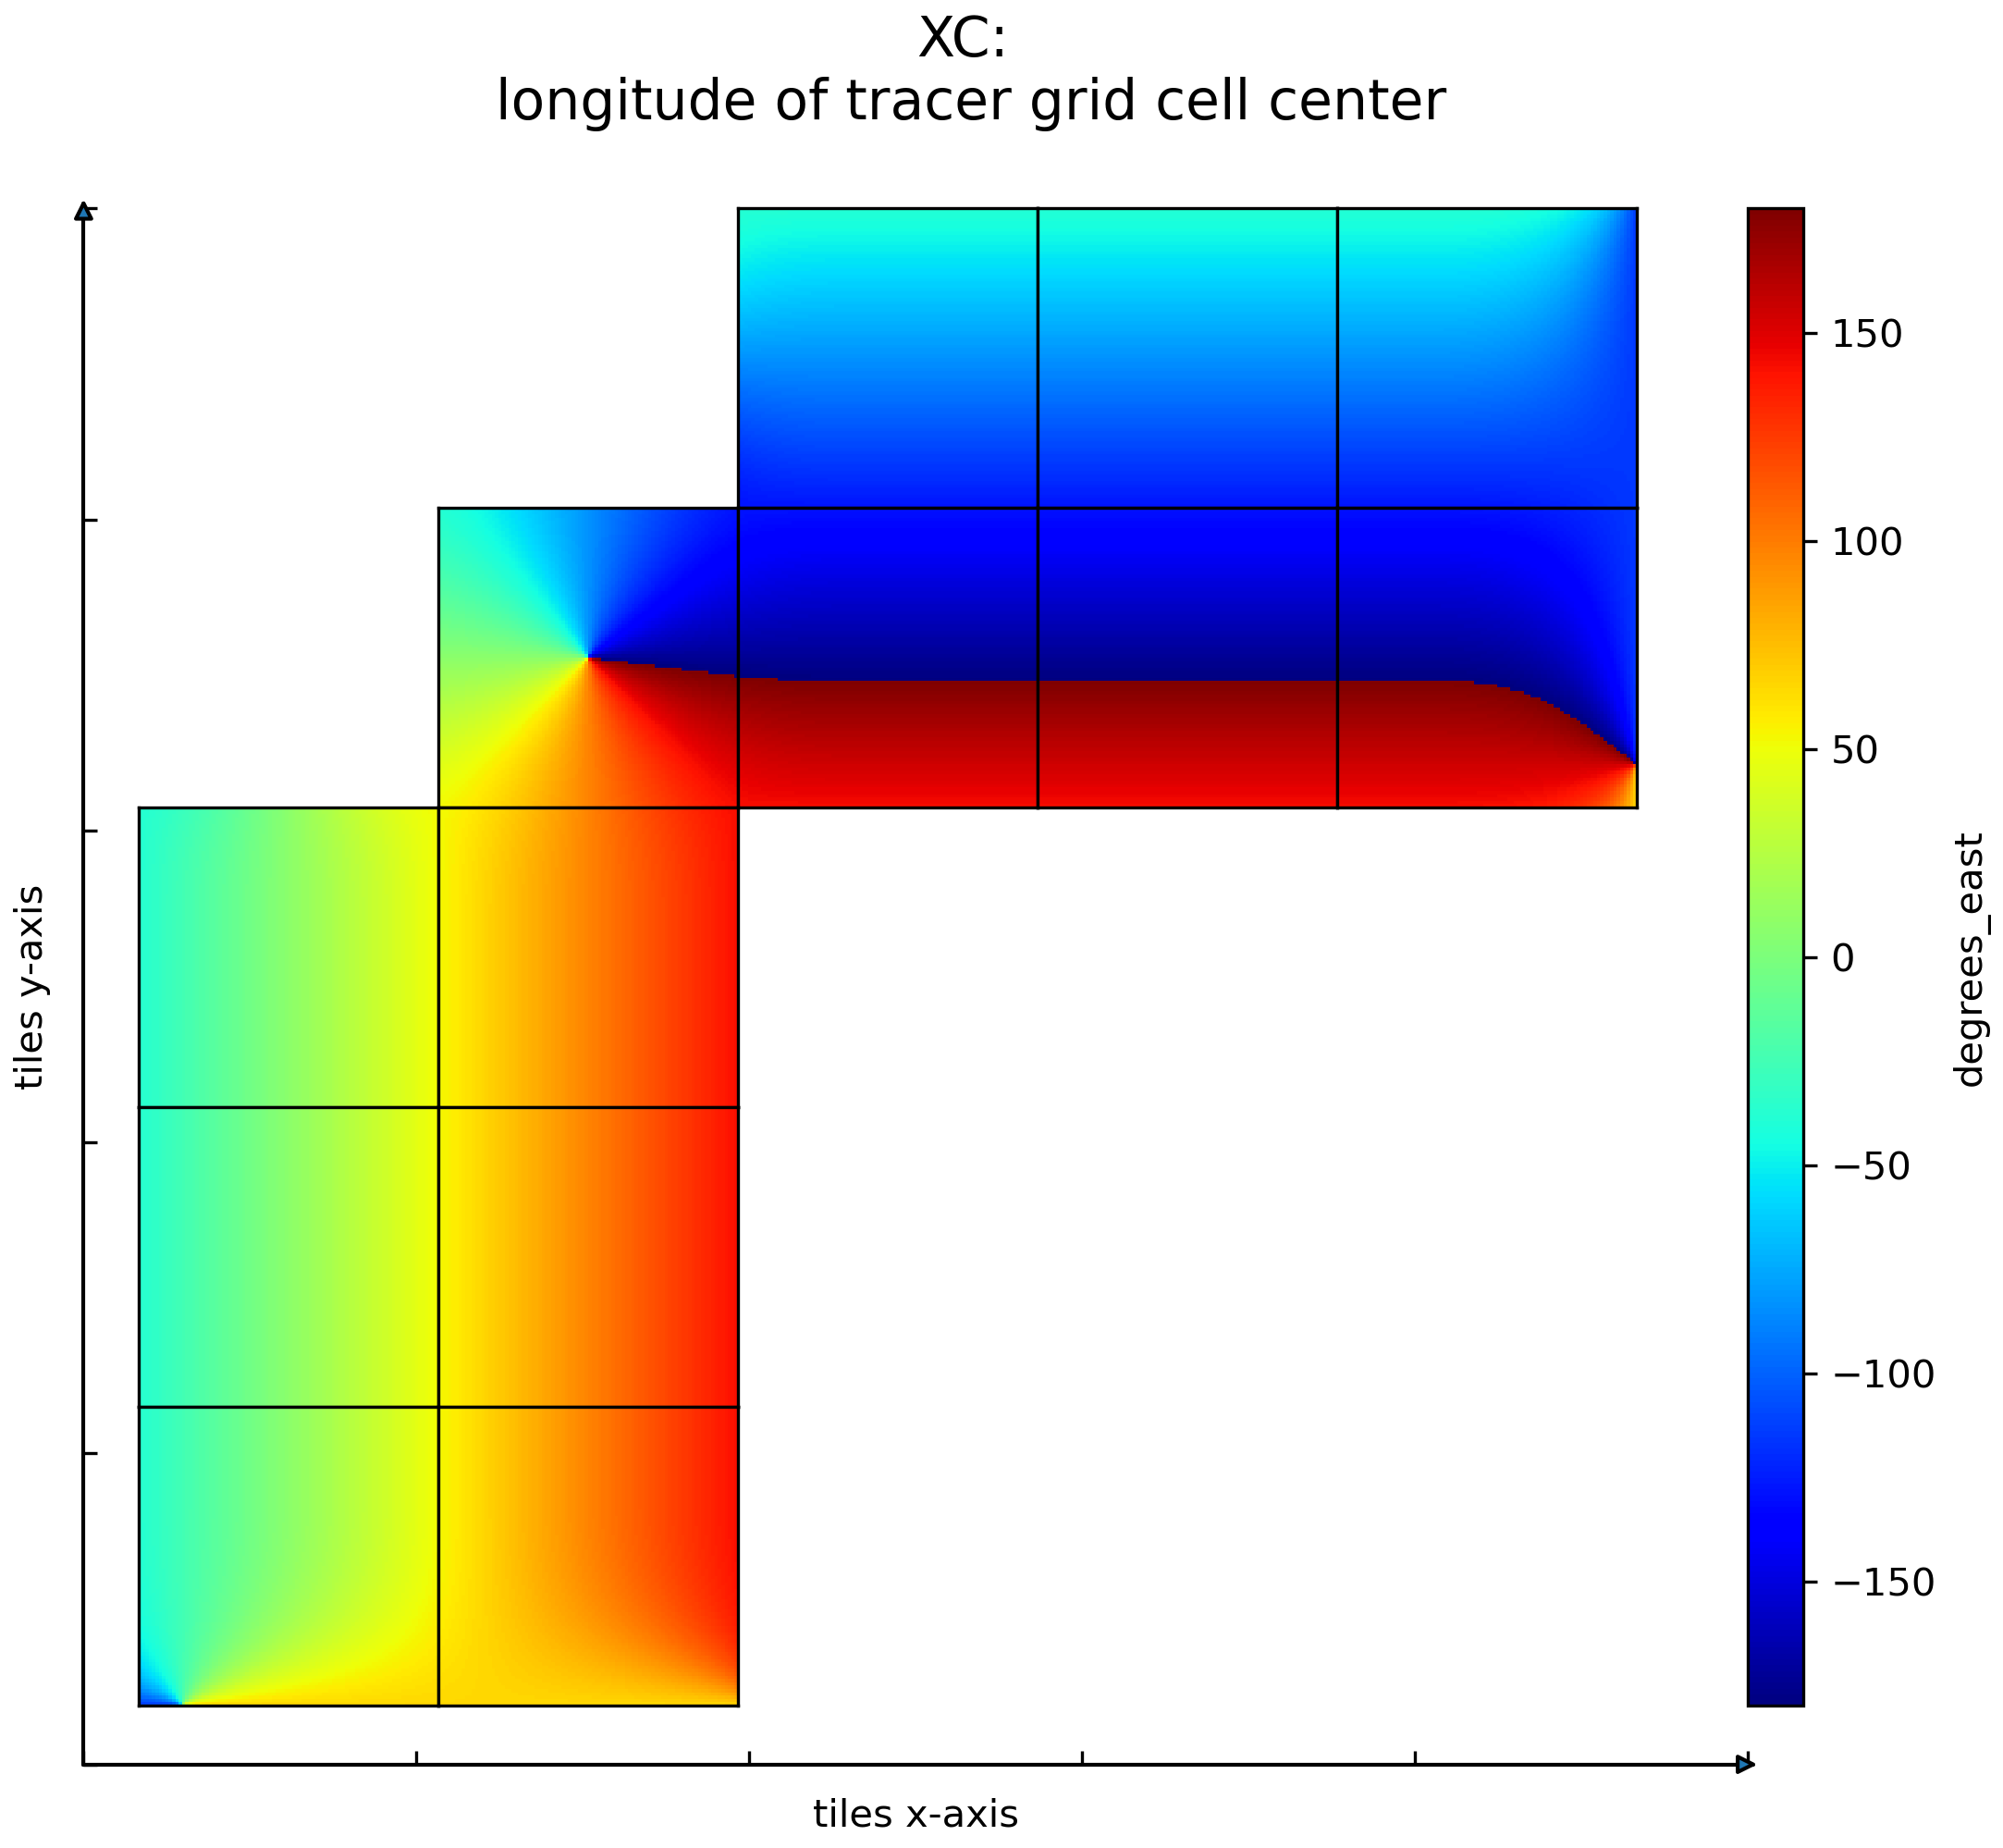
\includegraphics[scale=0.5]{../images/plots/native_plots_coords/Geometry_Parameters_for_the_Lat-Lon-Cap_90_(llc90)_Native_Model_Grid_(Version_4_Release_4)/XC.png}
\caption{\\Dataset: GRID\_GEOMETRY\_ECCO\\Variable: XC}
\label{tab:table-GRID_GEOMETRY_ECCO_XC-Plot}
\end{figure}
\pagebreak
\subsubsection{Native coordinates Variable YC}
\begin{longtable}{|p{0.06\textwidth}|p{0.41\textwidth}|p{0.39\textwidth}|p{0.06\textwidth}|}
    \caption{CDL description of GRID\_GEOMETRY\_ECCO's YC variable}
    \label{tab:table-GRID_GEOMETRY_ECCO_YC} \\ 
    \hline \endhead \hline \endfoot
    \rowcolor{lightgray} \textbf{Storage Type} & \textbf{Variable Name} & \textbf{Description} & \textbf{Unit} \\ \hline
    float32 & YC & latitude of tracer grid cell center & degrees\_north \\ \hline
    \rowcolor{lightgray}  \multicolumn{4}{|p{1.00\textwidth}|}{\textbf{CDL Description}} \\ \hline
    \multicolumn{4}{|p{1.00\textwidth}|}{\makecell{\parbox{1\textwidth}{float32 YC(tile, j, i)\\
    \hspace*{0.5cm}YC: long\_name = latitude of tracer grid cell center\\
    \hspace*{0.5cm}YC: units = degrees\_north\\
    \hspace*{0.5cm}YC: coordinate =\hspace*{0.5cm} YC XC\\
    \hspace*{0.5cm}YC: bounds =\hspace*{0.5cm} YC\_bnds\\
    \hspace*{0.5cm}YC: coverage\_content\_type = coordinate\\
    \hspace*{0.5cm}YC: standard\_name = latitude}}} \\ \hline
    \rowcolor{lightgray} \multicolumn{4}{|p{1.00\textwidth}|}{\textbf{Comments}} \\ \hline
    \multicolumn{4}{|p{1\textwidth}|}{nonuniform grid spacing} \\ \hline
\end{longtable}

\begin{figure}[H]
\centering
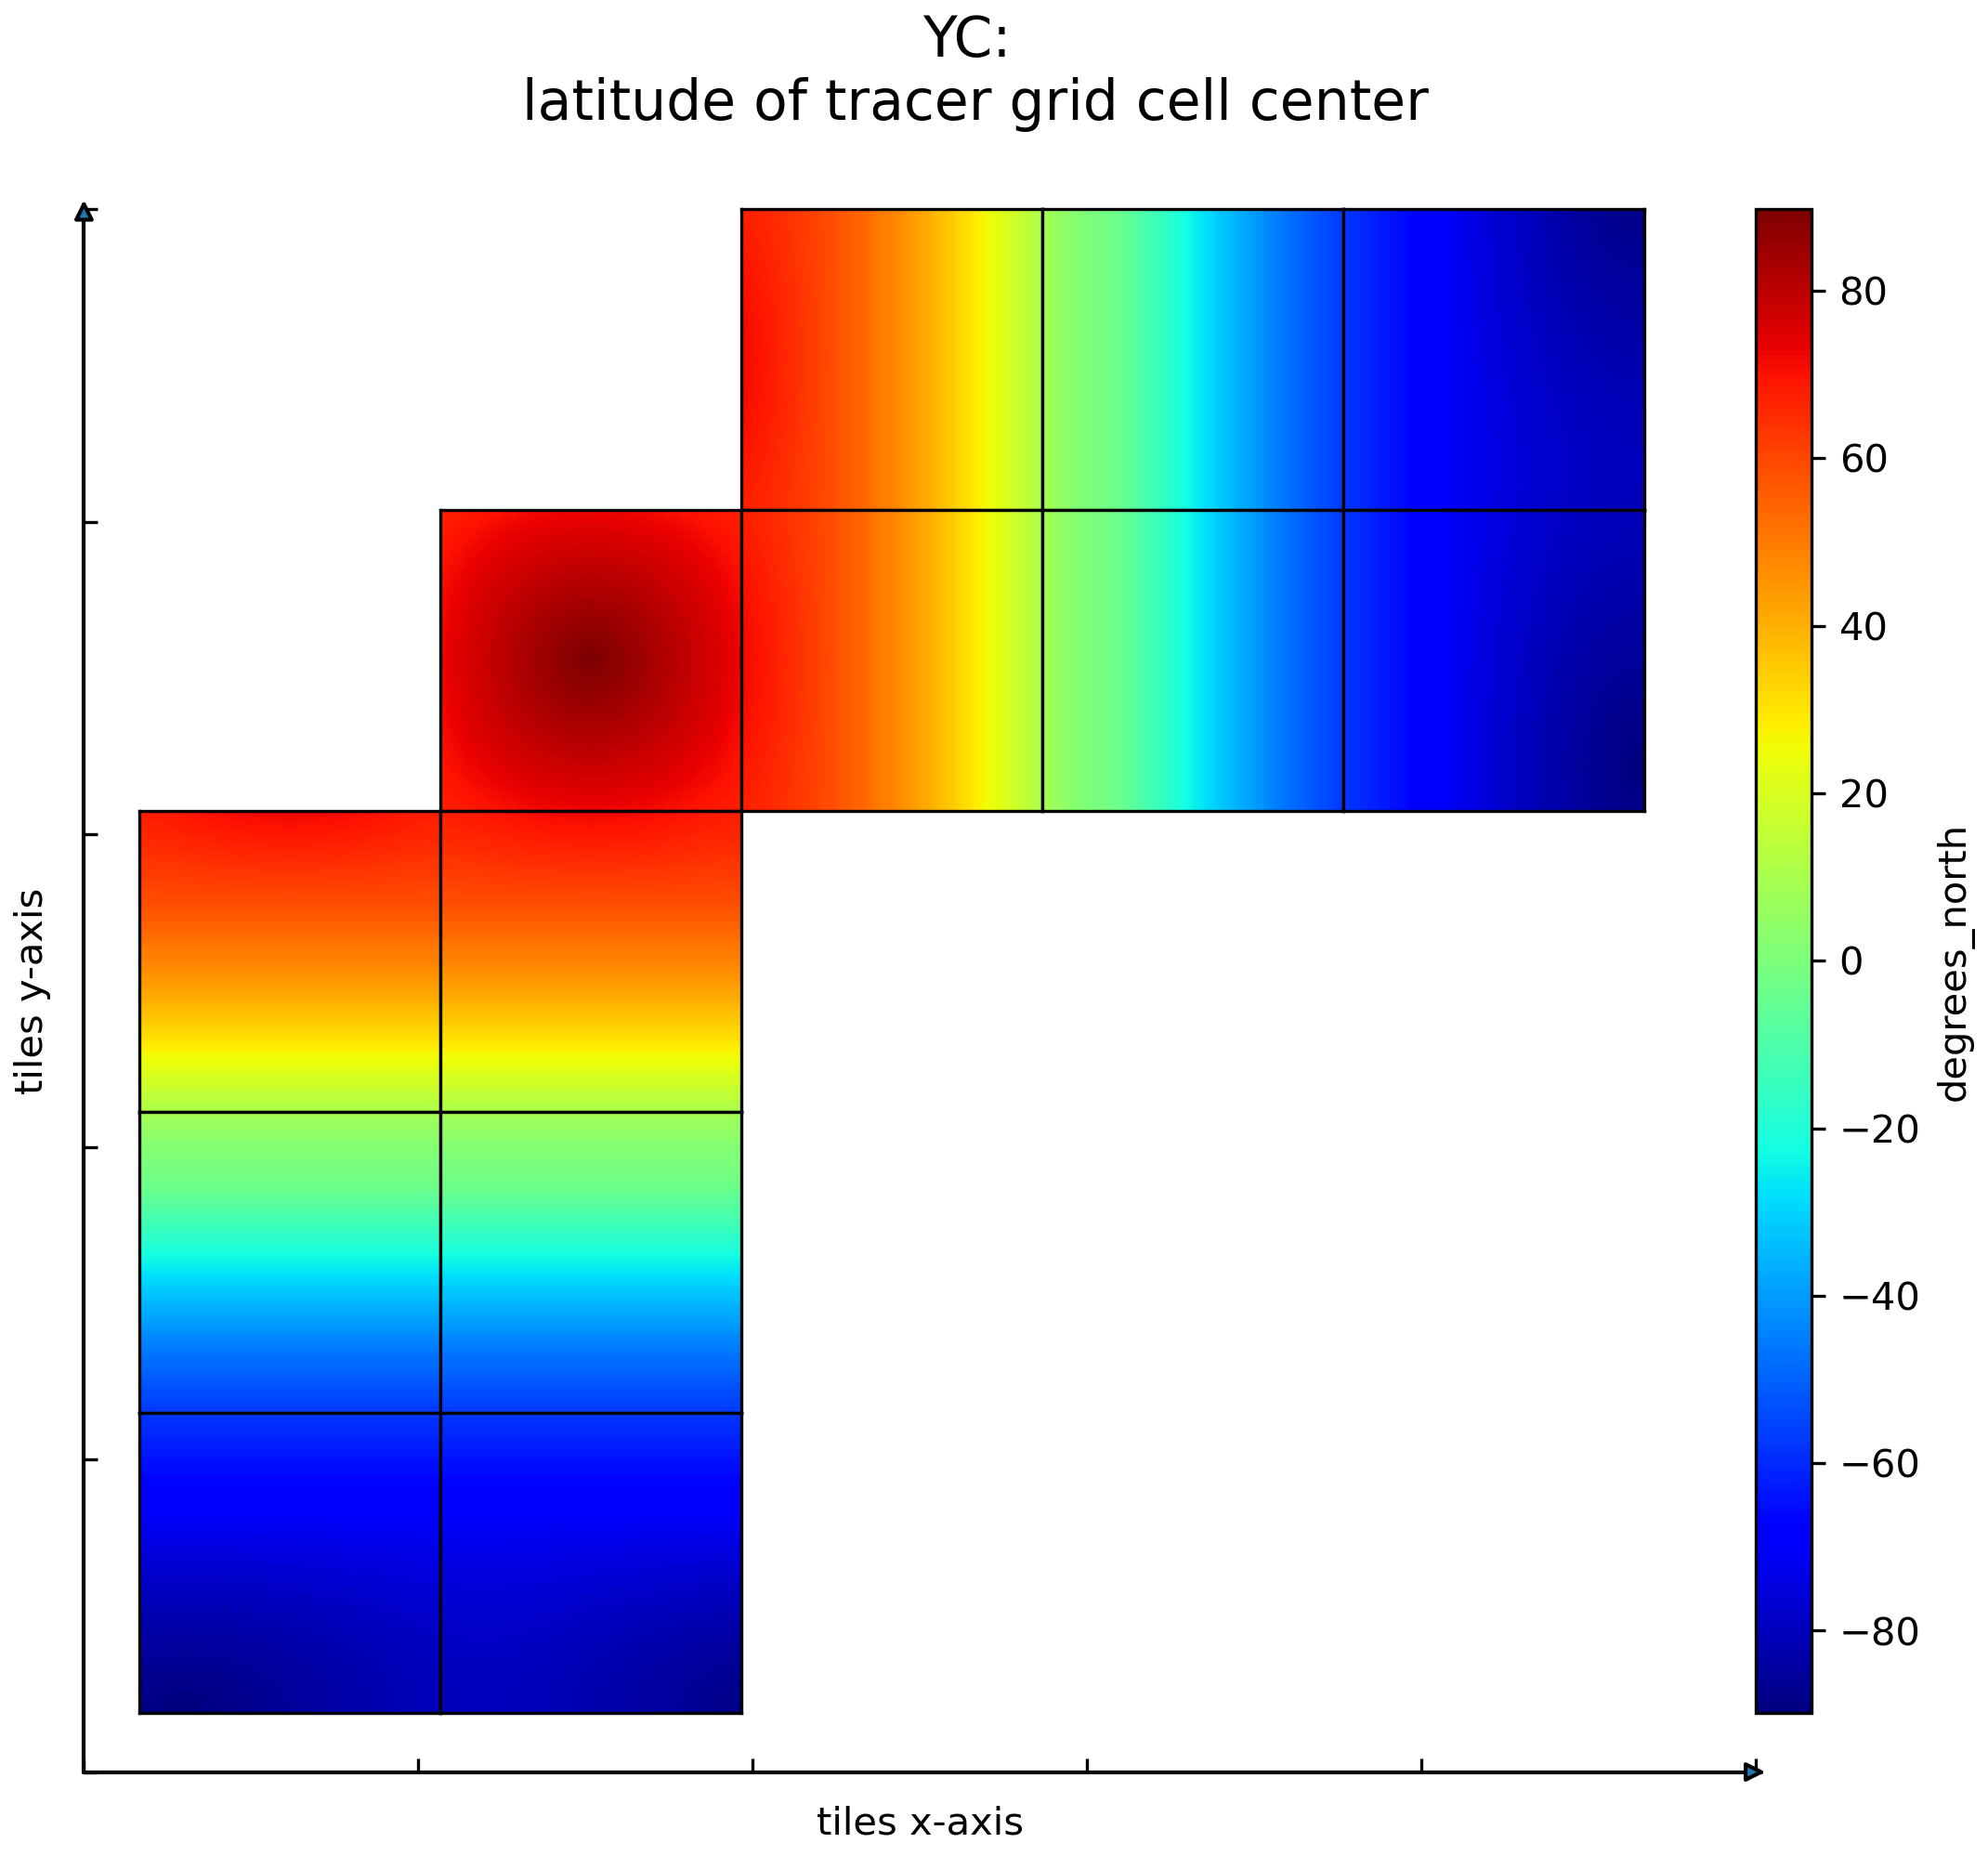
\includegraphics[scale=0.5]{../images/plots/native_plots_coords/Geometry_Parameters_for_the_Lat-Lon-Cap_90_(llc90)_Native_Model_Grid_(Version_4_Release_4)/YC.png}
\caption{\\Dataset: GRID\_GEOMETRY\_ECCO\\Variable: YC}
\label{tab:table-GRID_GEOMETRY_ECCO_YC-Plot}
\end{figure}
\pagebreak
\subsubsection{Native coordinates Variable XG}
\begin{longtable}{|p{0.06\textwidth}|p{0.41\textwidth}|p{0.39\textwidth}|p{0.06\textwidth}|}
    \caption{CDL description of GRID\_GEOMETRY\_ECCO's XG variable}
    \label{tab:table-GRID_GEOMETRY_ECCO_XG} \\ 
    \hline \endhead \hline \endfoot
    \rowcolor{lightgray} \textbf{Storage Type} & \textbf{Variable Name} & \textbf{Description} & \textbf{Unit} \\ \hline
    float32 & XG & longitude of 'southwest' corner of tracer grid cell & degrees\_east \\ \hline
    \rowcolor{lightgray}  \multicolumn{4}{|p{1.00\textwidth}|}{\textbf{CDL Description}} \\ \hline
    \multicolumn{4}{|p{1.00\textwidth}|}{\makecell{\parbox{1\textwidth}{float32 XG(tile, j\_g, i\_g)\\
    \hspace*{0.5cm}XG: long\_name = "longitude of southwest corner of tracer grid cell"\\
    \hspace*{0.5cm}XG: units = degrees\_east\\
    \hspace*{0.5cm}XG: coordinate = YG\hspace*{0.5cm} XG\\
    \hspace*{0.5cm}XG: coverage\_content\_type = coordinate\\
    \hspace*{0.5cm}XG: standard\_name = longitude}}} \\ \hline
    \rowcolor{lightgray} \multicolumn{4}{|p{1.00\textwidth}|}{\textbf{Comments}} \\ \hline
    \multicolumn{4}{|p{1\textwidth}|}{Nonuniform grid spacing. Note: 'southwest' does not correspond to geographic orientation but is used for convenience to describe the computational grid. See MITgcm dcoumentation for details.} \\ \hline
\end{longtable}

\begin{figure}[H]
\centering
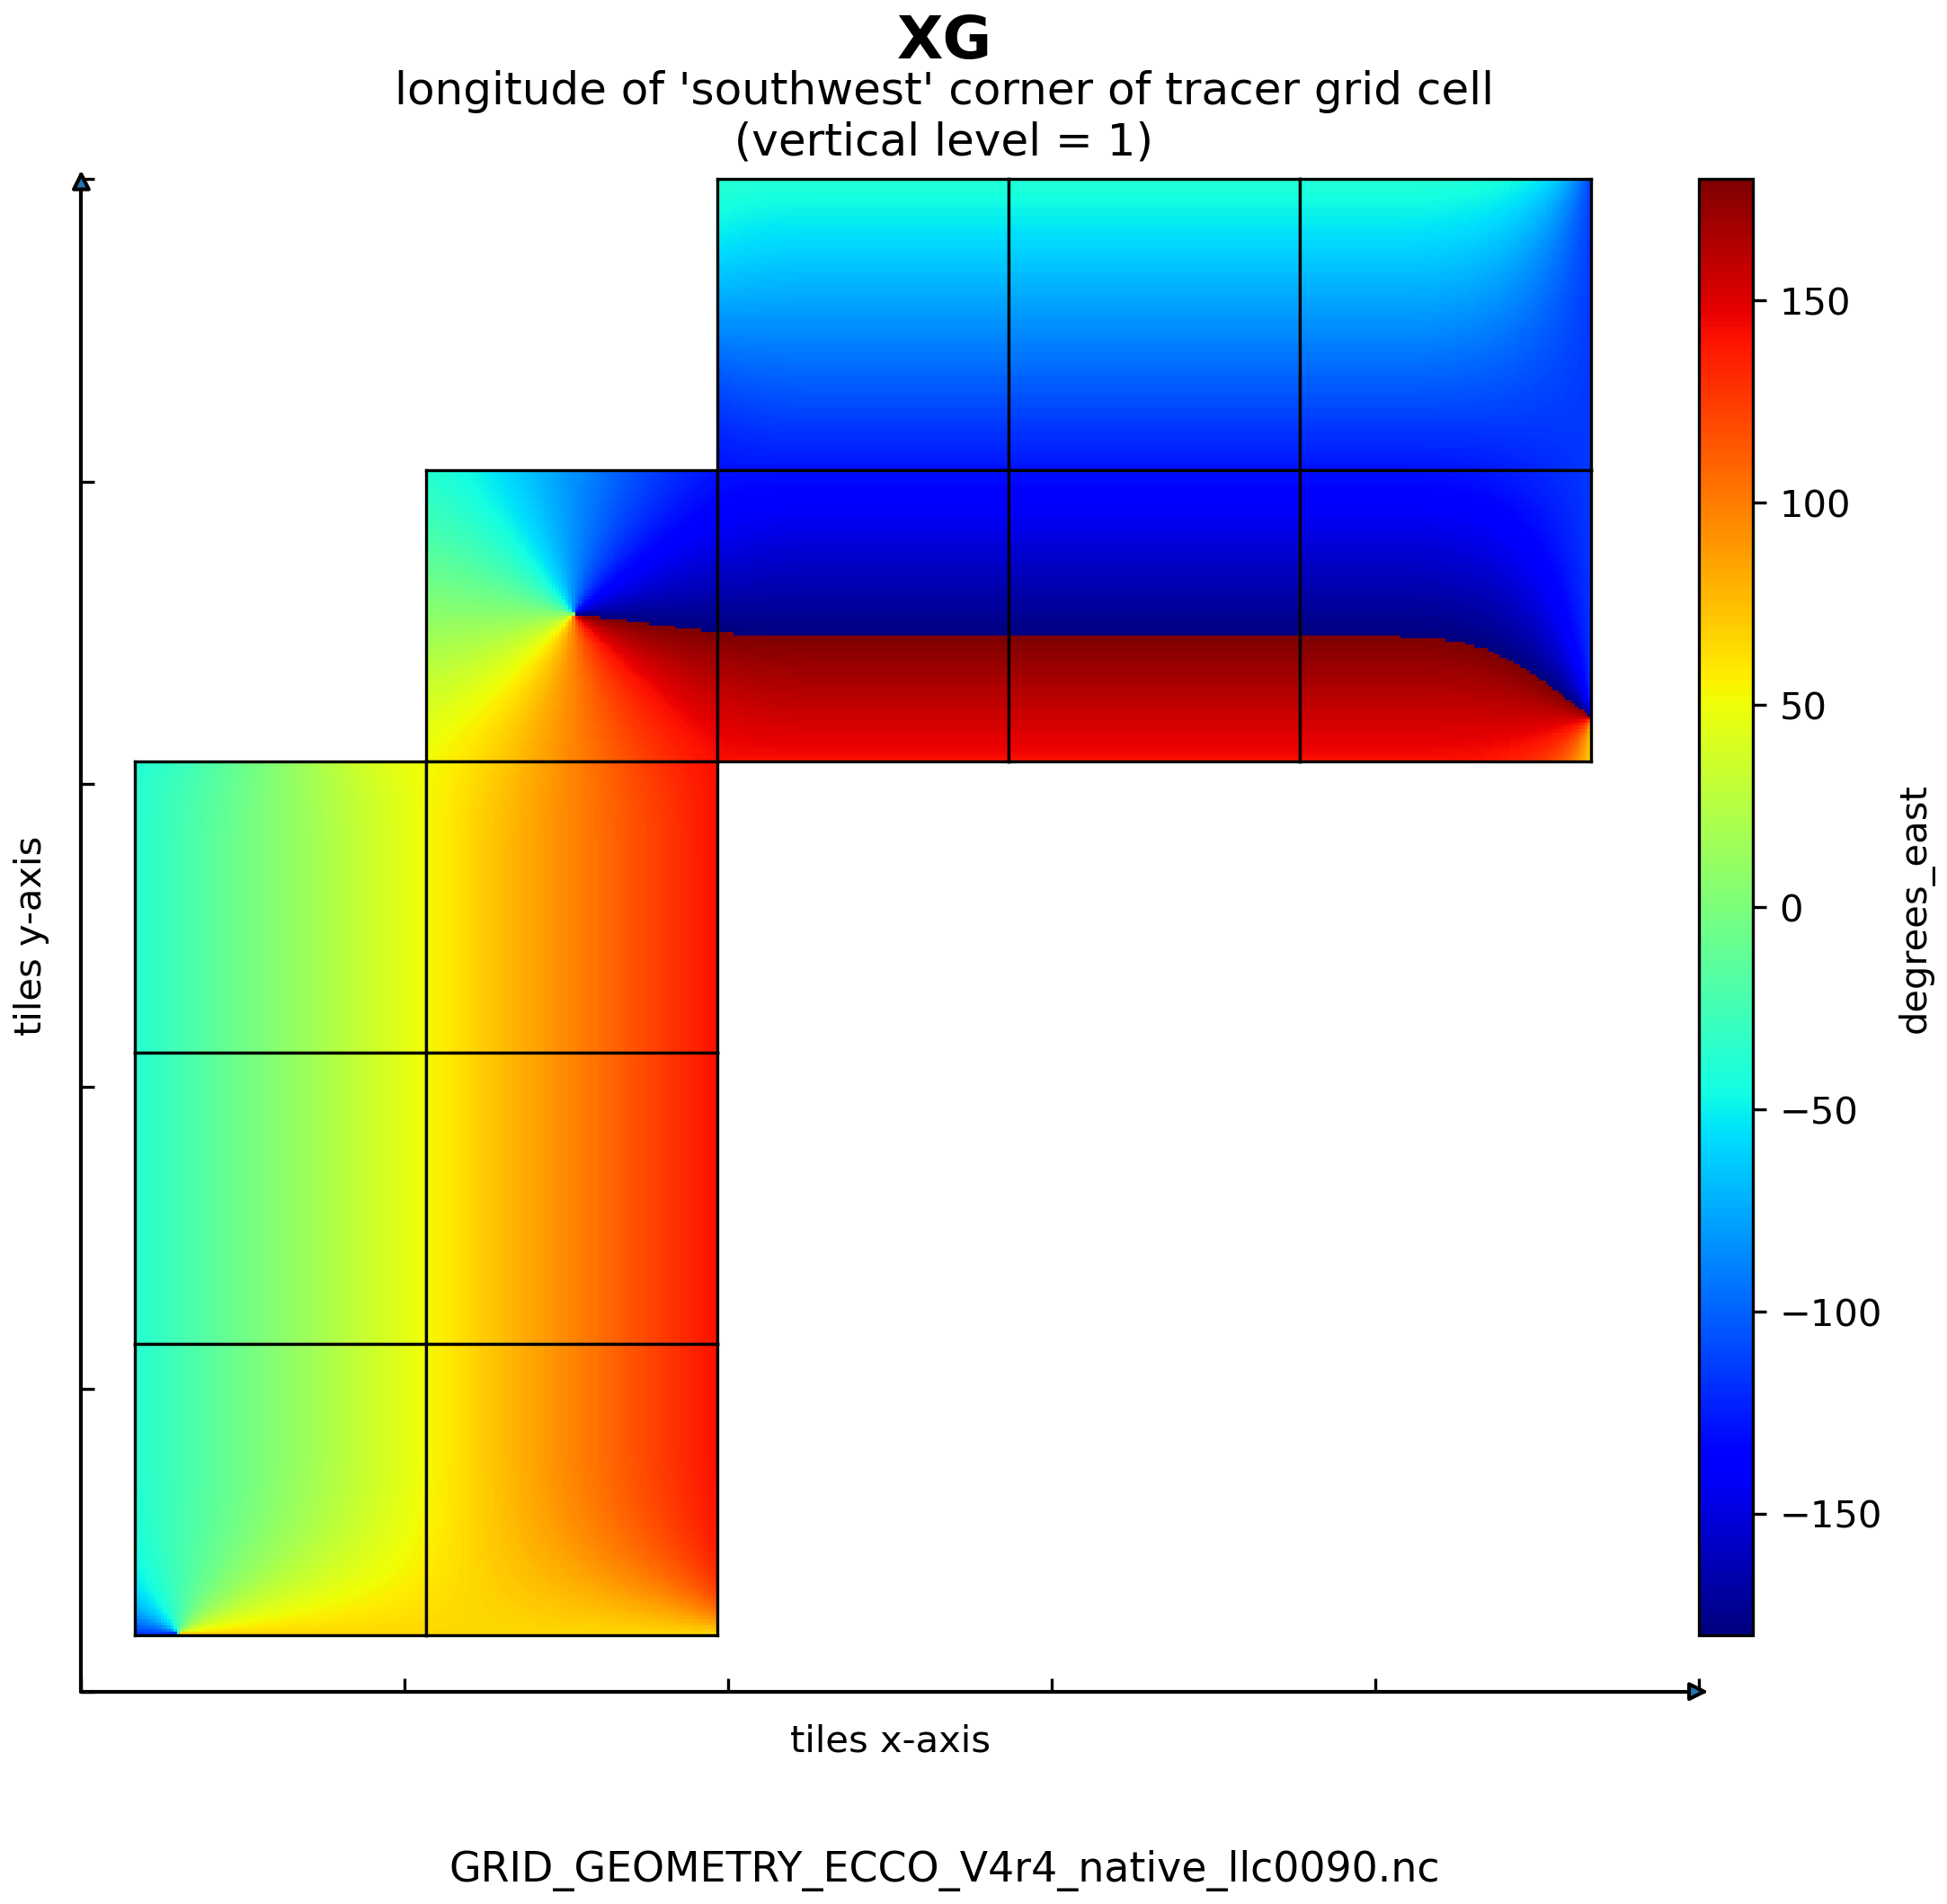
\includegraphics[scale=0.5]{../images/plots/native_plots_coords/Geometry_Parameters_for_the_Lat-Lon-Cap_90_(llc90)_Native_Model_Grid_(Version_4_Release_4)/XG.png}
\caption{\\Dataset: GRID\_GEOMETRY\_ECCO\\Variable: XG}
\label{tab:table-GRID_GEOMETRY_ECCO_XG-Plot}
\end{figure}
\pagebreak
\subsubsection{Native coordinates Variable YG}
\begin{longtable}{|p{0.06\textwidth}|p{0.41\textwidth}|p{0.39\textwidth}|p{0.06\textwidth}|}
    \caption{CDL description of GRID\_GEOMETRY\_ECCO's YG variable}
    \label{tab:table-GRID_GEOMETRY_ECCO_YG} \\ 
    \hline \endhead \hline \endfoot
    \rowcolor{lightgray} \textbf{Storage Type} & \textbf{Variable Name} & \textbf{Description} & \textbf{Unit} \\ \hline
    float32 & YG & latitude of 'southwest' corner of tracer grid cell & degrees\_north \\ \hline
    \rowcolor{lightgray}  \multicolumn{4}{|p{1.00\textwidth}|}{\textbf{CDL Description}} \\ \hline
    \multicolumn{4}{|p{1.00\textwidth}|}{\makecell{\parbox{1\textwidth}{float32 YG(tile, j\_g, i\_g)\\
    \hspace*{0.5cm}YG: long\_name = "latitude of southwest corner of tracer grid cell"\\
    \hspace*{0.5cm}YG: units = degrees\_north\\
    \hspace*{0.5cm}YG: coordinates =\hspace*{0.5cm} YG XG\\
    \hspace*{0.5cm}YG: coverage\_content\_type = coordinate\\
    \hspace*{0.5cm}YG: standard\_name = latitude}}} \\ \hline
    \rowcolor{lightgray} \multicolumn{4}{|p{1.00\textwidth}|}{\textbf{Comments}} \\ \hline
    \multicolumn{4}{|p{1\textwidth}|}{Nonuniform grid spacing. Note: 'southwest' does not correspond to geographic orientation but is used for convenience to describe the computational grid. See MITgcm dcoumentation for details.} \\ \hline
\end{longtable}

\begin{figure}[H]
\centering
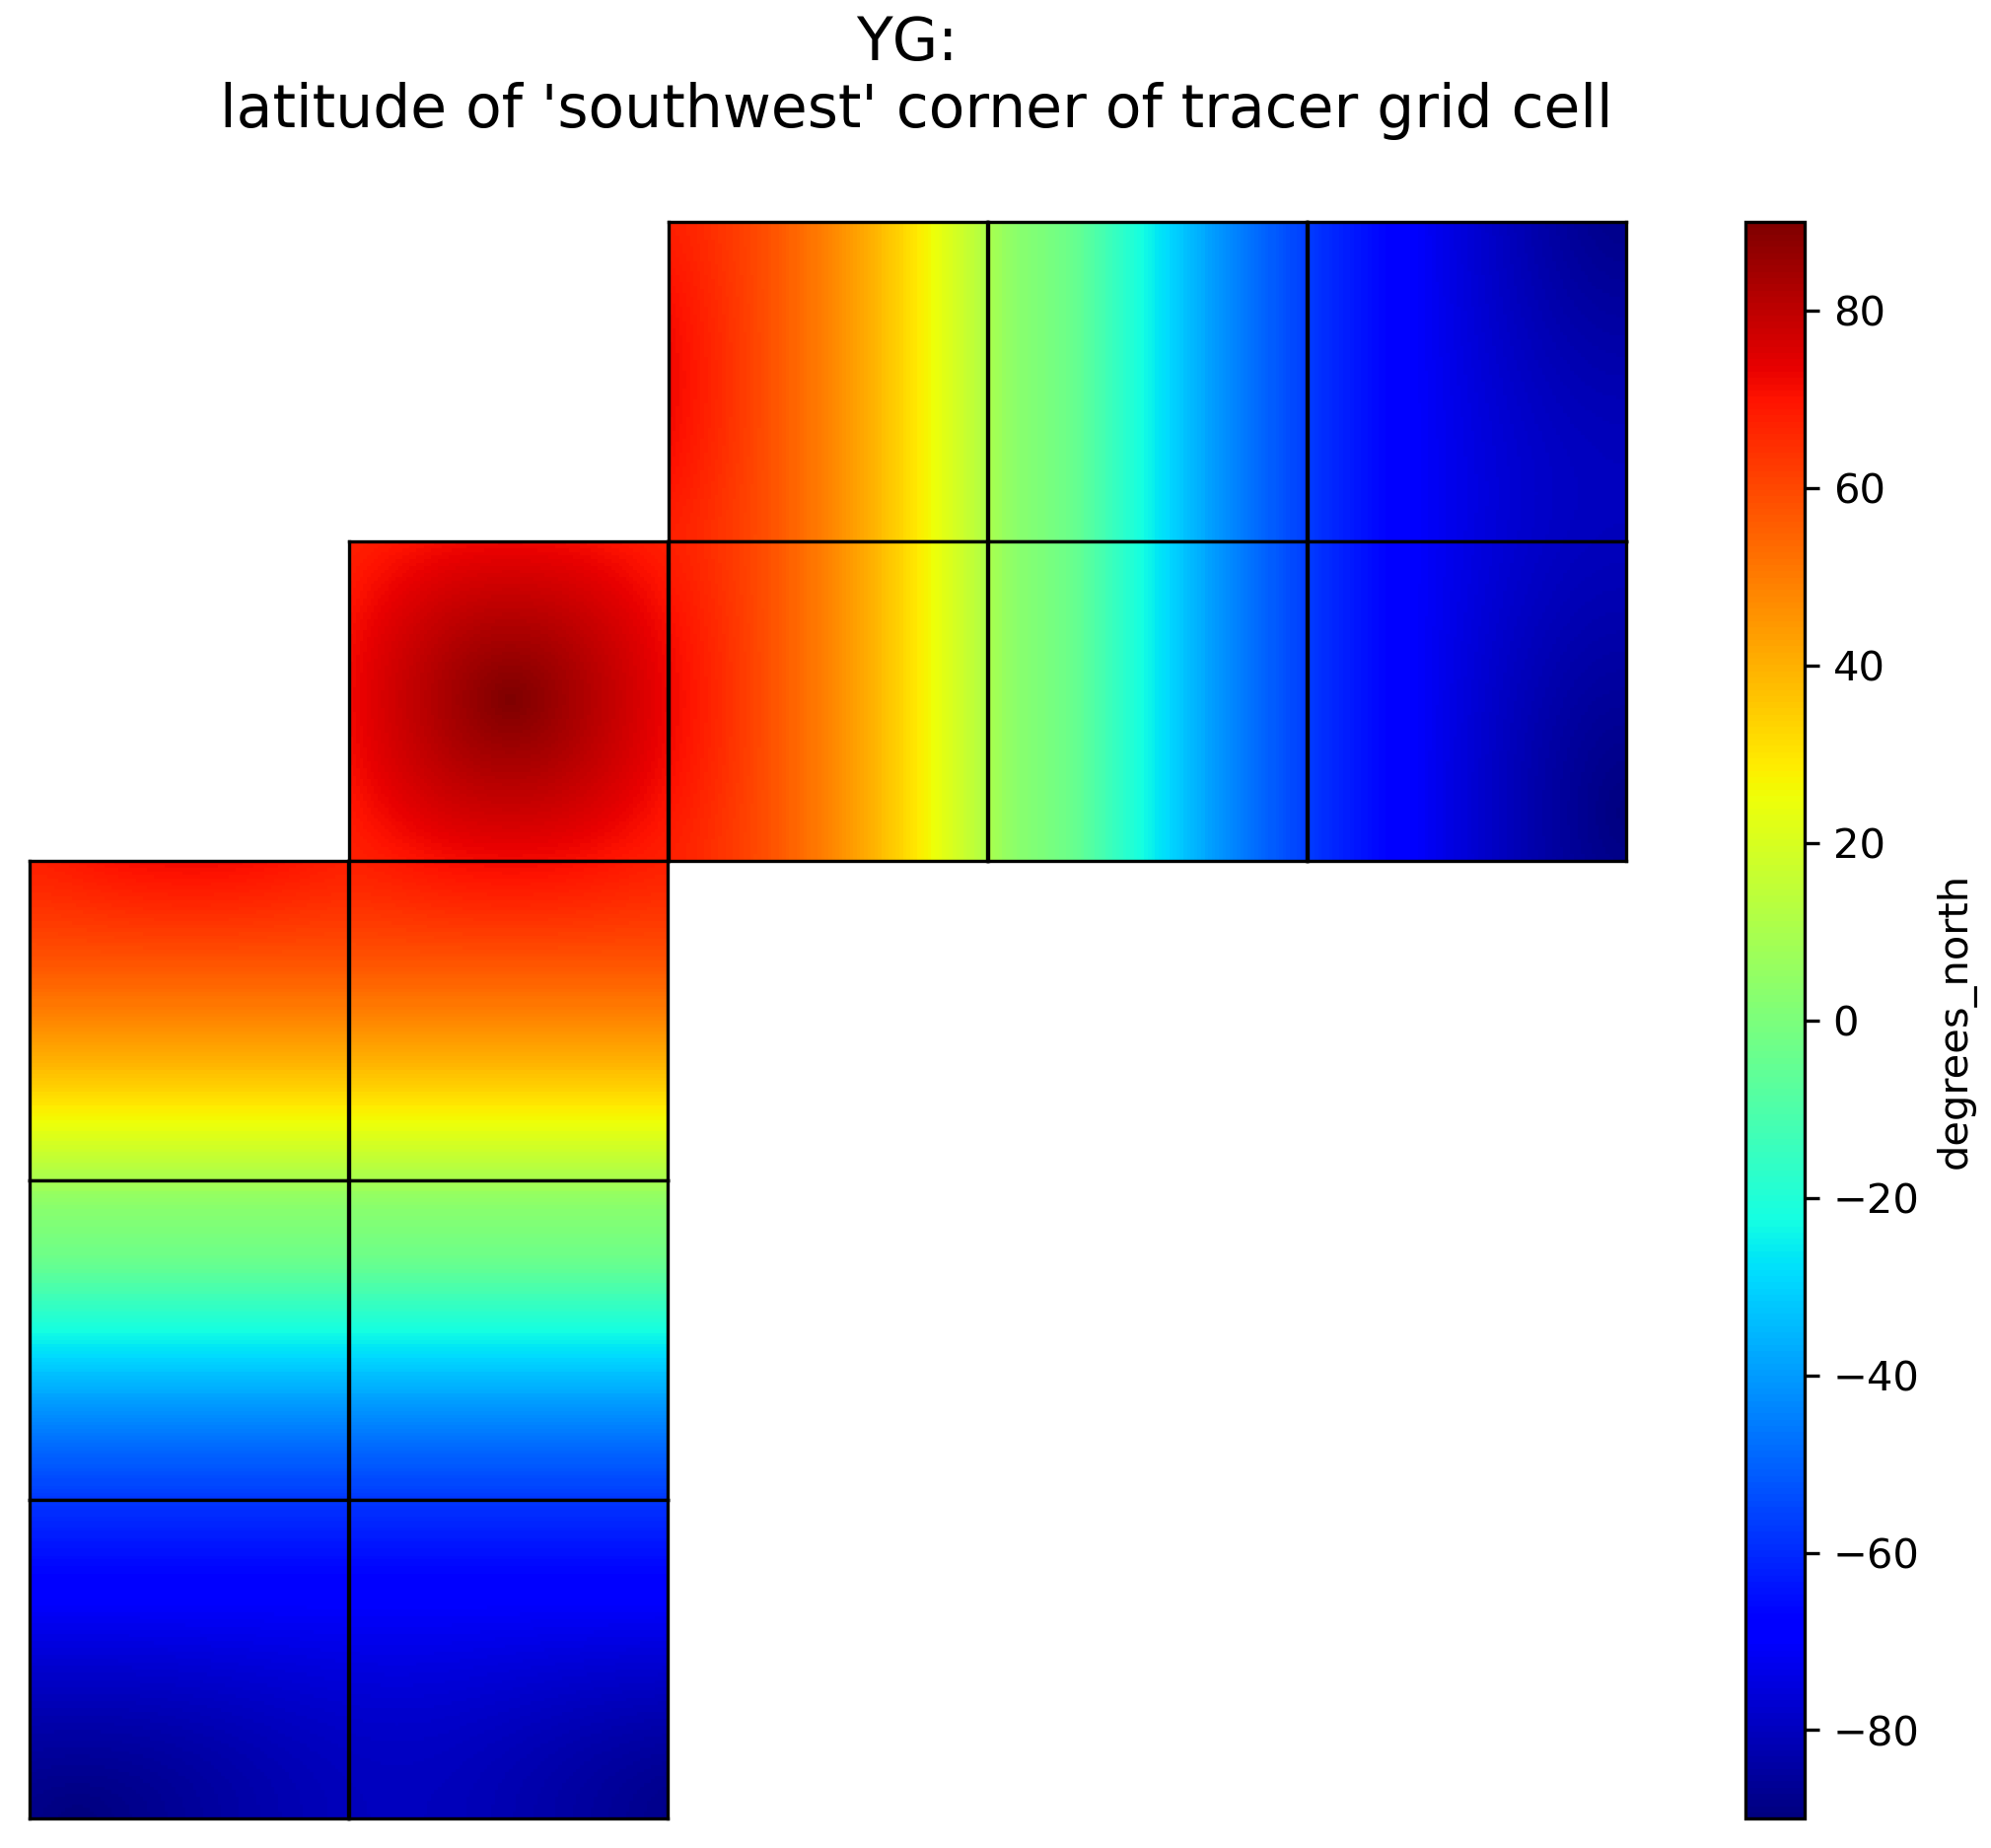
\includegraphics[scale=0.5]{../images/plots/native_plots_coords/Geometry_Parameters_for_the_Lat-Lon-Cap_90_(llc90)_Native_Model_Grid_(Version_4_Release_4)/YG.png}
\caption{\\Dataset: GRID\_GEOMETRY\_ECCO\\Variable: YG}
\label{tab:table-GRID_GEOMETRY_ECCO_YG-Plot}
\end{figure}
\pagebreak
\subsubsection{Native coordinates Variable CS}
\begin{longtable}{|p{0.06\textwidth}|p{0.41\textwidth}|p{0.39\textwidth}|p{0.06\textwidth}|}
    \caption{CDL description of GRID\_GEOMETRY\_ECCO's CS variable}
    \label{tab:table-GRID_GEOMETRY_ECCO_CS} \\ 
    \hline \endhead \hline \endfoot
    \rowcolor{lightgray} \textbf{Storage Type} & \textbf{Variable Name} & \textbf{Description} & \textbf{Unit} \\ \hline
    float32 & CS & cosine of tracer grid cell orientation vs geographical north & 1 \\ \hline
    \rowcolor{lightgray}  \multicolumn{4}{|p{1.00\textwidth}|}{\textbf{CDL Description}} \\ \hline
    \multicolumn{4}{|p{1.00\textwidth}|}{\makecell{\parbox{1\textwidth}{float32 CS(tile, j, i)\\
    \hspace*{0.5cm}CS: \_FillValue = 9.96921e+36\\
    \hspace*{0.5cm}CS: long\_name = cosine of tracer grid cell orientation vs geographical north\\
    \hspace*{0.5cm}CS: units = 1\\
    \hspace*{0.5cm}CS: coordinate = YC XC\\
    \hspace*{0.5cm}CS: coverage\_content\_type = modelResult\\
    \hspace*{0.5cm}CS: coordinates = YC XC}}} \\ \hline
    \rowcolor{lightgray} \multicolumn{4}{|p{1.00\textwidth}|}{\textbf{Comments}} \\ \hline
    \multicolumn{4}{|p{1\textwidth}|}{CS and SN are required to calculate the geographic (meridional, zonal) components of vectors on the curvilinear model grid. Note: for vector R with components R\_x and R\_y: R\_\{east\} = CS R\_x - SN R\_y.  R\_\{north\} = SN R\_x + CS R\_y} \\ \hline
\end{longtable}

\begin{figure}[H]
\centering
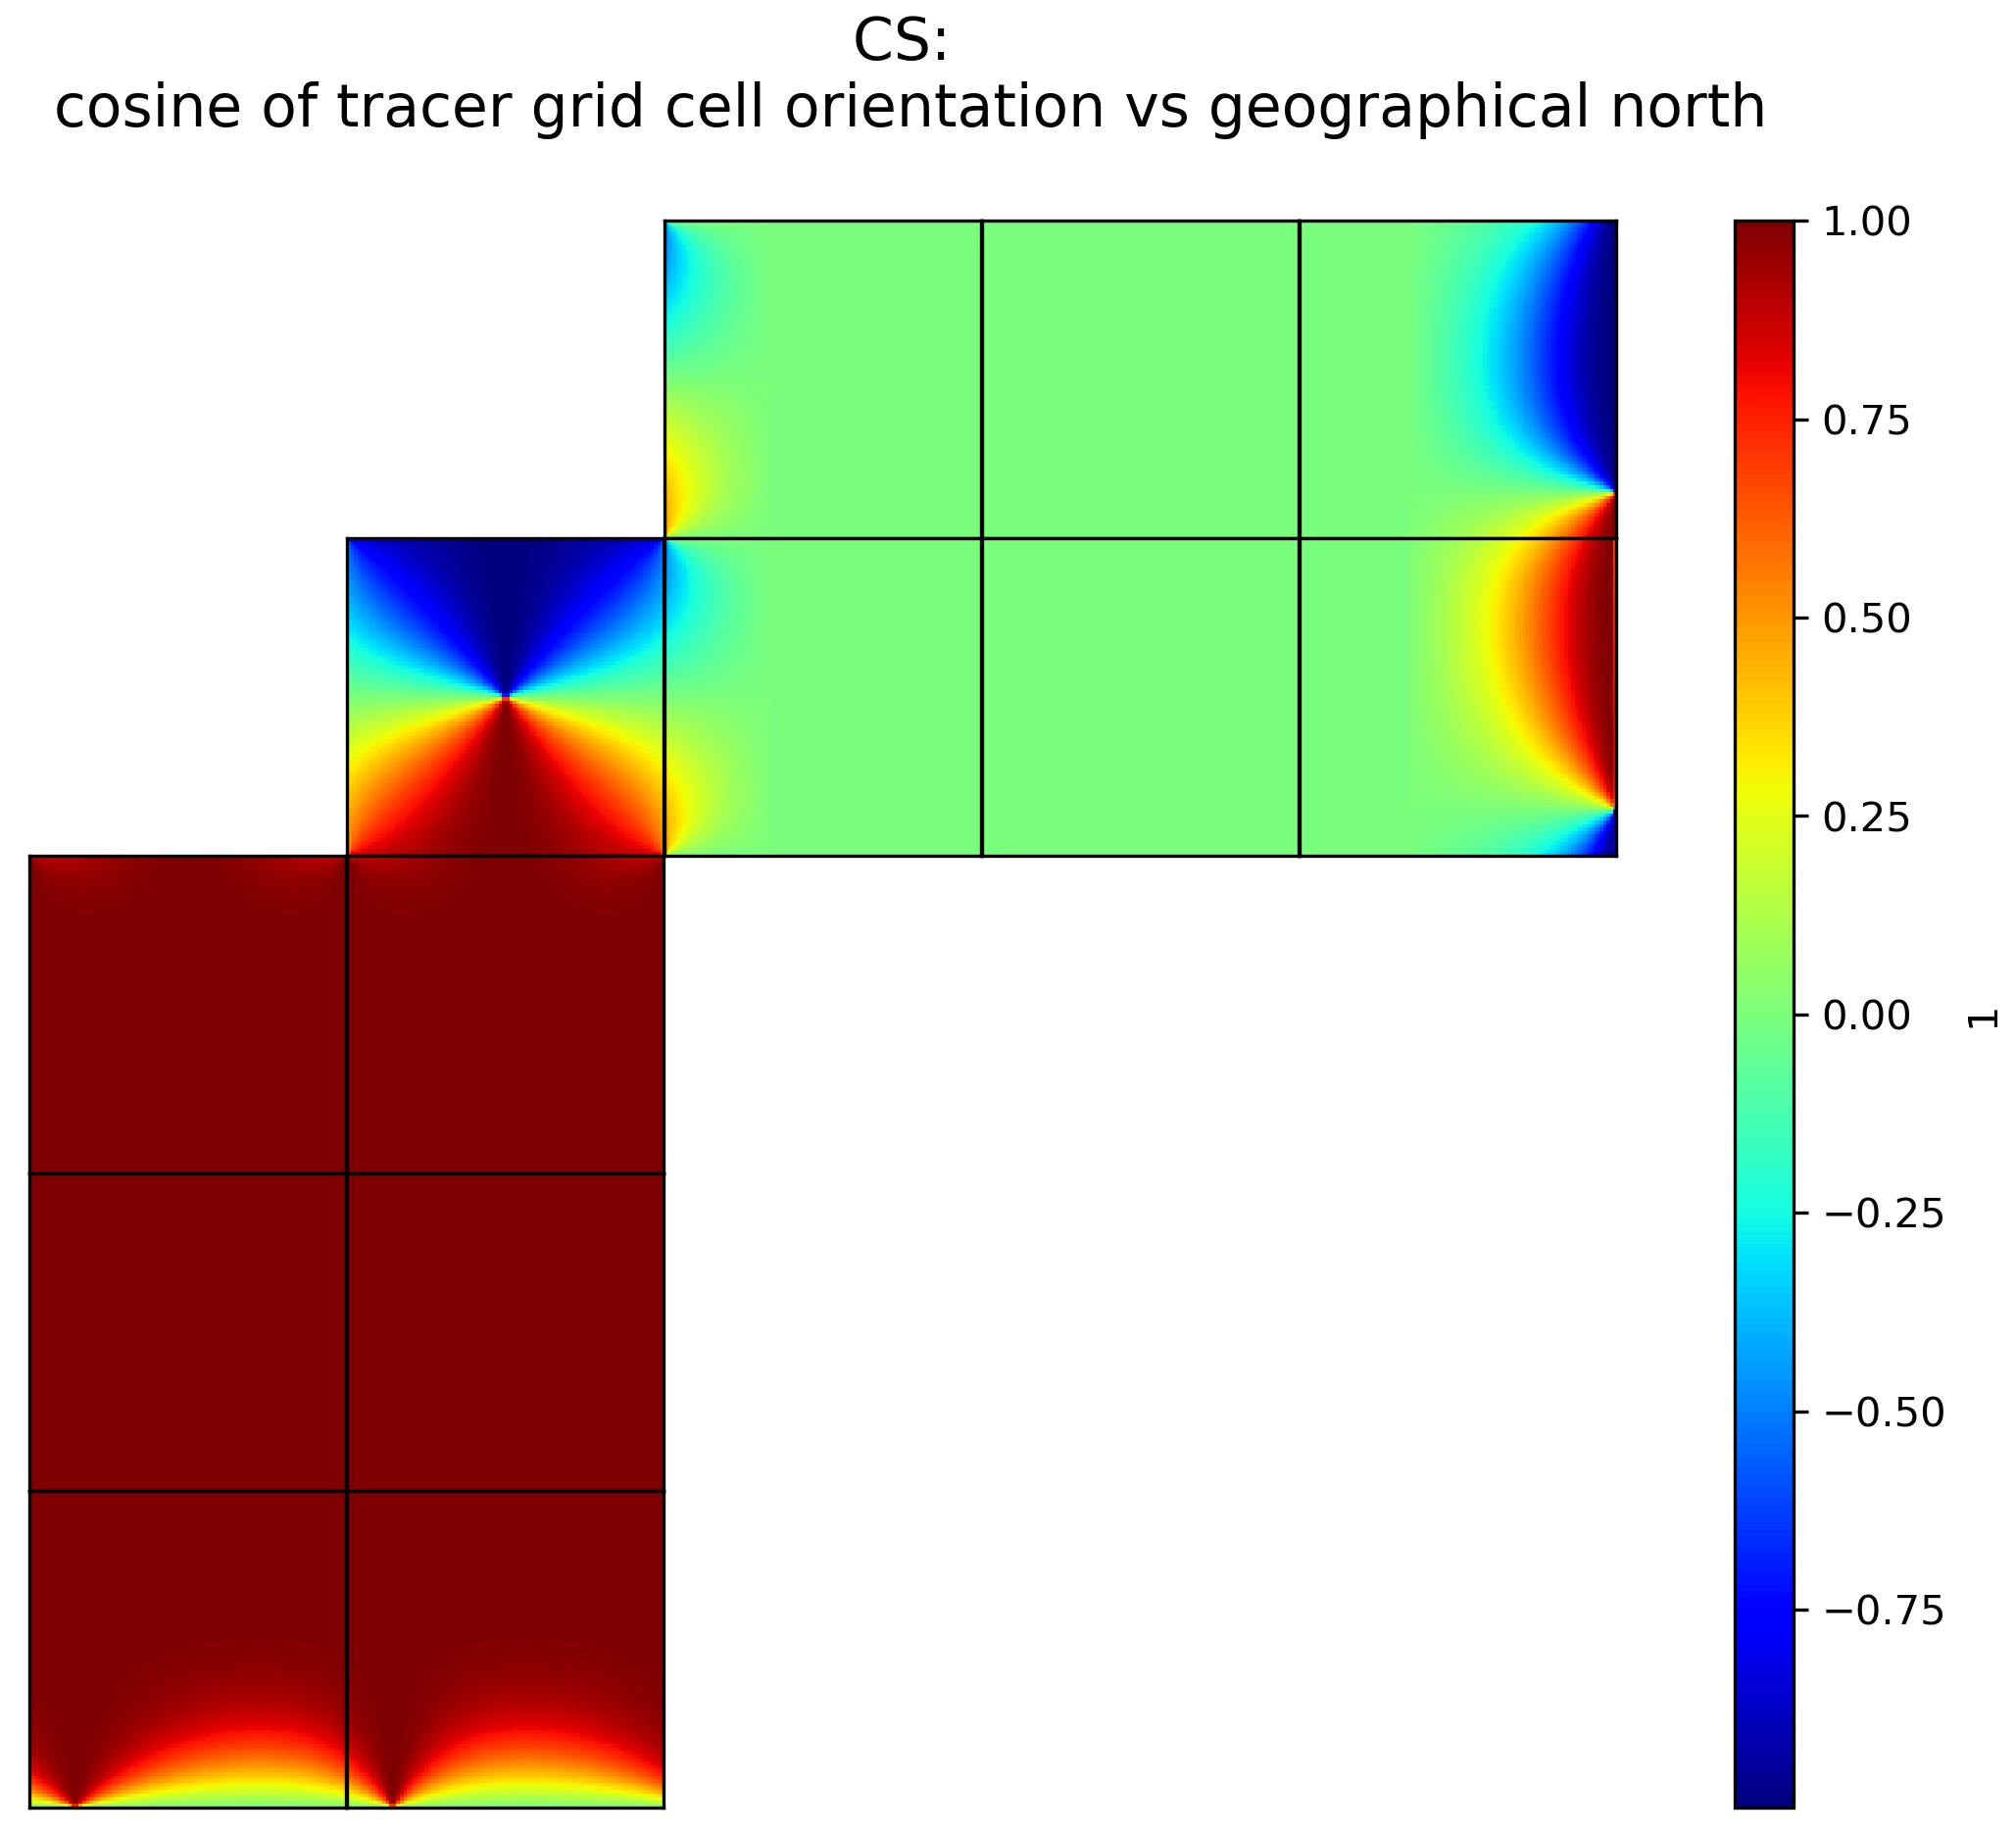
\includegraphics[scale=0.5]{../images/plots/native_plots_coords/Geometry_Parameters_for_the_Lat-Lon-Cap_90_(llc90)_Native_Model_Grid_(Version_4_Release_4)/CS.png}
\caption{\\Dataset: GRID\_GEOMETRY\_ECCO\\Variable: CS}
\label{tab:table-GRID_GEOMETRY_ECCO_CS-Plot}
\end{figure}
\pagebreak
\subsubsection{Native coordinates Variable SN}
\begin{longtable}{|p{0.06\textwidth}|p{0.41\textwidth}|p{0.39\textwidth}|p{0.06\textwidth}|}
    \caption{CDL description of GRID\_GEOMETRY\_ECCO's SN variable}
    \label{tab:table-GRID_GEOMETRY_ECCO_SN} \\ 
    \hline \endhead \hline \endfoot
    \rowcolor{lightgray} \textbf{Storage Type} & \textbf{Variable Name} & \textbf{Description} & \textbf{Unit} \\ \hline
    float32 & SN & sine of tracer grid cell orientation vs geographical north & 1 \\ \hline
    \rowcolor{lightgray}  \multicolumn{4}{|p{1.00\textwidth}|}{\textbf{CDL Description}} \\ \hline
    \multicolumn{4}{|p{1.00\textwidth}|}{\makecell{\parbox{1\textwidth}{float32 SN(tile, j, i)\\
    \hspace*{0.5cm}SN: \_FillValue = 9.96921e+36\\
    \hspace*{0.5cm}SN: long\_name = sine of tracer grid cell orientation vs geographical north\\
    \hspace*{0.5cm}SN: units = 1\\
    \hspace*{0.5cm}SN: coordinate = YC XC\\
    \hspace*{0.5cm}SN: coverage\_content\_type = modelResult\\
    \hspace*{0.5cm}SN: coordinates = YC XC}}} \\ \hline
    \rowcolor{lightgray} \multicolumn{4}{|p{1.00\textwidth}|}{\textbf{Comments}} \\ \hline
    \multicolumn{4}{|p{1\textwidth}|}{CS and SN are required to calculate the geographic (meridional, zonal) components of vectors on the curvilinear model grid. Note: for vector R with components R\_x and R\_y in local grid directions x and y, the geographical eastward component R\_\{east\} = CS R\_x - SN R\_y. The geographical northward component R\_\{north\} = SN R\_x + CS R\_y.} \\ \hline
\end{longtable}

\begin{figure}[H]
\centering
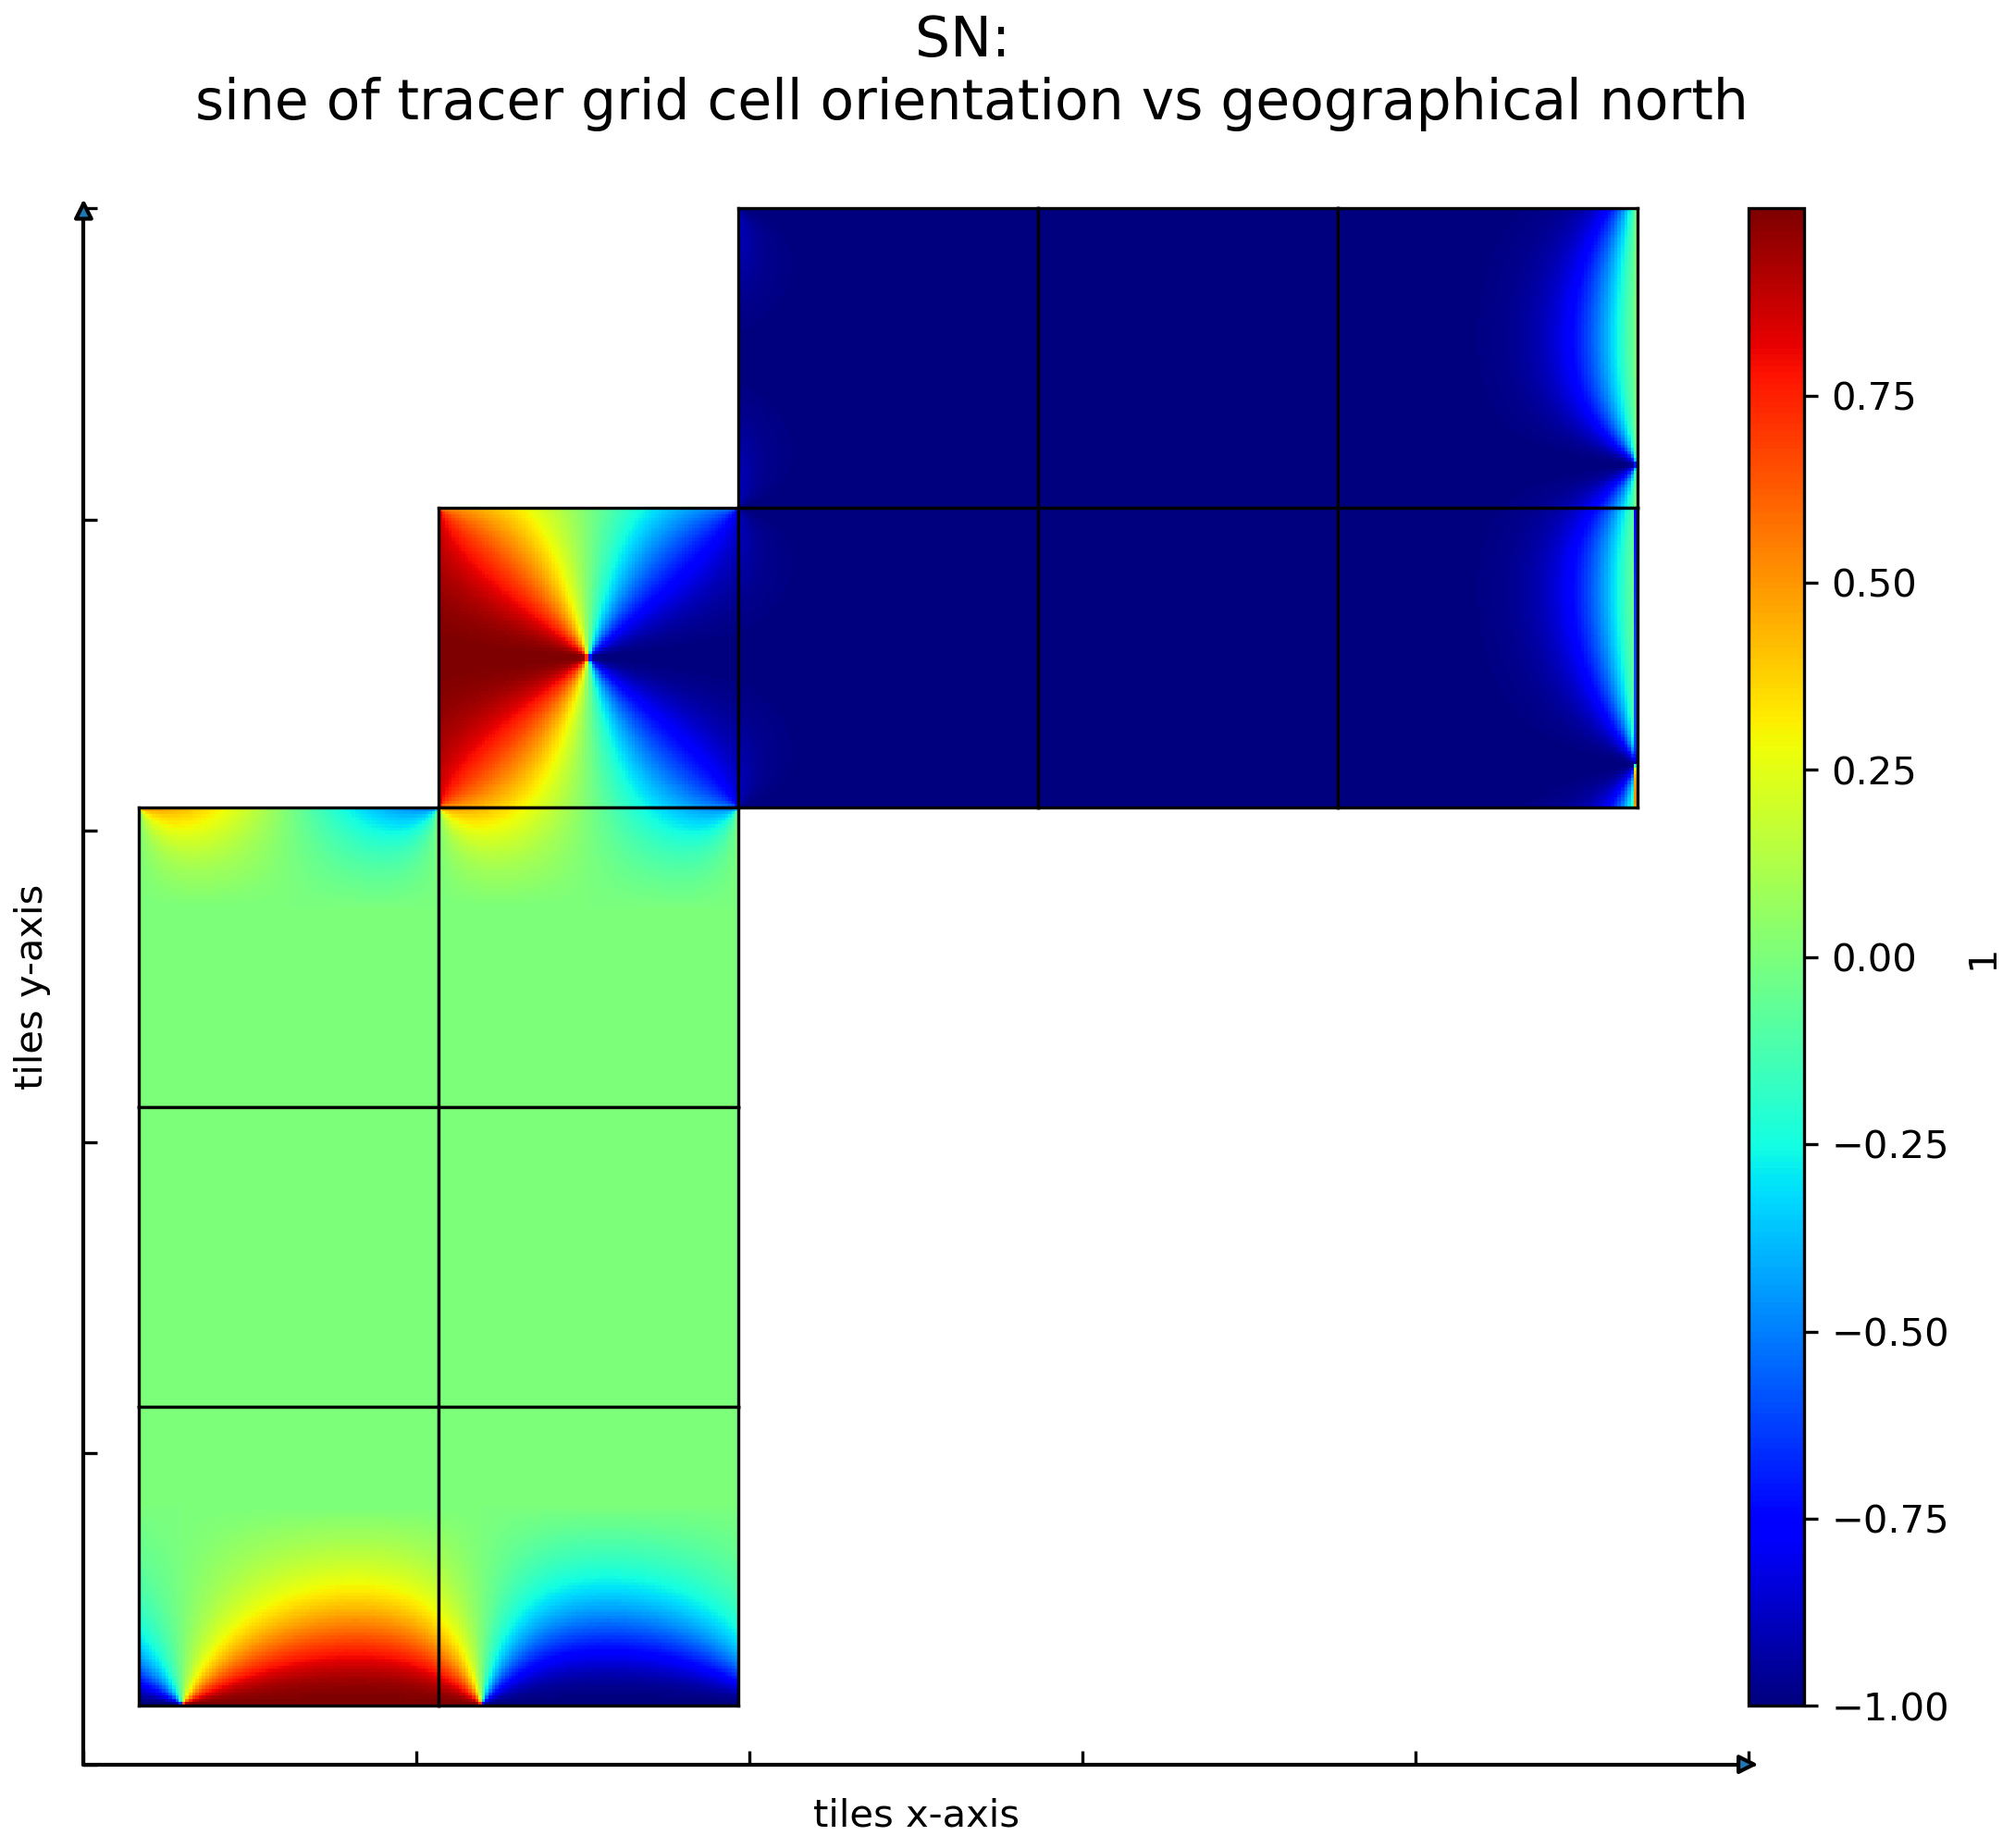
\includegraphics[scale=0.5]{../images/plots/native_plots_coords/Geometry_Parameters_for_the_Lat-Lon-Cap_90_(llc90)_Native_Model_Grid_(Version_4_Release_4)/SN.png}
\caption{\\Dataset: GRID\_GEOMETRY\_ECCO\\Variable: SN}
\label{tab:table-GRID_GEOMETRY_ECCO_SN-Plot}
\end{figure}
\pagebreak
\subsubsection{Native coordinates Variable rA}
    \begin{longtable}{|p{0.06\textwidth}|p{0.41\textwidth}|p{0.39\textwidth}|p{0.06\textwidth}|}
    \caption{CDL description of GRID\_GEOMETRY\_ECCO's rA variable}
    \label{tab:table-GRID_GEOMETRY_ECCO_rA} \\ 
    \hline \endhead \hline \endfoot
    \rowcolor{lightgray} \textbf{Storage Type} & \textbf{Variable Name} & \textbf{Description} & \textbf{Unit} \\ \hline
    float32 & rA & area of tracer grid cell & m2 \\ \hline
    \rowcolor{lightgray}  \multicolumn{4}{|p{1.00\textwidth}|}{\textbf{CDL Description}} \\ \hline
    \multicolumn{4}{|p{1.00\textwidth}|}{\makecell{\parbox{1\textwidth}{float32 rA(tile, j, i)\\
    \hspace*{0.5cm}rA: \_FillValue = 9.96921e+36\\
    \hspace*{0.5cm}rA: long\_name = area of tracer grid cell\\
    \hspace*{0.5cm}rA: units = m2\\
    \hspace*{0.5cm}rA: coordinate = YC XC\\
    \hspace*{0.5cm}rA: coverage\_content\_type = modelResult\\
    \hspace*{0.5cm}rA: standard\_name = cell\_area\\
    \hspace*{0.5cm}rA: coordinates = YC XC}}} \\ \hline
    \rowcolor{lightgray} \multicolumn{4}{|p{1.00\textwidth}|}{\textbf{Comments}} \\ \hline
    \multicolumn{4}{|p{1\textwidth}|}{N/A} \\ \hline
\end{longtable}

\begin{figure}[H]
\centering
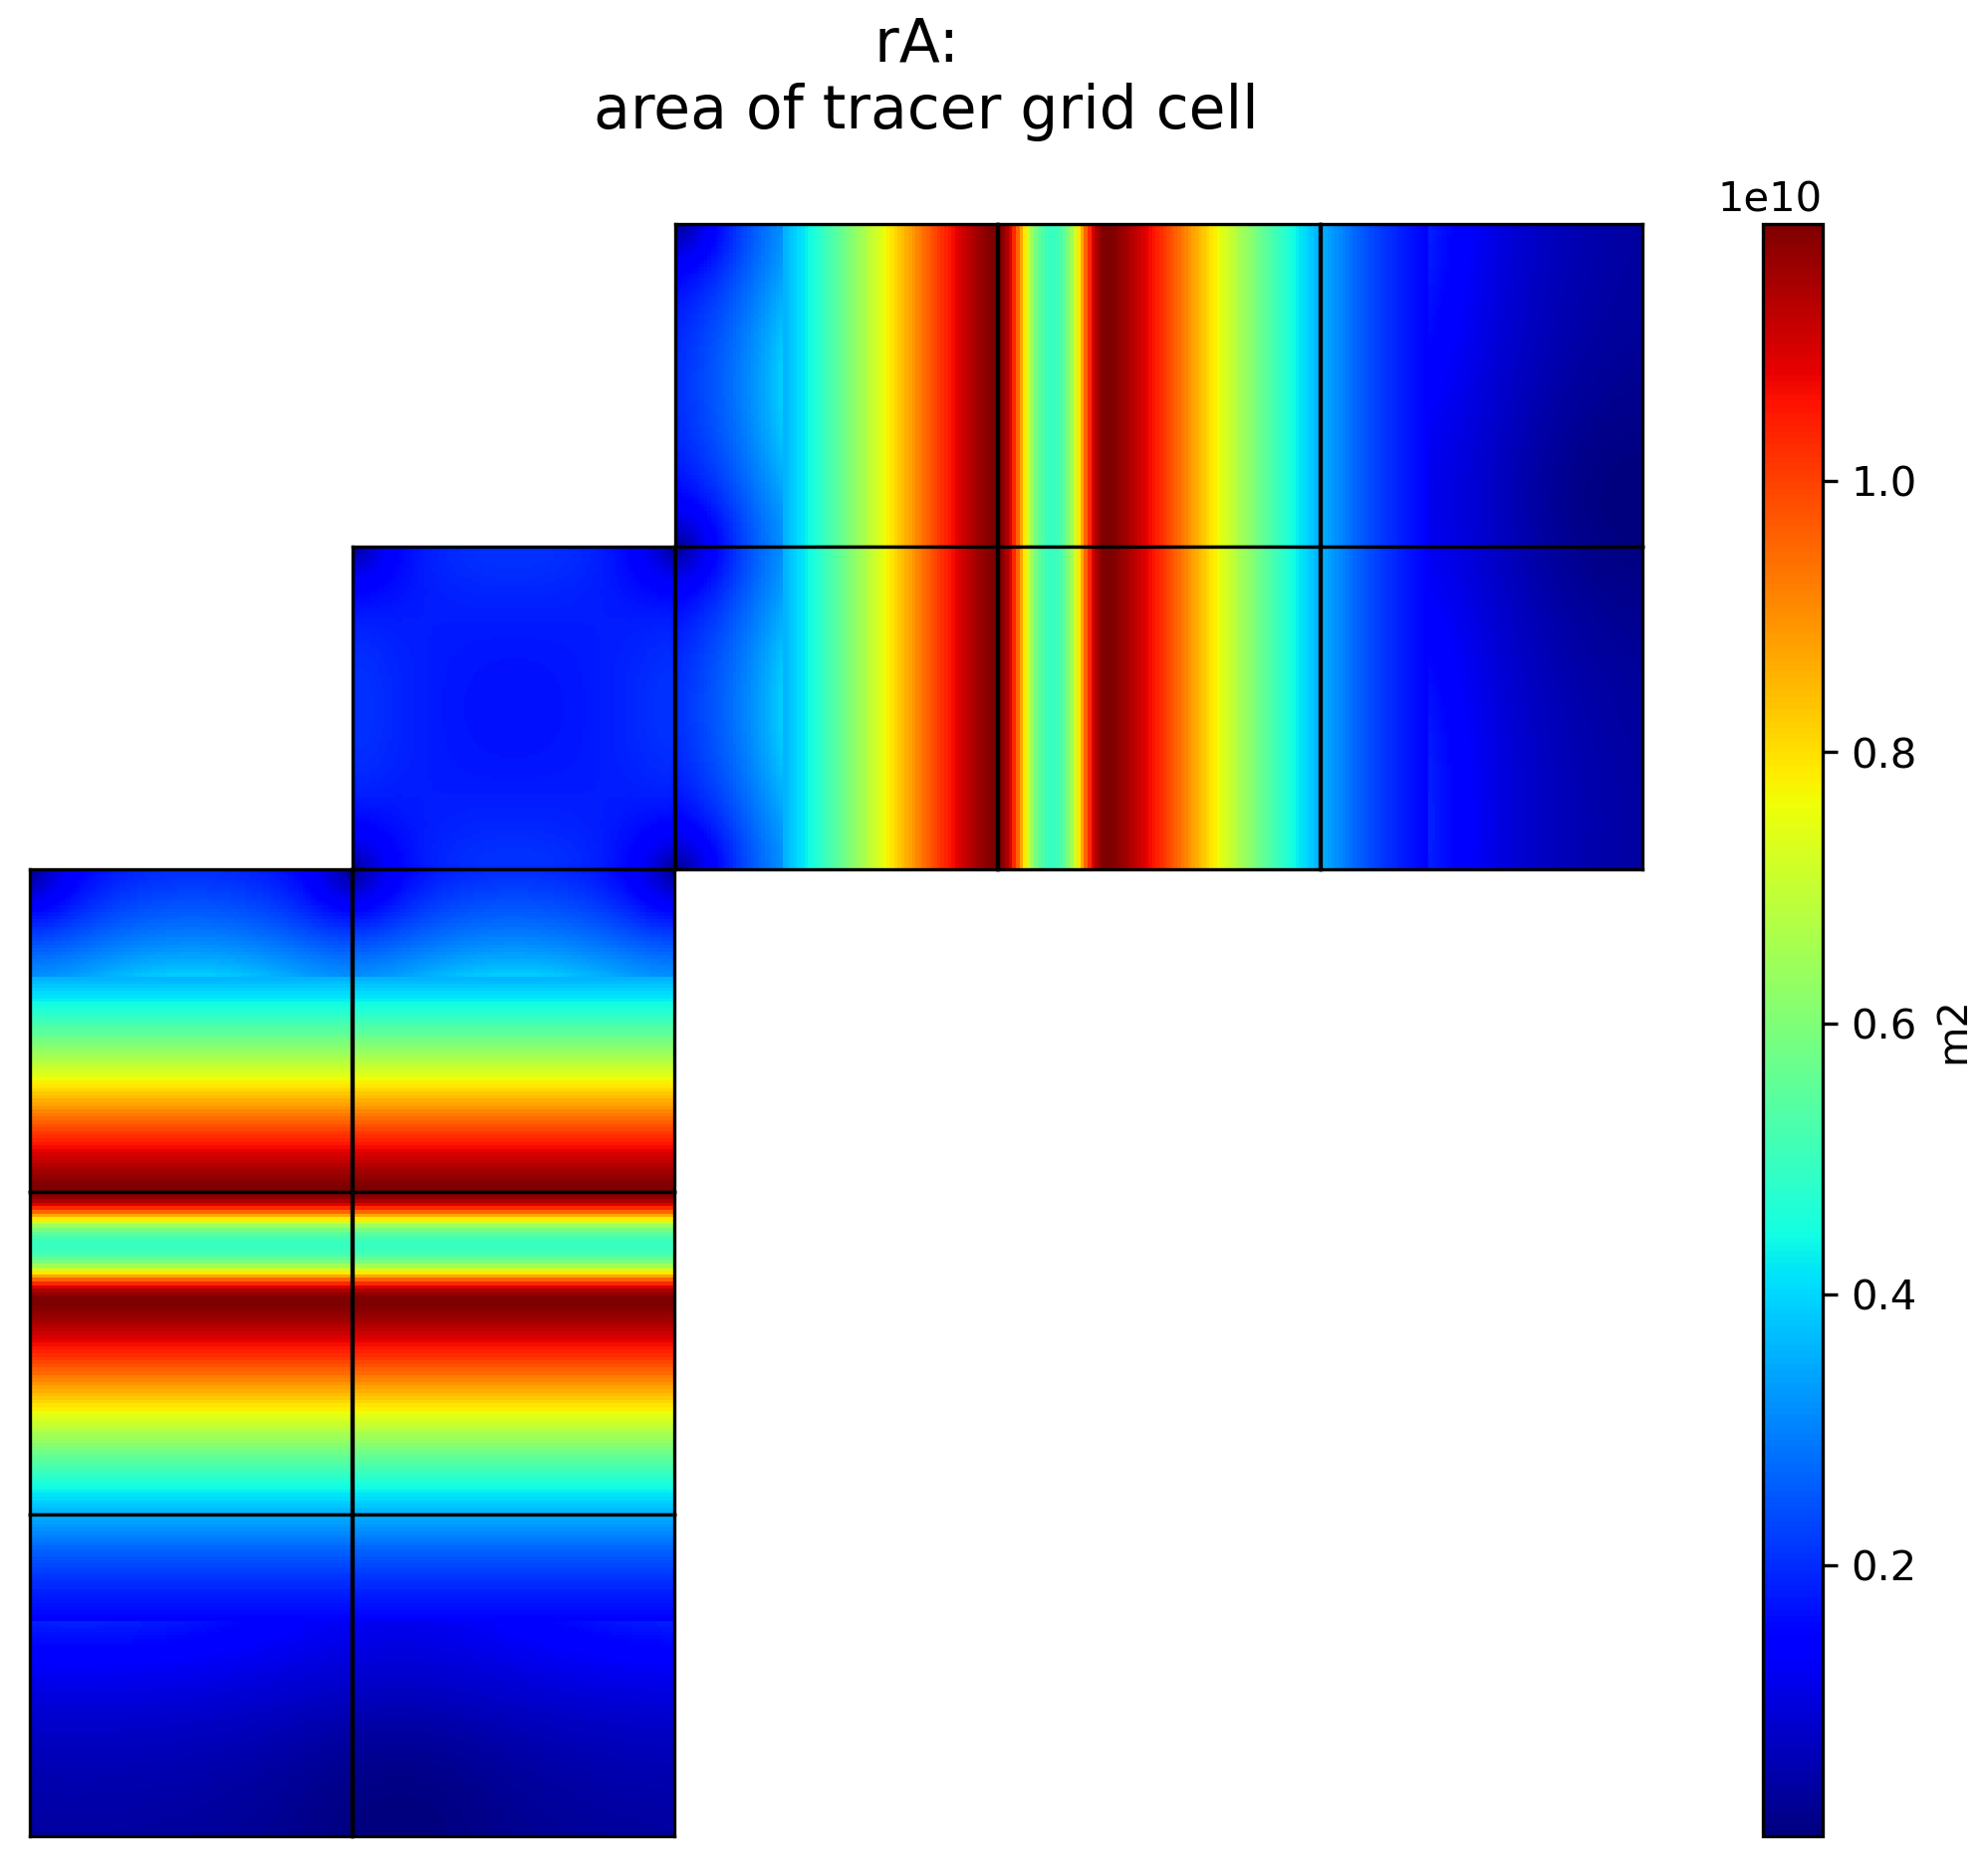
\includegraphics[scale=0.5]{../images/plots/native_plots_coords/Geometry_Parameters_for_the_Lat-Lon-Cap_90_(llc90)_Native_Model_Grid_(Version_4_Release_4)/rA.png}
\caption{\\Dataset: GRID\_GEOMETRY\_ECCO\\Variable: rA}
\label{tab:table-GRID_GEOMETRY_ECCO_rA-Plot}
\end{figure}
\pagebreak
\subsubsection{Native coordinates Variable dxG}
\begin{longtable}{|p{0.06\textwidth}|p{0.41\textwidth}|p{0.39\textwidth}|p{0.06\textwidth}|}
    \caption{CDL description of GRID\_GEOMETRY\_ECCO's dxG variable}
    \label{tab:table-GRID_GEOMETRY_ECCO_dxG} \\ 
    \hline \endhead \hline \endfoot
    \rowcolor{lightgray} \textbf{Storage Type} & \textbf{Variable Name} & \textbf{Description} & \textbf{Unit} \\ \hline
    float32 & dxG & distance between 'southwest' and 'southeast' corners of the tracer grid cell & m \\ \hline
    \rowcolor{lightgray}  \multicolumn{4}{|p{1.00\textwidth}|}{\textbf{CDL Description}} \\ \hline
    \multicolumn{4}{|p{1.00\textwidth}|}{\makecell{\parbox{1\textwidth}{float32 dxG(tile, j\_g, i)\\
    \hspace*{0.5cm}dxG: \_FillValue = 9.96921e+36\\
    \hspace*{0.5cm}dxG: long\_name = "distance between southwest and southeast corners of the tracer grid cell"\\
    \hspace*{0.5cm}dxG: units = m\\
    \hspace*{0.5cm}dxG: coordinate = YG XC\\
    \hspace*{0.5cm}dxG: coverage\_content\_type = modelResult}}} \\ \hline
    \rowcolor{lightgray} \multicolumn{4}{|p{1.00\textwidth}|}{\textbf{Comments}} \\ \hline
    \multicolumn{4}{|p{1\textwidth}|}{Alternatively, the length of 'south' side of tracer grid cell. Note: 'south', 'southwest', and 'southeast' do not correspond to geographic orientation but are used for convenience to describe the computational grid. See MITgcm documentation for details.} \\ \hline
\end{longtable}

\begin{figure}[H]
\centering
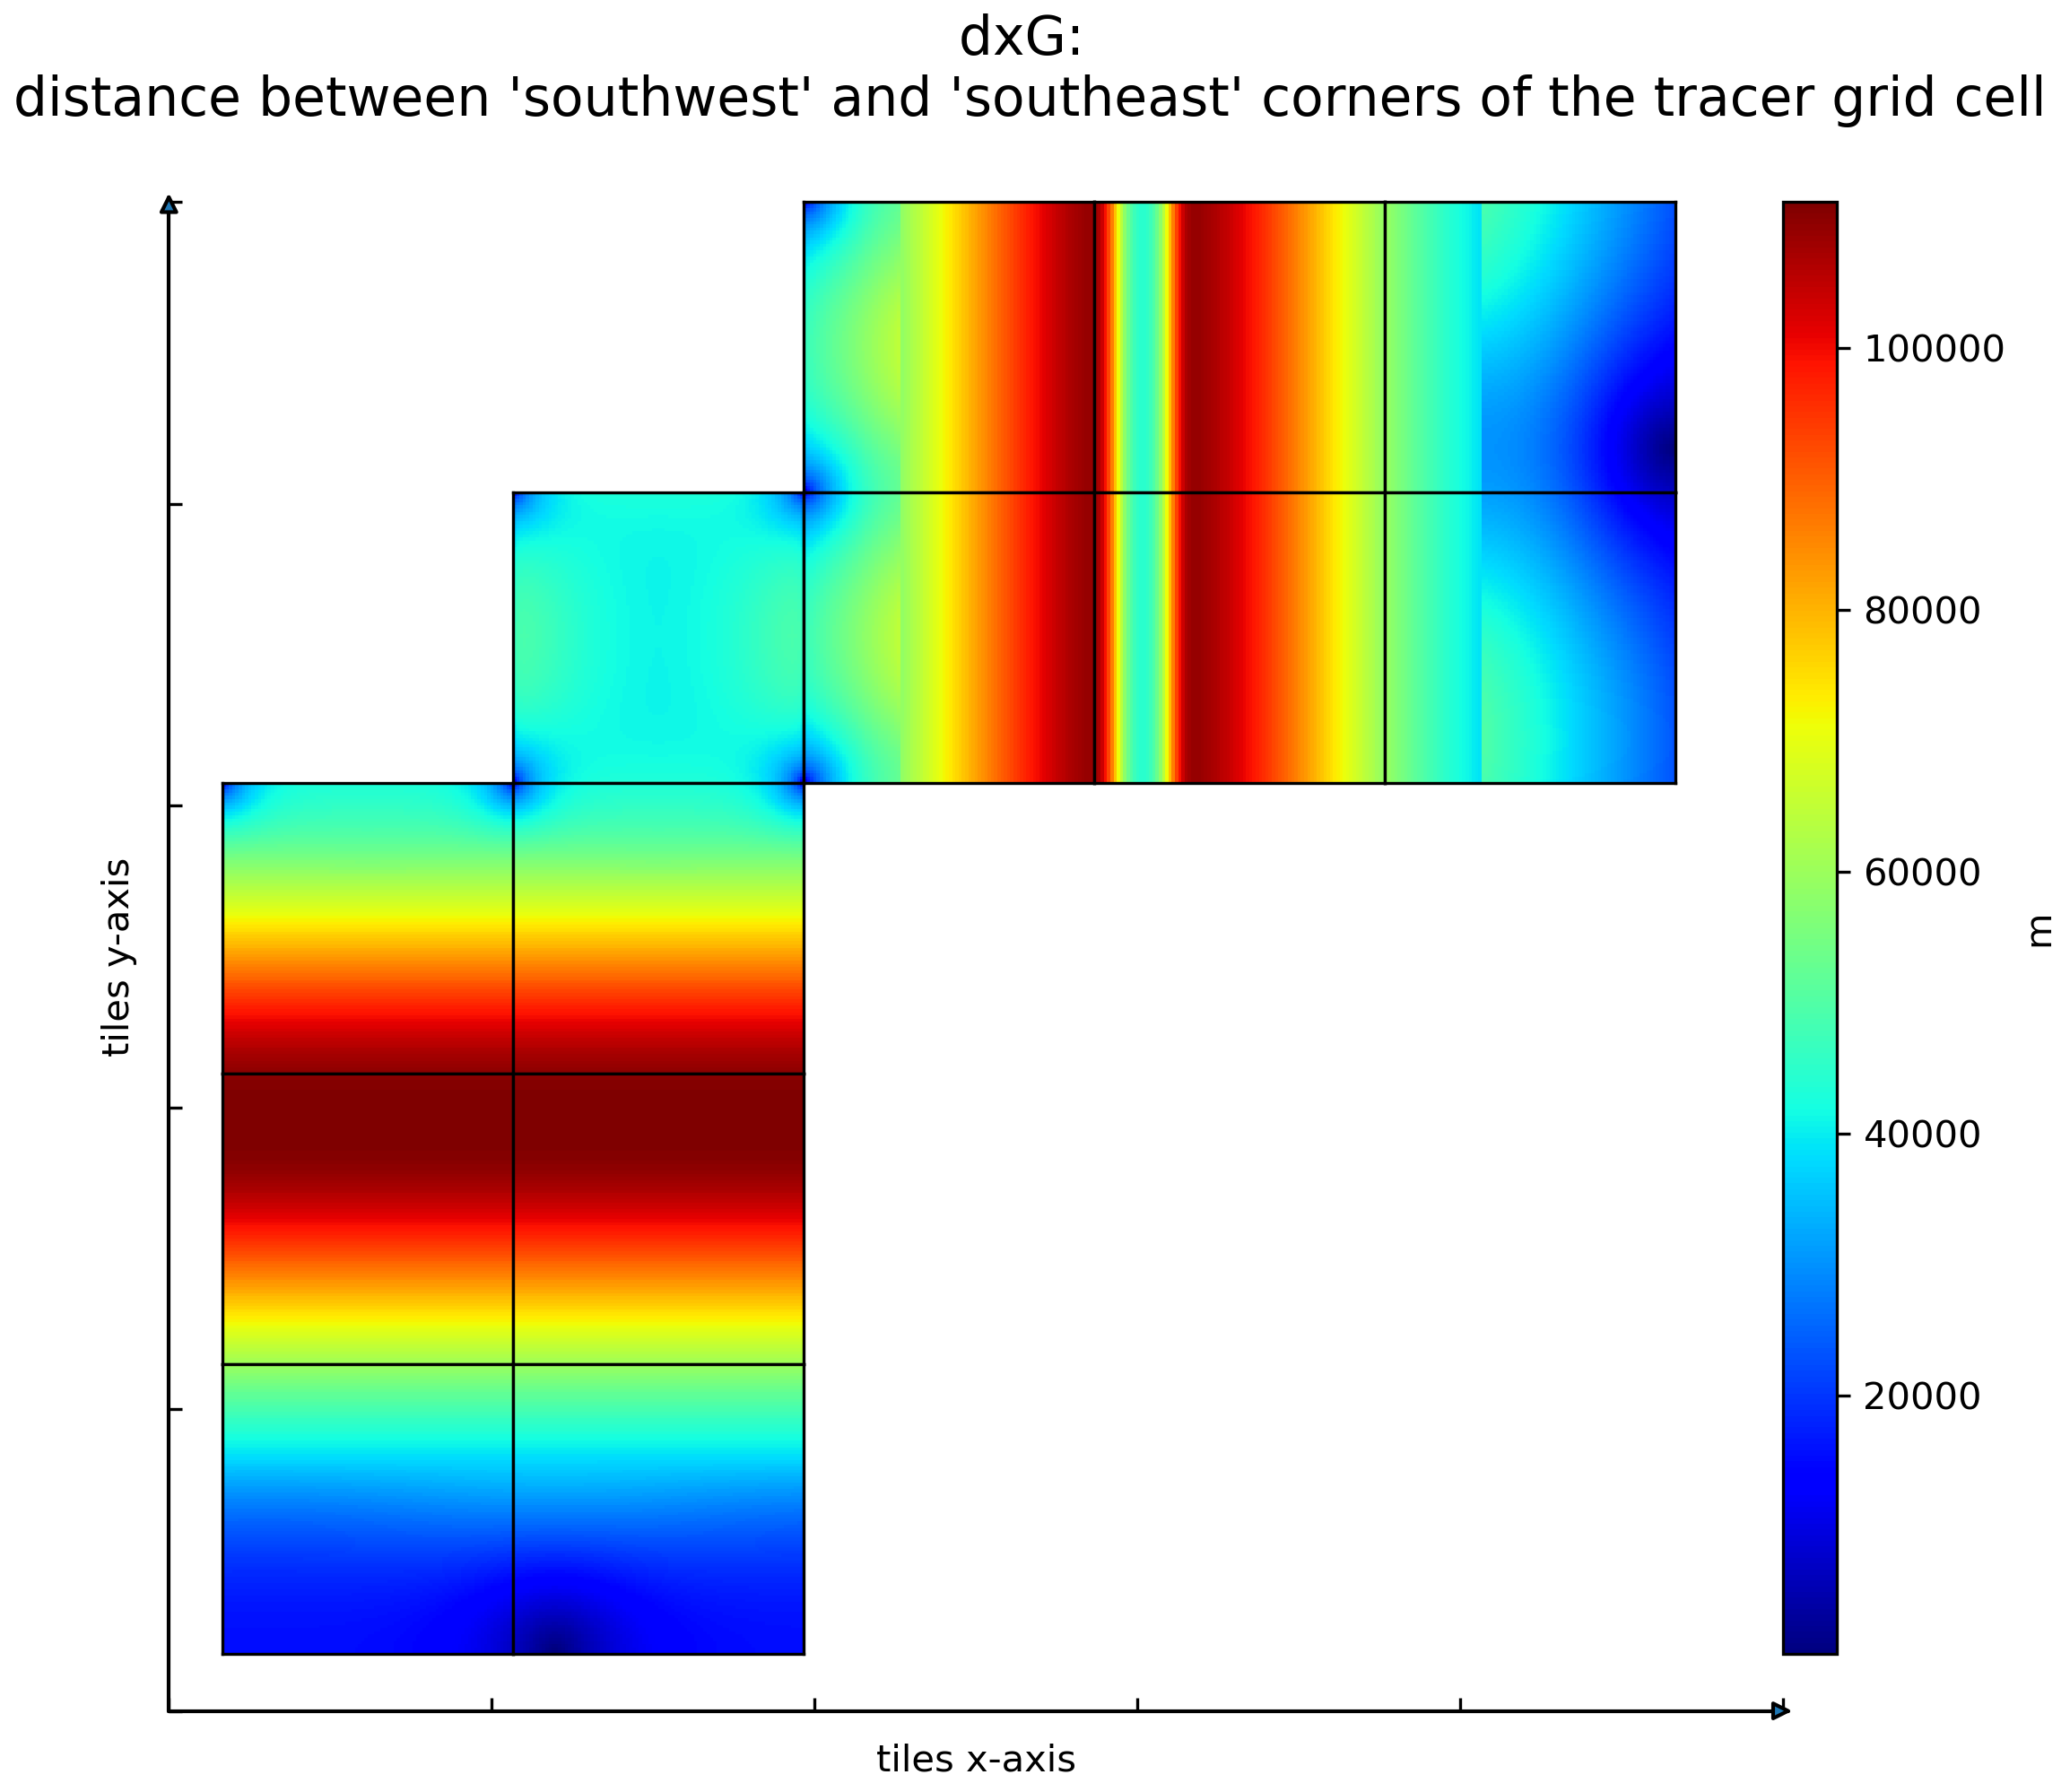
\includegraphics[scale=0.5]{../images/plots/native_plots_coords/Geometry_Parameters_for_the_Lat-Lon-Cap_90_(llc90)_Native_Model_Grid_(Version_4_Release_4)/dxG.png}
\caption{\\Dataset: GRID\_GEOMETRY\_ECCO\\Variable: dxG}
\label{tab:table-GRID_GEOMETRY_ECCO_dxG-Plot}
\end{figure}
\pagebreak
\subsubsection{Native coordinates Variable dyG}
\begin{longtable}{|p{0.06\textwidth}|p{0.41\textwidth}|p{0.39\textwidth}|p{0.06\textwidth}|}
    \caption{CDL description of GRID\_GEOMETRY\_ECCO's dyG variable}
    \label{tab:table-GRID_GEOMETRY_ECCO_dyG} \\ 
    \hline \endhead \hline \endfoot
    \rowcolor{lightgray} \textbf{Storage Type} & \textbf{Variable Name} & \textbf{Description} & \textbf{Unit} \\ \hline
    float32 & dyG & distance between 'southwest' and 'northwest' corners of the tracer grid cell & m \\ \hline
    \rowcolor{lightgray}  \multicolumn{4}{|p{1.00\textwidth}|}{\textbf{CDL Description}} \\ \hline
    \multicolumn{4}{|p{1.00\textwidth}|}{\makecell{\parbox{1\textwidth}{float32 dyG(tile, j, i\_g)\\
    \hspace*{0.5cm}dyG: \_FillValue = 9.96921e+36\\
    \hspace*{0.5cm}dyG: long\_name = "distance between southwest and northwest corners of the tracer grid cell"\\
    \hspace*{0.5cm}dyG: units = m\\
    \hspace*{0.5cm}dyG: coordinate = YC XG\\
    \hspace*{0.5cm}dyG: coverage\_content\_type = modelResult}}} \\ \hline
    \rowcolor{lightgray} \multicolumn{4}{|p{1.00\textwidth}|}{\textbf{Comments}} \\ \hline
    \multicolumn{4}{|p{1\textwidth}|}{Alternatively, the length of 'west' side of tracer grid cell. Note: 'west, 'southwest', and 'northwest' do not correspond to geographic orientation but are used for convenience to describe the computational grid. See MITgcm documentation for details.} \\ \hline
\end{longtable}

\begin{figure}[H]
\centering
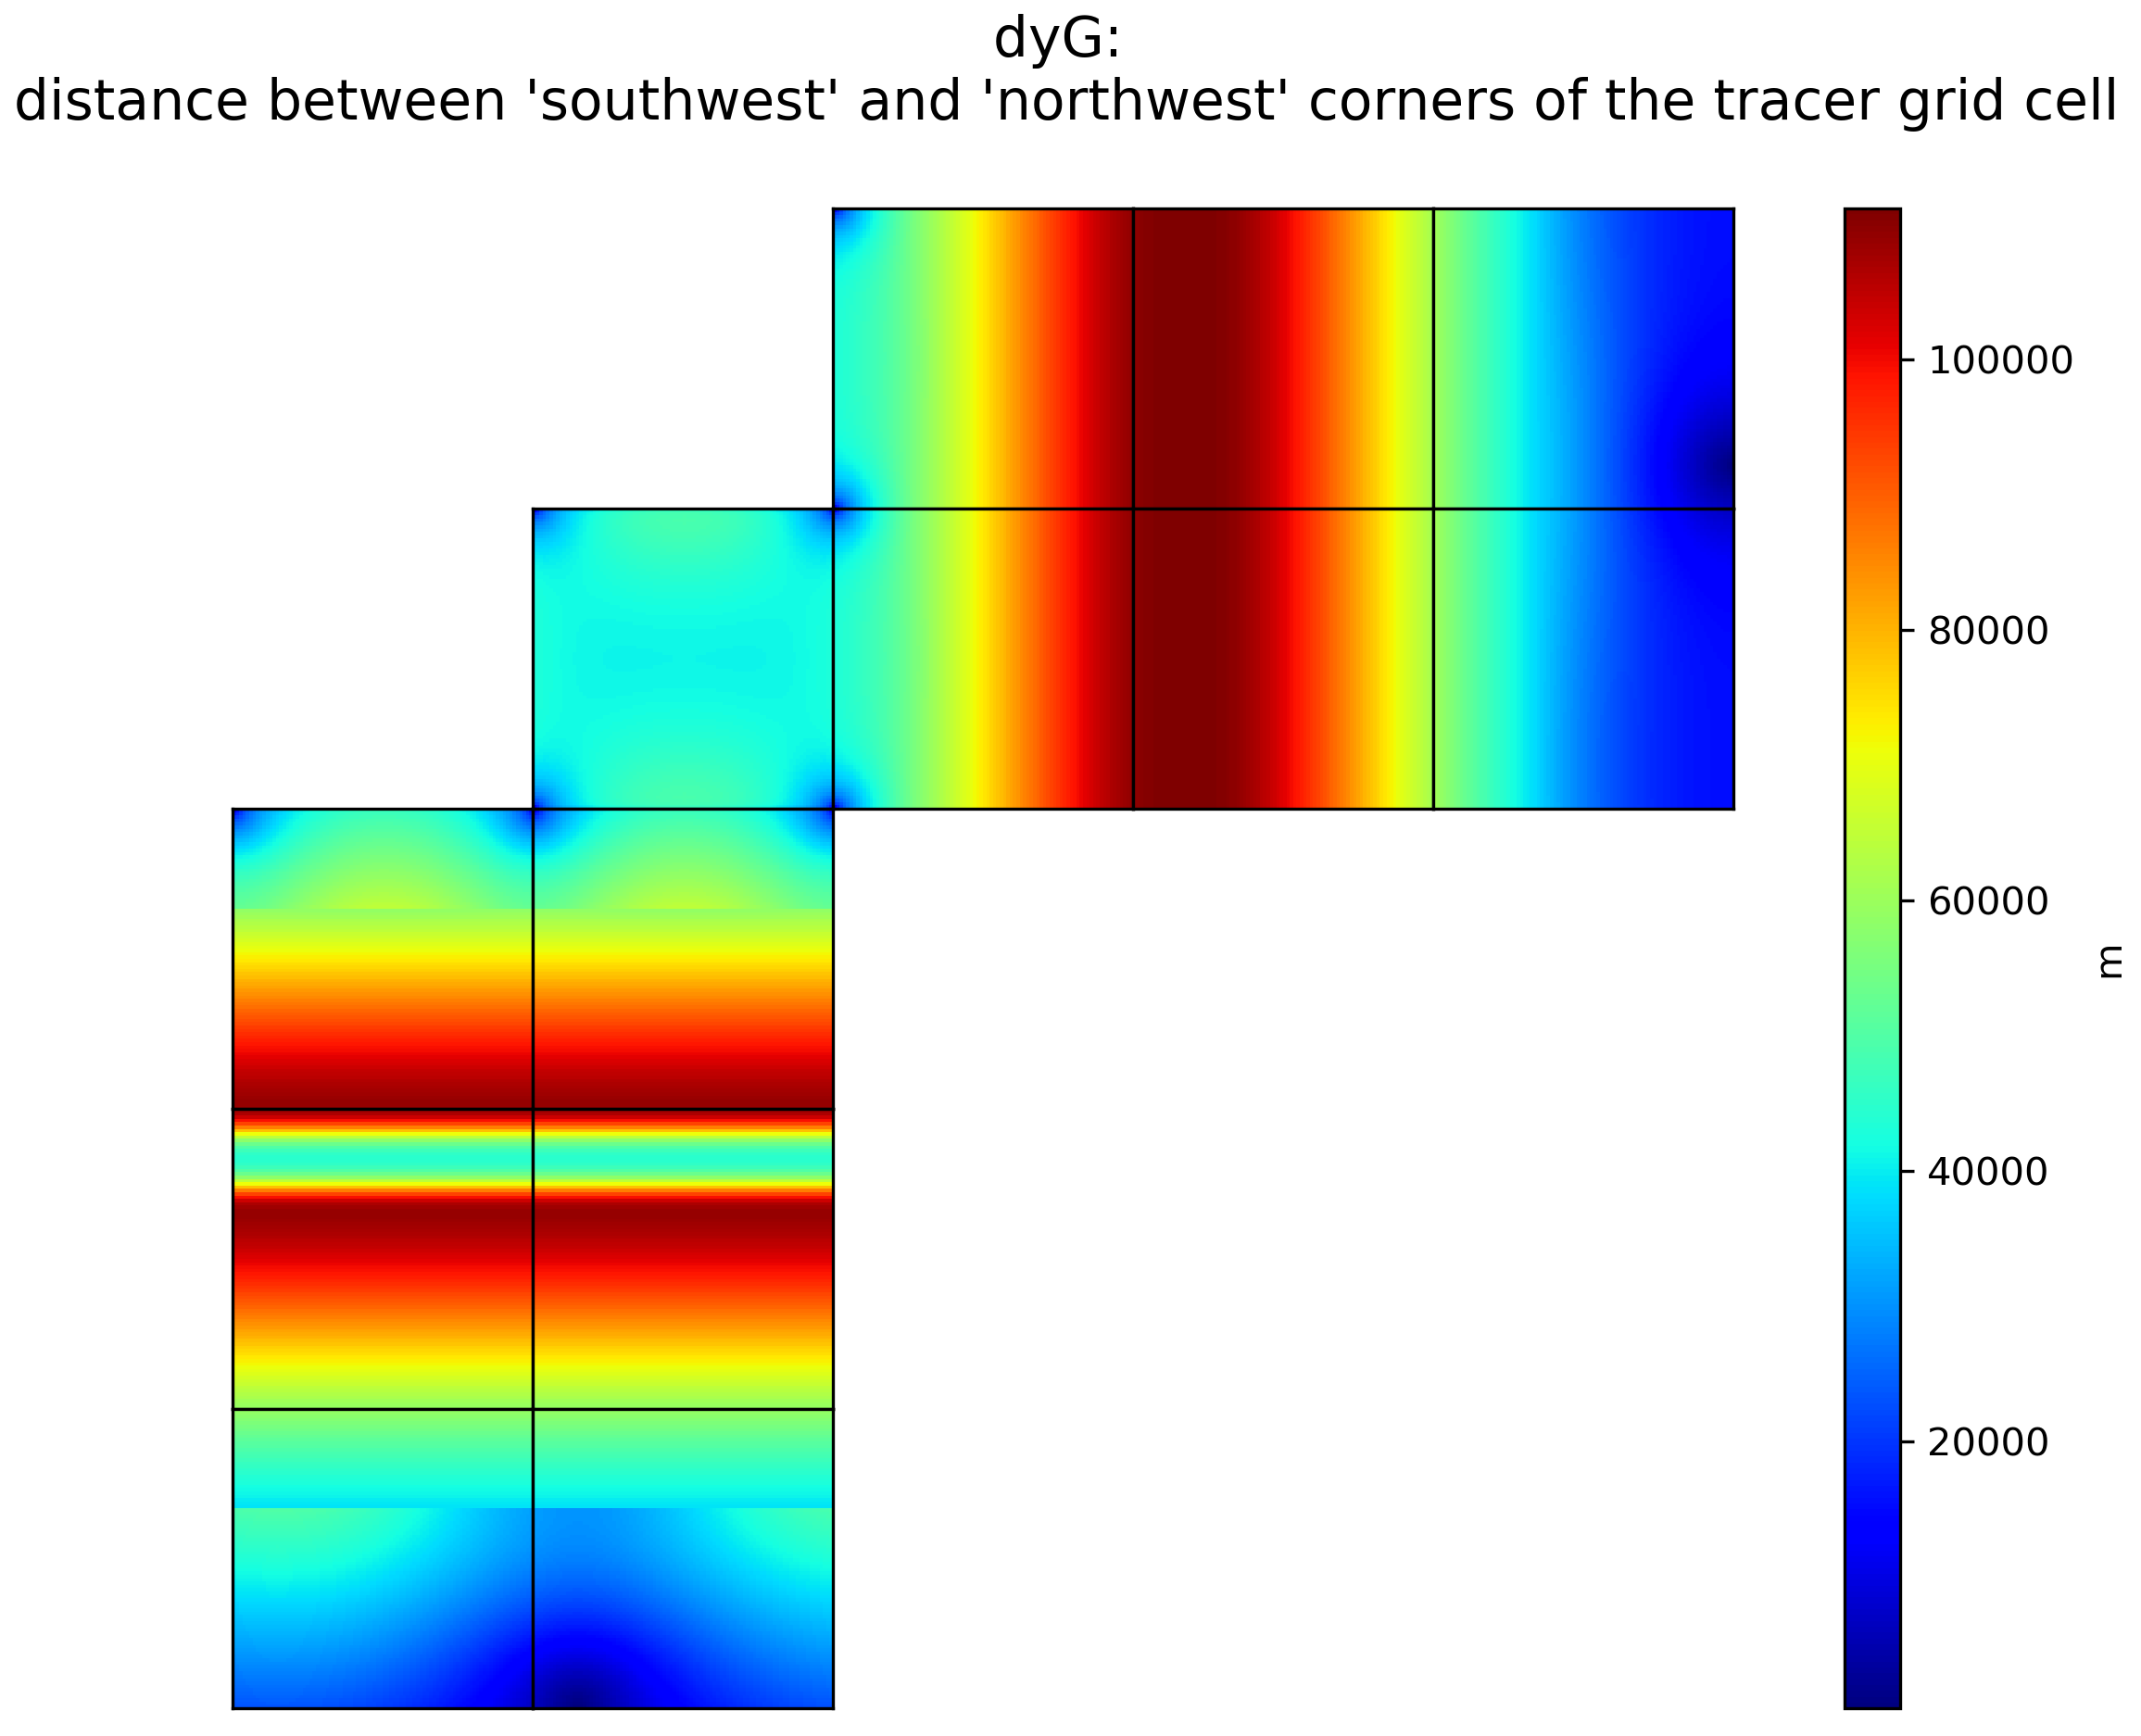
\includegraphics[scale=0.5]{../images/plots/native_plots_coords/Geometry_Parameters_for_the_Lat-Lon-Cap_90_(llc90)_Native_Model_Grid_(Version_4_Release_4)/dyG.png}
\caption{\\Dataset: GRID\_GEOMETRY\_ECCO\\Variable: dyG}
\label{tab:table-GRID_GEOMETRY_ECCO_dyG-Plot}
\end{figure}
\pagebreak
\subsubsection{Native coordinates Variable Depth}
\begin{longtable}{|p{0.06\textwidth}|p{0.41\textwidth}|p{0.39\textwidth}|p{0.06\textwidth}|}
    \caption{CDL description of GRID\_GEOMETRY\_ECCO's Depth variable}
    \label{tab:table-GRID_GEOMETRY_ECCO_Depth} \\ 
    \hline \endhead \hline \endfoot
    \rowcolor{lightgray} \textbf{Storage Type} & \textbf{Variable Name} & \textbf{Description} & \textbf{Unit} \\ \hline
    float32 & Depth & model seafloor depth below ocean surface at rest & m \\ \hline
    \rowcolor{lightgray}  \multicolumn{4}{|p{1.00\textwidth}|}{\textbf{CDL Description}} \\ \hline
    \multicolumn{4}{|p{1.00\textwidth}|}{\makecell{\parbox{1\textwidth}{float32 Depth(tile, j, i)\\
    \hspace*{0.5cm}Depth: \_FillValue = 9.96921e+36\\
    \hspace*{0.5cm}Depth: long\_name = model seafloor depth below ocean surface at rest\\
    \hspace*{0.5cm}Depth: units = m\\
    \hspace*{0.5cm}Depth: coordinate = XC YC\\
    \hspace*{0.5cm}Depth: coverage\_content\_type = modelResult\\
    \hspace*{0.5cm}Depth: standard\_name = sea\_floor\_depth\_below\_geoid\\
    \hspace*{0.5cm}Depth: coordinates = YC XC}}} \\ \hline
    \rowcolor{lightgray} \multicolumn{4}{|p{1.00\textwidth}|}{\textbf{Comments}} \\ \hline
    \multicolumn{4}{|p{1\textwidth}|}{Model sea surface height (SSH) of 0m corresponds to an ocean surface at rest relative to the geoid. Depth corresponds to seafloor depth below geoid. Note: the MITgcm used by ECCO V4r4 implements 'partial cells' so the actual model seafloor depth may differ from the seafloor depth provided by the input bathymetry file.} \\ \hline
\end{longtable}

\begin{figure}[H]
\centering
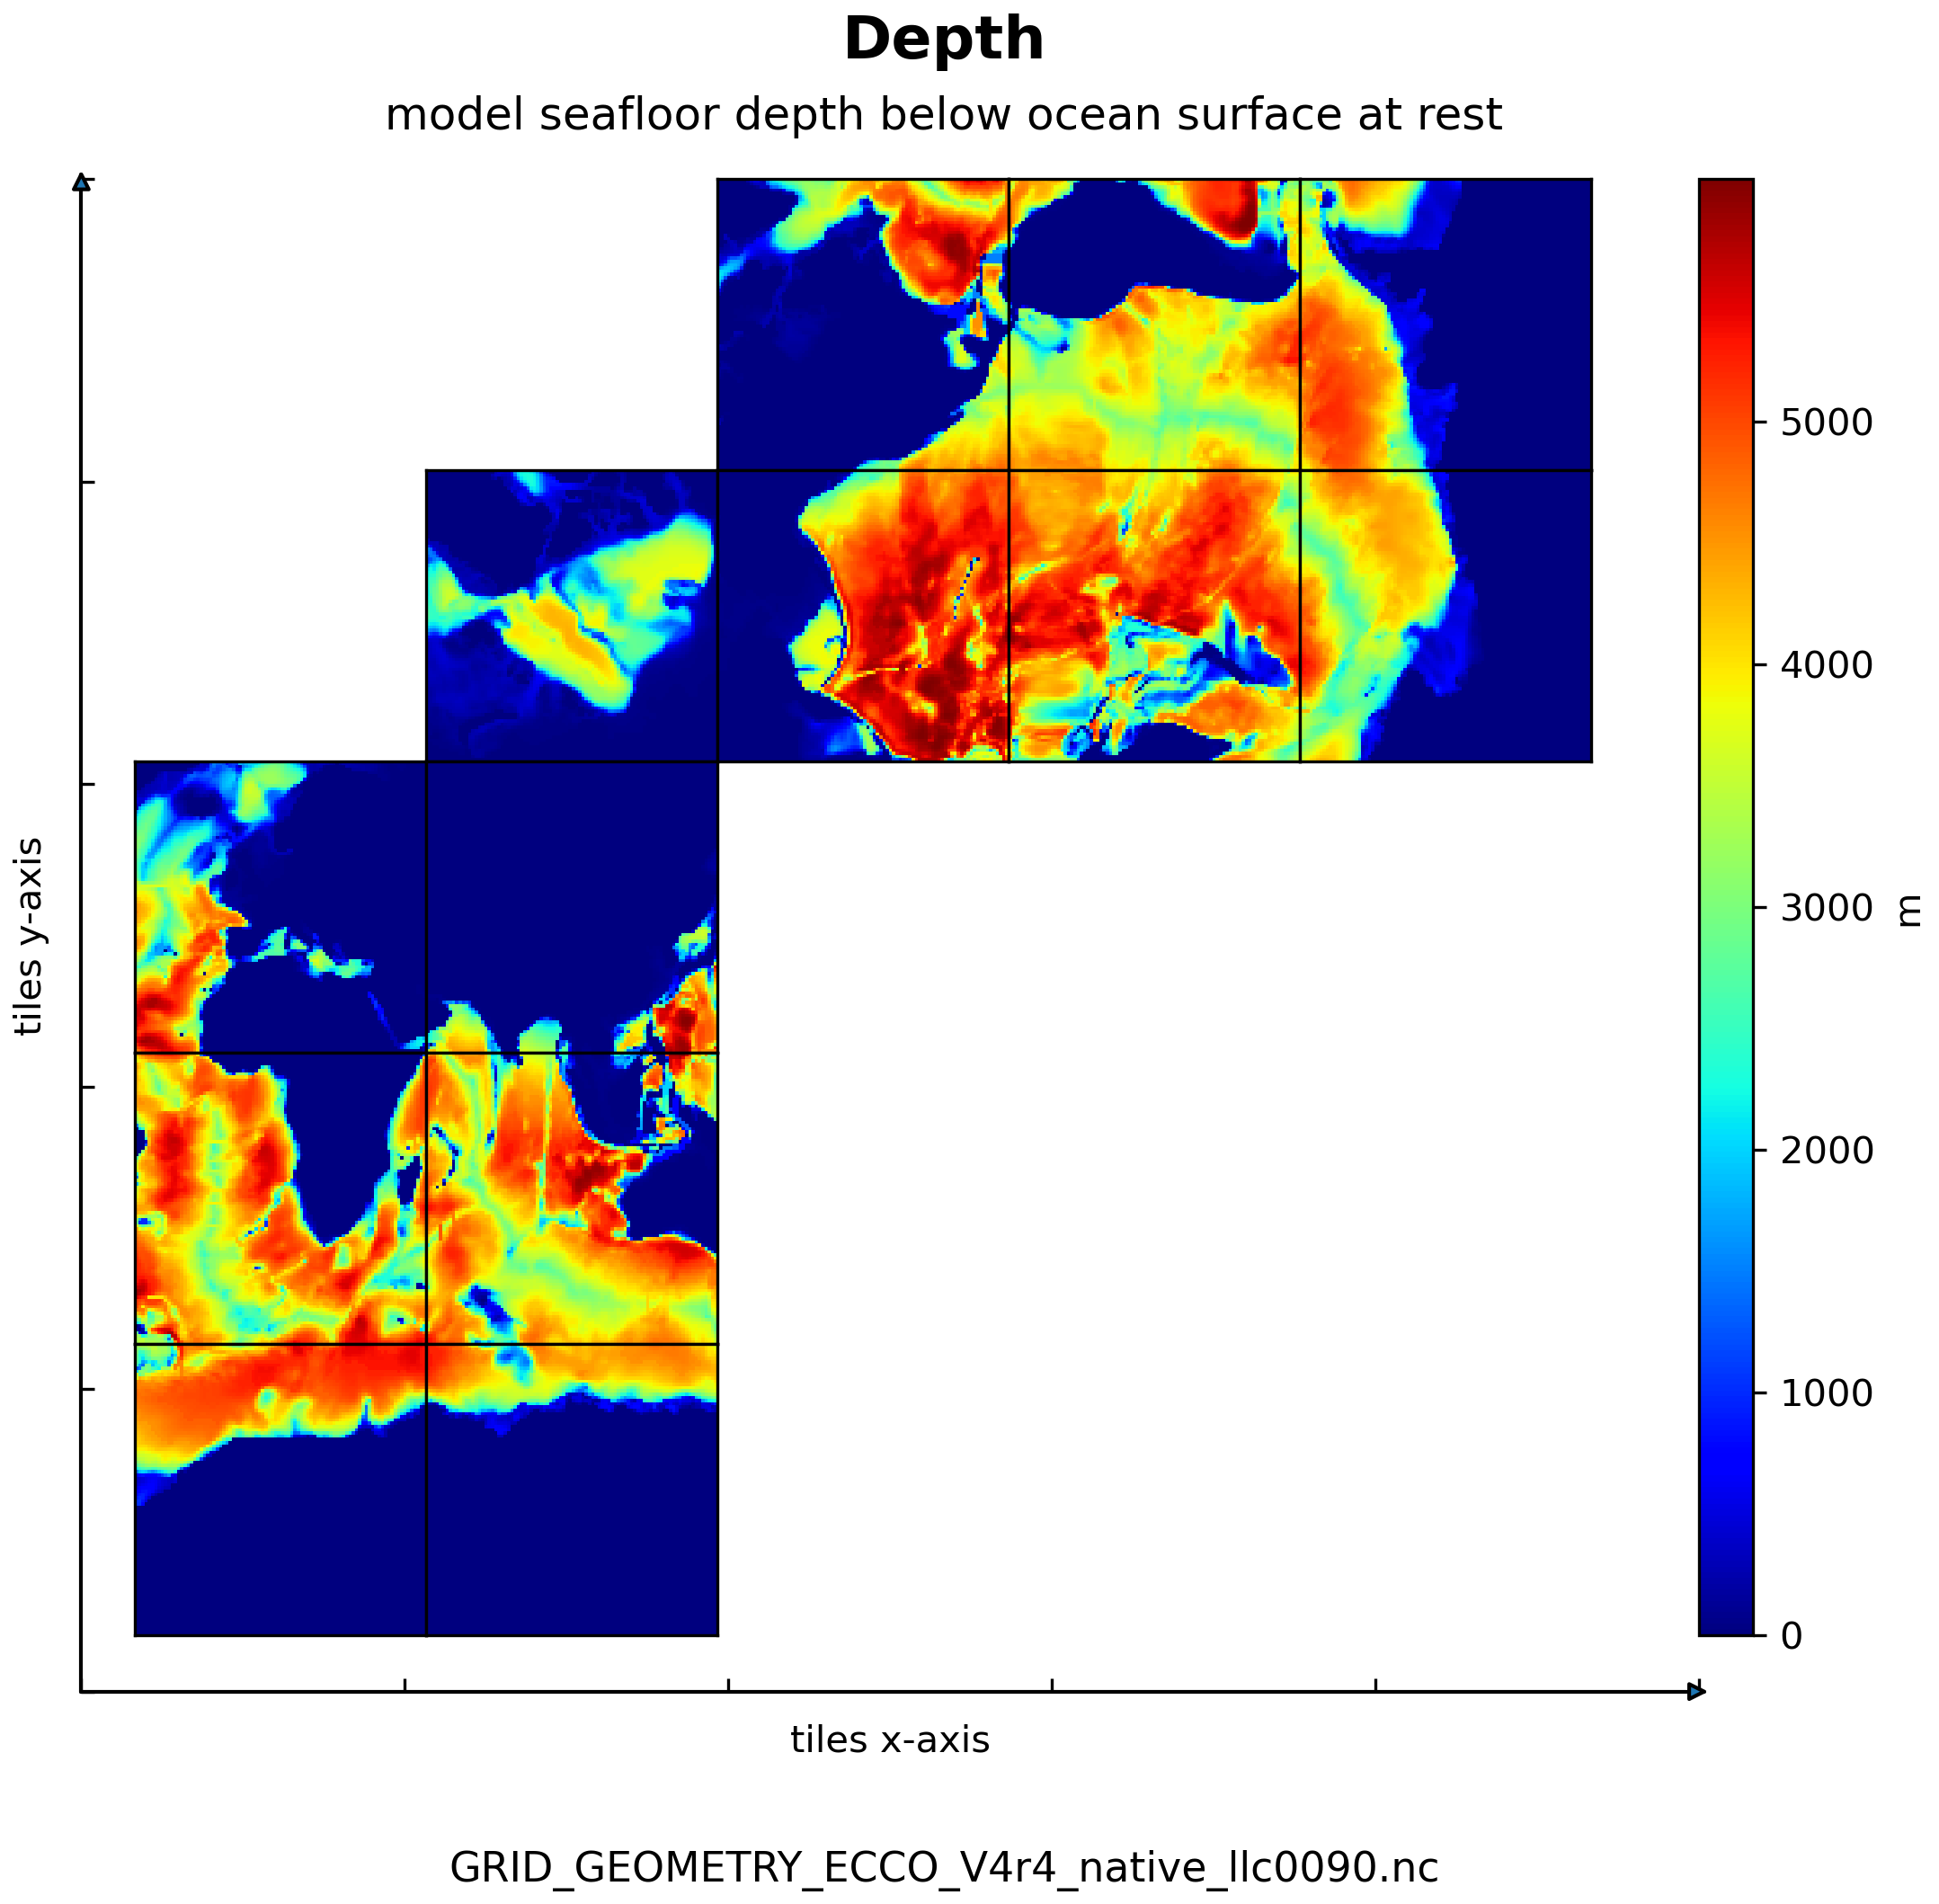
\includegraphics[scale=0.5]{../images/plots/native_plots_coords/Geometry_Parameters_for_the_Lat-Lon-Cap_90_(llc90)_Native_Model_Grid_(Version_4_Release_4)/Depth.png}
\caption{\\Dataset: GRID\_GEOMETRY\_ECCO\\Variable: Depth}
\label{tab:table-GRID_GEOMETRY_ECCO_Depth-Plot}
\end{figure}
\pagebreak
\subsubsection{Native coordinates Variable rAz}
\begin{longtable}{|p{0.06\textwidth}|p{0.41\textwidth}|p{0.39\textwidth}|p{0.06\textwidth}|}
    \caption{CDL description of GRID\_GEOMETRY\_ECCO's rAz variable}
    \label{tab:table-GRID_GEOMETRY_ECCO_rAz} \\ 
    \hline \endhead \hline \endfoot
    \rowcolor{lightgray} \textbf{Storage Type} & \textbf{Variable Name} & \textbf{Description} & \textbf{Unit} \\ \hline
    float32 & rAz & area of vorticity 'g' grid cell & m2 \\ \hline
    \rowcolor{lightgray}  \multicolumn{4}{|p{1.00\textwidth}|}{\textbf{CDL Description}} \\ \hline
    \multicolumn{4}{|p{1.00\textwidth}|}{\makecell{\parbox{1\textwidth}{float32 rAz(tile, j\_g, i\_g)\\
    \hspace*{0.5cm}rAz: \_FillValue = 9.96921e+36\\
    \hspace*{0.5cm}rAz: long\_name = "area of vorticity g grid cell"\\
    \hspace*{0.5cm}rAz: units = m2\\
    \hspace*{0.5cm}rAz: coordinate = YG XG\\
    \hspace*{0.5cm}rAz: coverage\_content\_type = modelResult\\
    \hspace*{0.5cm}rAz: standard\_name = cell\_area\\
    \hspace*{0.5cm}rAz: coordinates = YG XG}}} \\ \hline
    \rowcolor{lightgray} \multicolumn{4}{|p{1.00\textwidth}|}{\textbf{Comments}} \\ \hline
    \multicolumn{4}{|p{1\textwidth}|}{Vorticity cells are staggered in space relative to tracer cells, nominally situated on tracer cell corners. Vorticity cell (i,j) is located at the 'southwest' corner of tracer grid cell (i, j). Note: 'southwest' does not correspond to geographic orientation but is used for convenience to describe the computational grid. See MITgcm documentation for details.} \\ \hline
\end{longtable}

\begin{figure}[H]
\centering
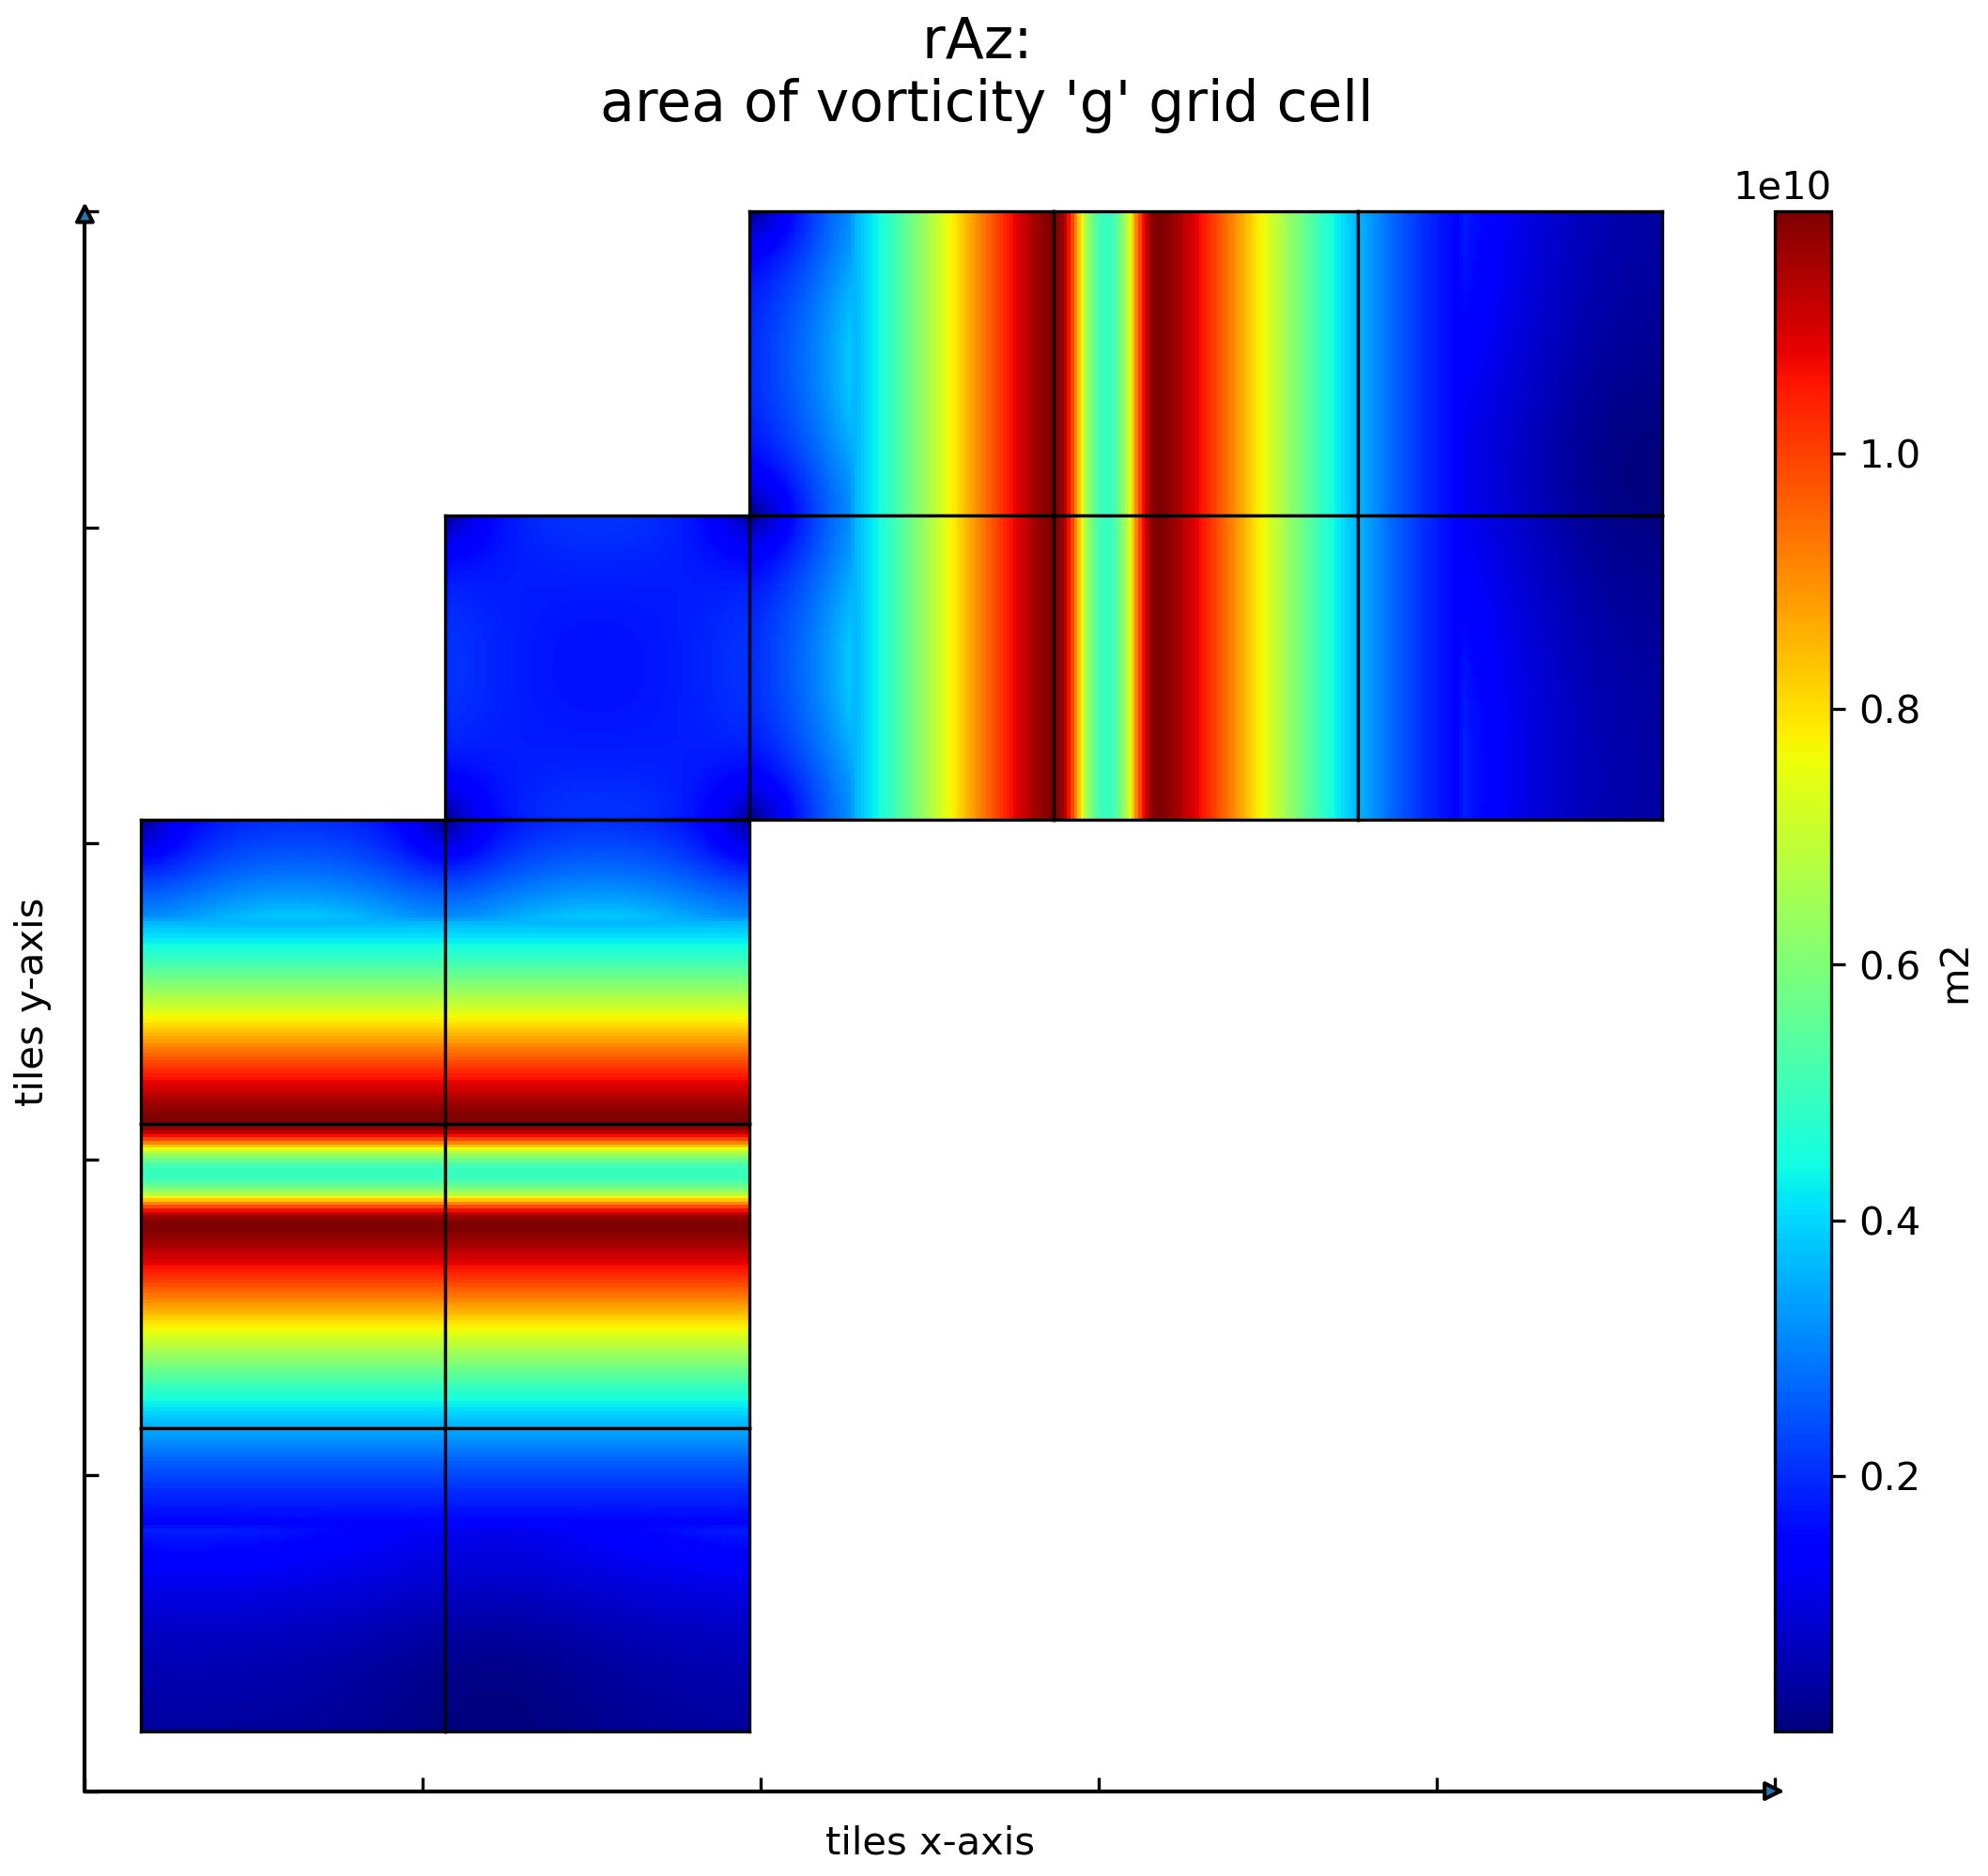
\includegraphics[scale=0.5]{../images/plots/native_plots_coords/Geometry_Parameters_for_the_Lat-Lon-Cap_90_(llc90)_Native_Model_Grid_(Version_4_Release_4)/rAz.png}
\caption{\\Dataset: GRID\_GEOMETRY\_ECCO\\Variable: rAz}
\label{tab:table-GRID_GEOMETRY_ECCO_rAz-Plot}
\end{figure}
\pagebreak
\subsubsection{Native coordinates Variable dxC}
    \begin{longtable}{|p{0.06\textwidth}|p{0.41\textwidth}|p{0.39\textwidth}|p{0.06\textwidth}|}
    \caption{CDL description of GRID\_GEOMETRY\_ECCO's dxC variable}
    \label{tab:table-GRID_GEOMETRY_ECCO_dxC} \\ 
    \hline \endhead \hline \endfoot
    \rowcolor{lightgray} \textbf{Storage Type} & \textbf{Variable Name} & \textbf{Description} & \textbf{Unit} \\ \hline
    float32 & dxC & distance between centers of adjacent tracer grid cells in the 'x' direction & m \\ \hline
    \rowcolor{lightgray}  \multicolumn{4}{|p{1.00\textwidth}|}{\textbf{CDL Description}} \\ \hline
    \multicolumn{4}{|p{1.00\textwidth}|}{\makecell{\parbox{1\textwidth}{float32 dxC(tile, j, i\_g)\\
    \hspace*{0.5cm}dxC: \_FillValue = 9.96921e+36\\
    \hspace*{0.5cm}dxC: long\_name = "distance between centers of adjacent tracer grid cells in the x direction"\\
    \hspace*{0.5cm}dxC: units = m\\
    \hspace*{0.5cm}dxC: coordinate = YC XG\\
    \hspace*{0.5cm}dxC: coverage\_content\_type = modelResult}}} \\ \hline
    \rowcolor{lightgray} \multicolumn{4}{|p{1.00\textwidth}|}{\textbf{Comments}} \\ \hline
    \multicolumn{4}{|p{1\textwidth}|}{Alternatively, the length of 'north' side of vorticity grid cells. Note: 'north' does not correspond to geographic orientation but is used for convenience to describe the computational grid. See MITgcm documentation for details.} \\ \hline
\end{longtable}

\begin{figure}[H]
\centering
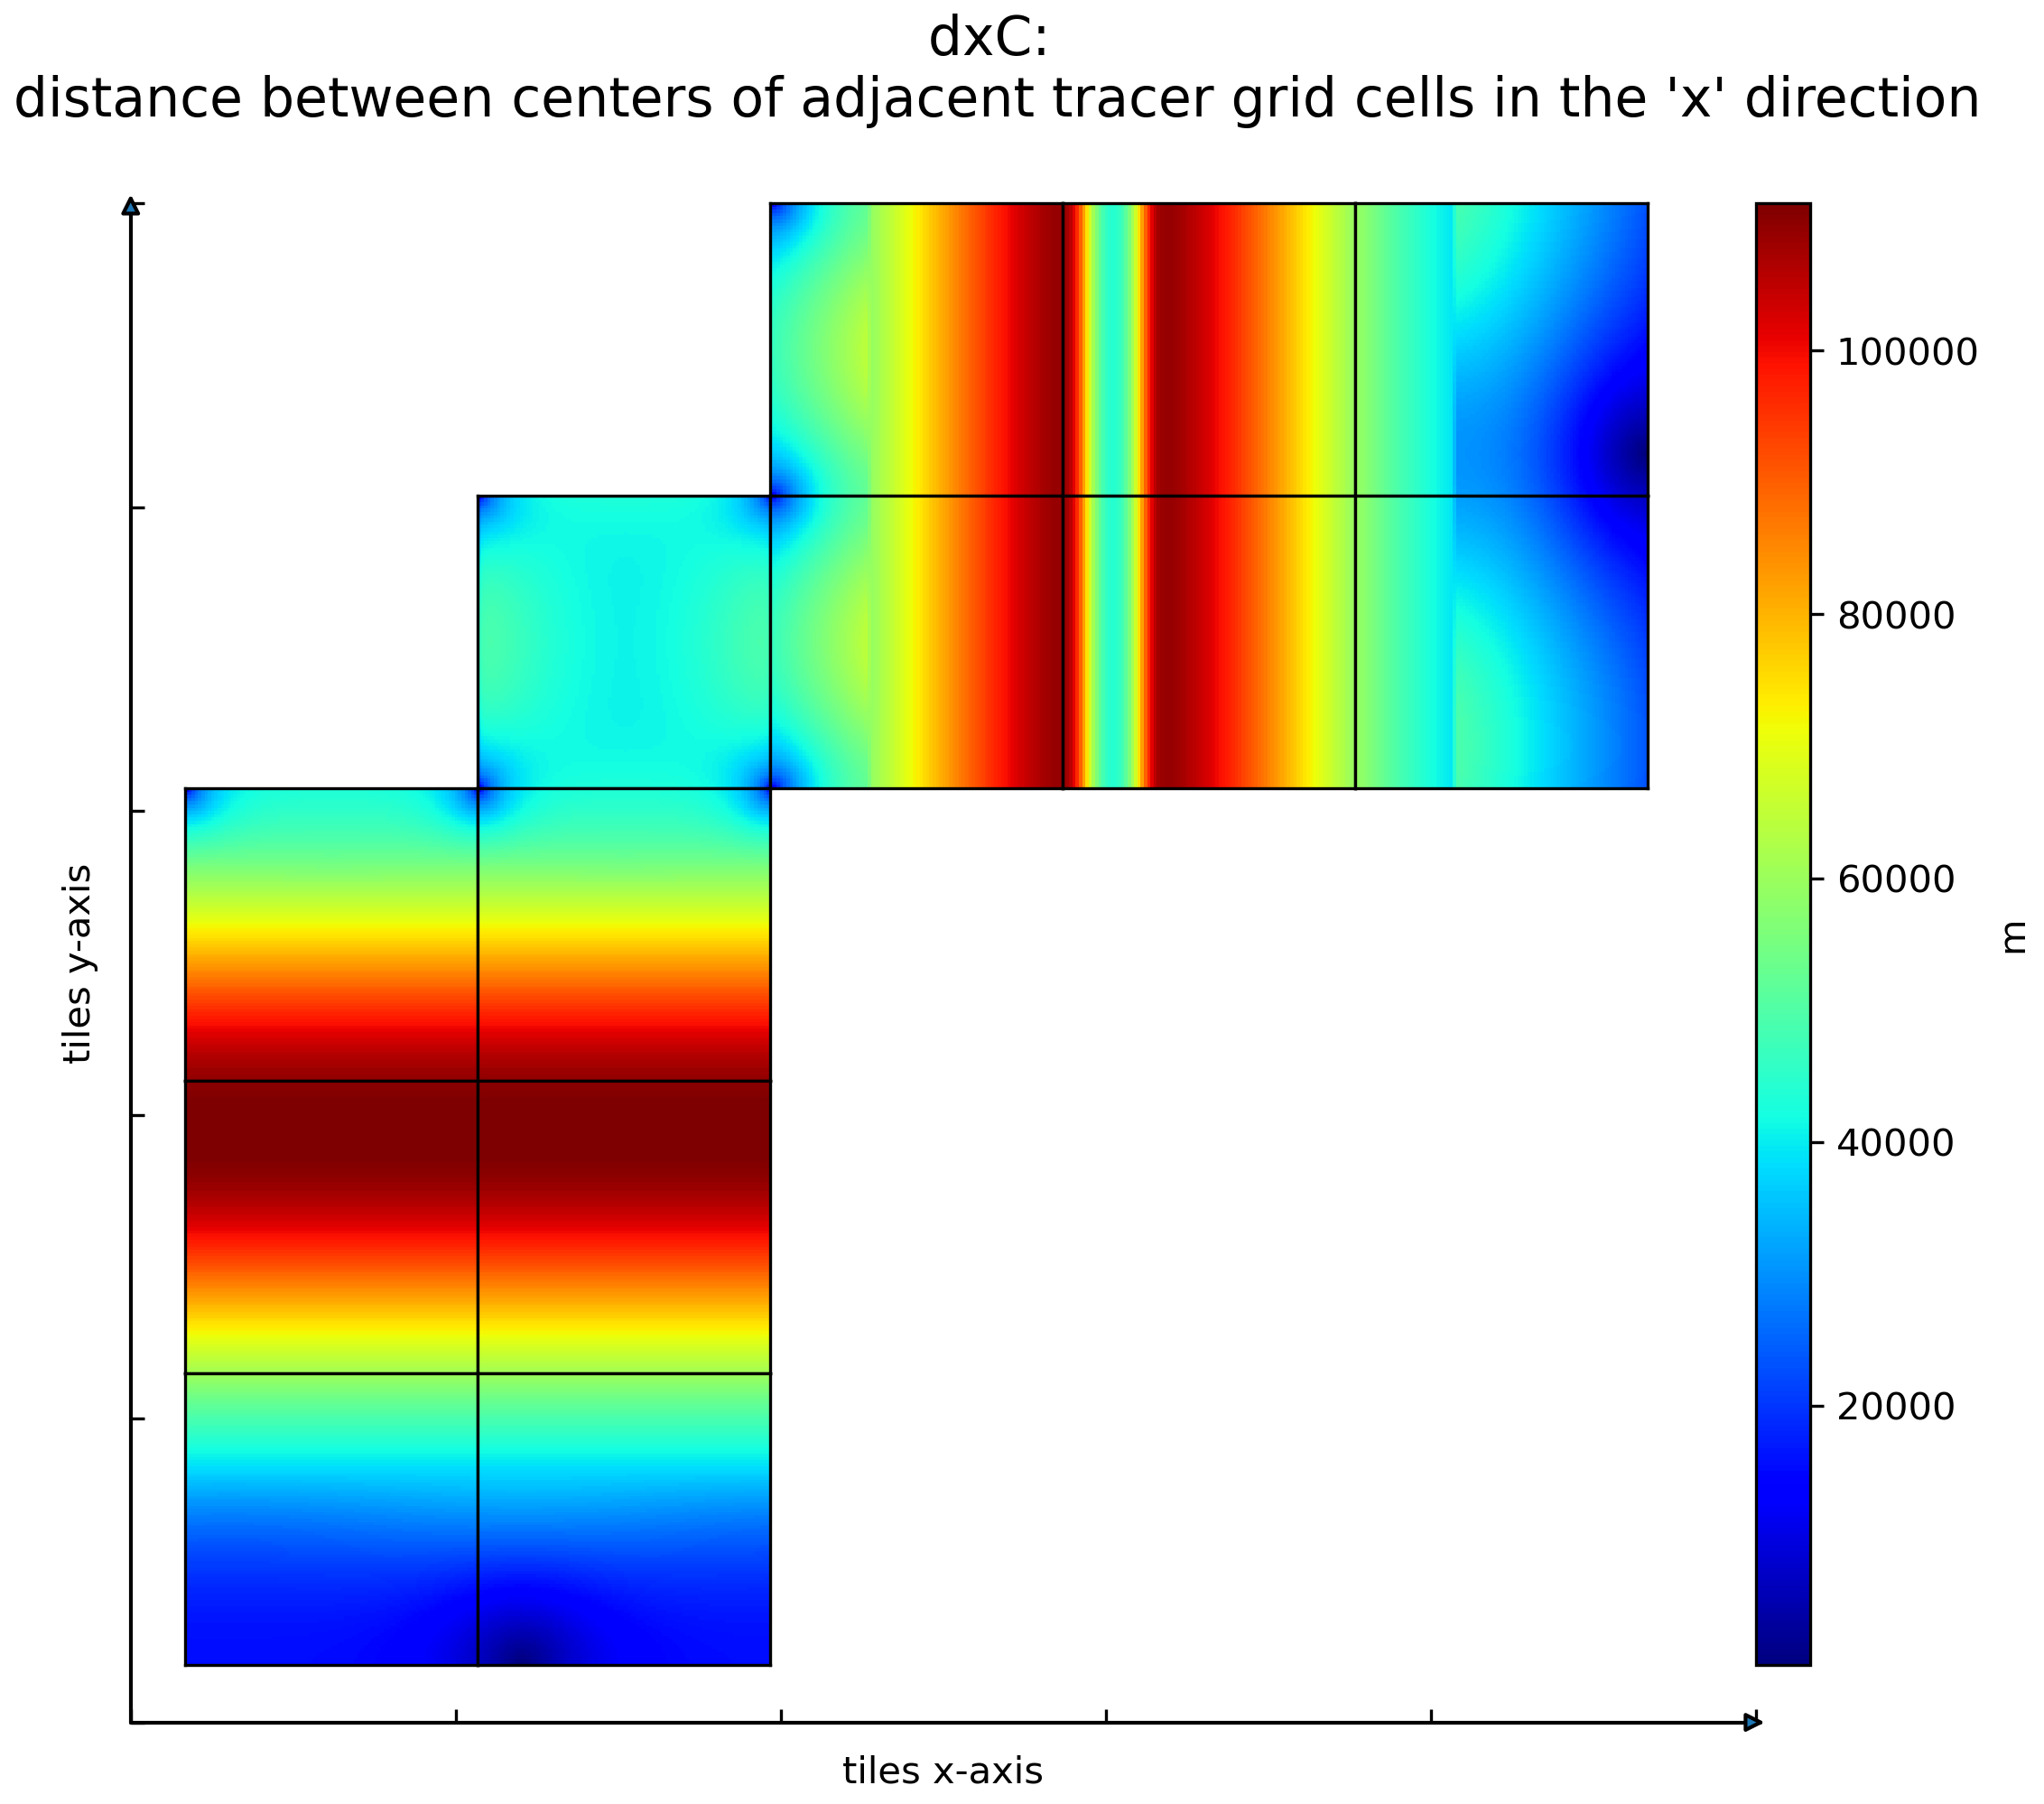
\includegraphics[scale=0.5]{../images/plots/native_plots_coords/Geometry_Parameters_for_the_Lat-Lon-Cap_90_(llc90)_Native_Model_Grid_(Version_4_Release_4)/dxC.png}
\caption{\\Dataset: GRID\_GEOMETRY\_ECCO\\Variable: dxC}
\label{tab:table-GRID_GEOMETRY_ECCO_dxC-Plot}
\end{figure}
\pagebreak
\subsubsection{Native coordinates Variable dyC}
\begin{longtable}{|p{0.06\textwidth}|p{0.41\textwidth}|p{0.39\textwidth}|p{0.06\textwidth}|}
    \caption{CDL description of GRID\_GEOMETRY\_ECCO's dyC variable}
    \label{tab:table-GRID_GEOMETRY_ECCO_dyC} \\ 
    \hline \endhead \hline \endfoot
    \rowcolor{lightgray} \textbf{Storage Type} & \textbf{Variable Name} & \textbf{Description} & \textbf{Unit} \\ \hline
    float32 & dyC & distance between centers of adjacent tracer grid cells in the 'y' direction & m \\ \hline
    \rowcolor{lightgray}  \multicolumn{4}{|p{1.00\textwidth}|}{\textbf{CDL Description}} \\ \hline
    \multicolumn{4}{|p{1.00\textwidth}|}{\makecell{\parbox{1\textwidth}{float32 dyC(tile, j\_g, i)\\
    \hspace*{0.5cm}dyC: \_FillValue = 9.96921e+36\\
    \hspace*{0.5cm}dyC: long\_name = "distance between centers of adjacent tracer grid cells in the y direction"\\
    \hspace*{0.5cm}dyC: units = m\\
    \hspace*{0.5cm}dyC: coordinate = YG XC\\
    \hspace*{0.5cm}dyC: coverage\_content\_type = modelResult}}} \\ \hline
    \rowcolor{lightgray} \multicolumn{4}{|p{1.00\textwidth}|}{\textbf{Comments}} \\ \hline
    \multicolumn{4}{|p{1\textwidth}|}{Alternatively, the length of 'east' side of vorticity grid cells. Note: 'east' does not correspond to geographic orientation but is used for convenience to describe the computational grid. See MITgcm documentation for details.} \\ \hline
\end{longtable}

\begin{figure}[H]
\centering
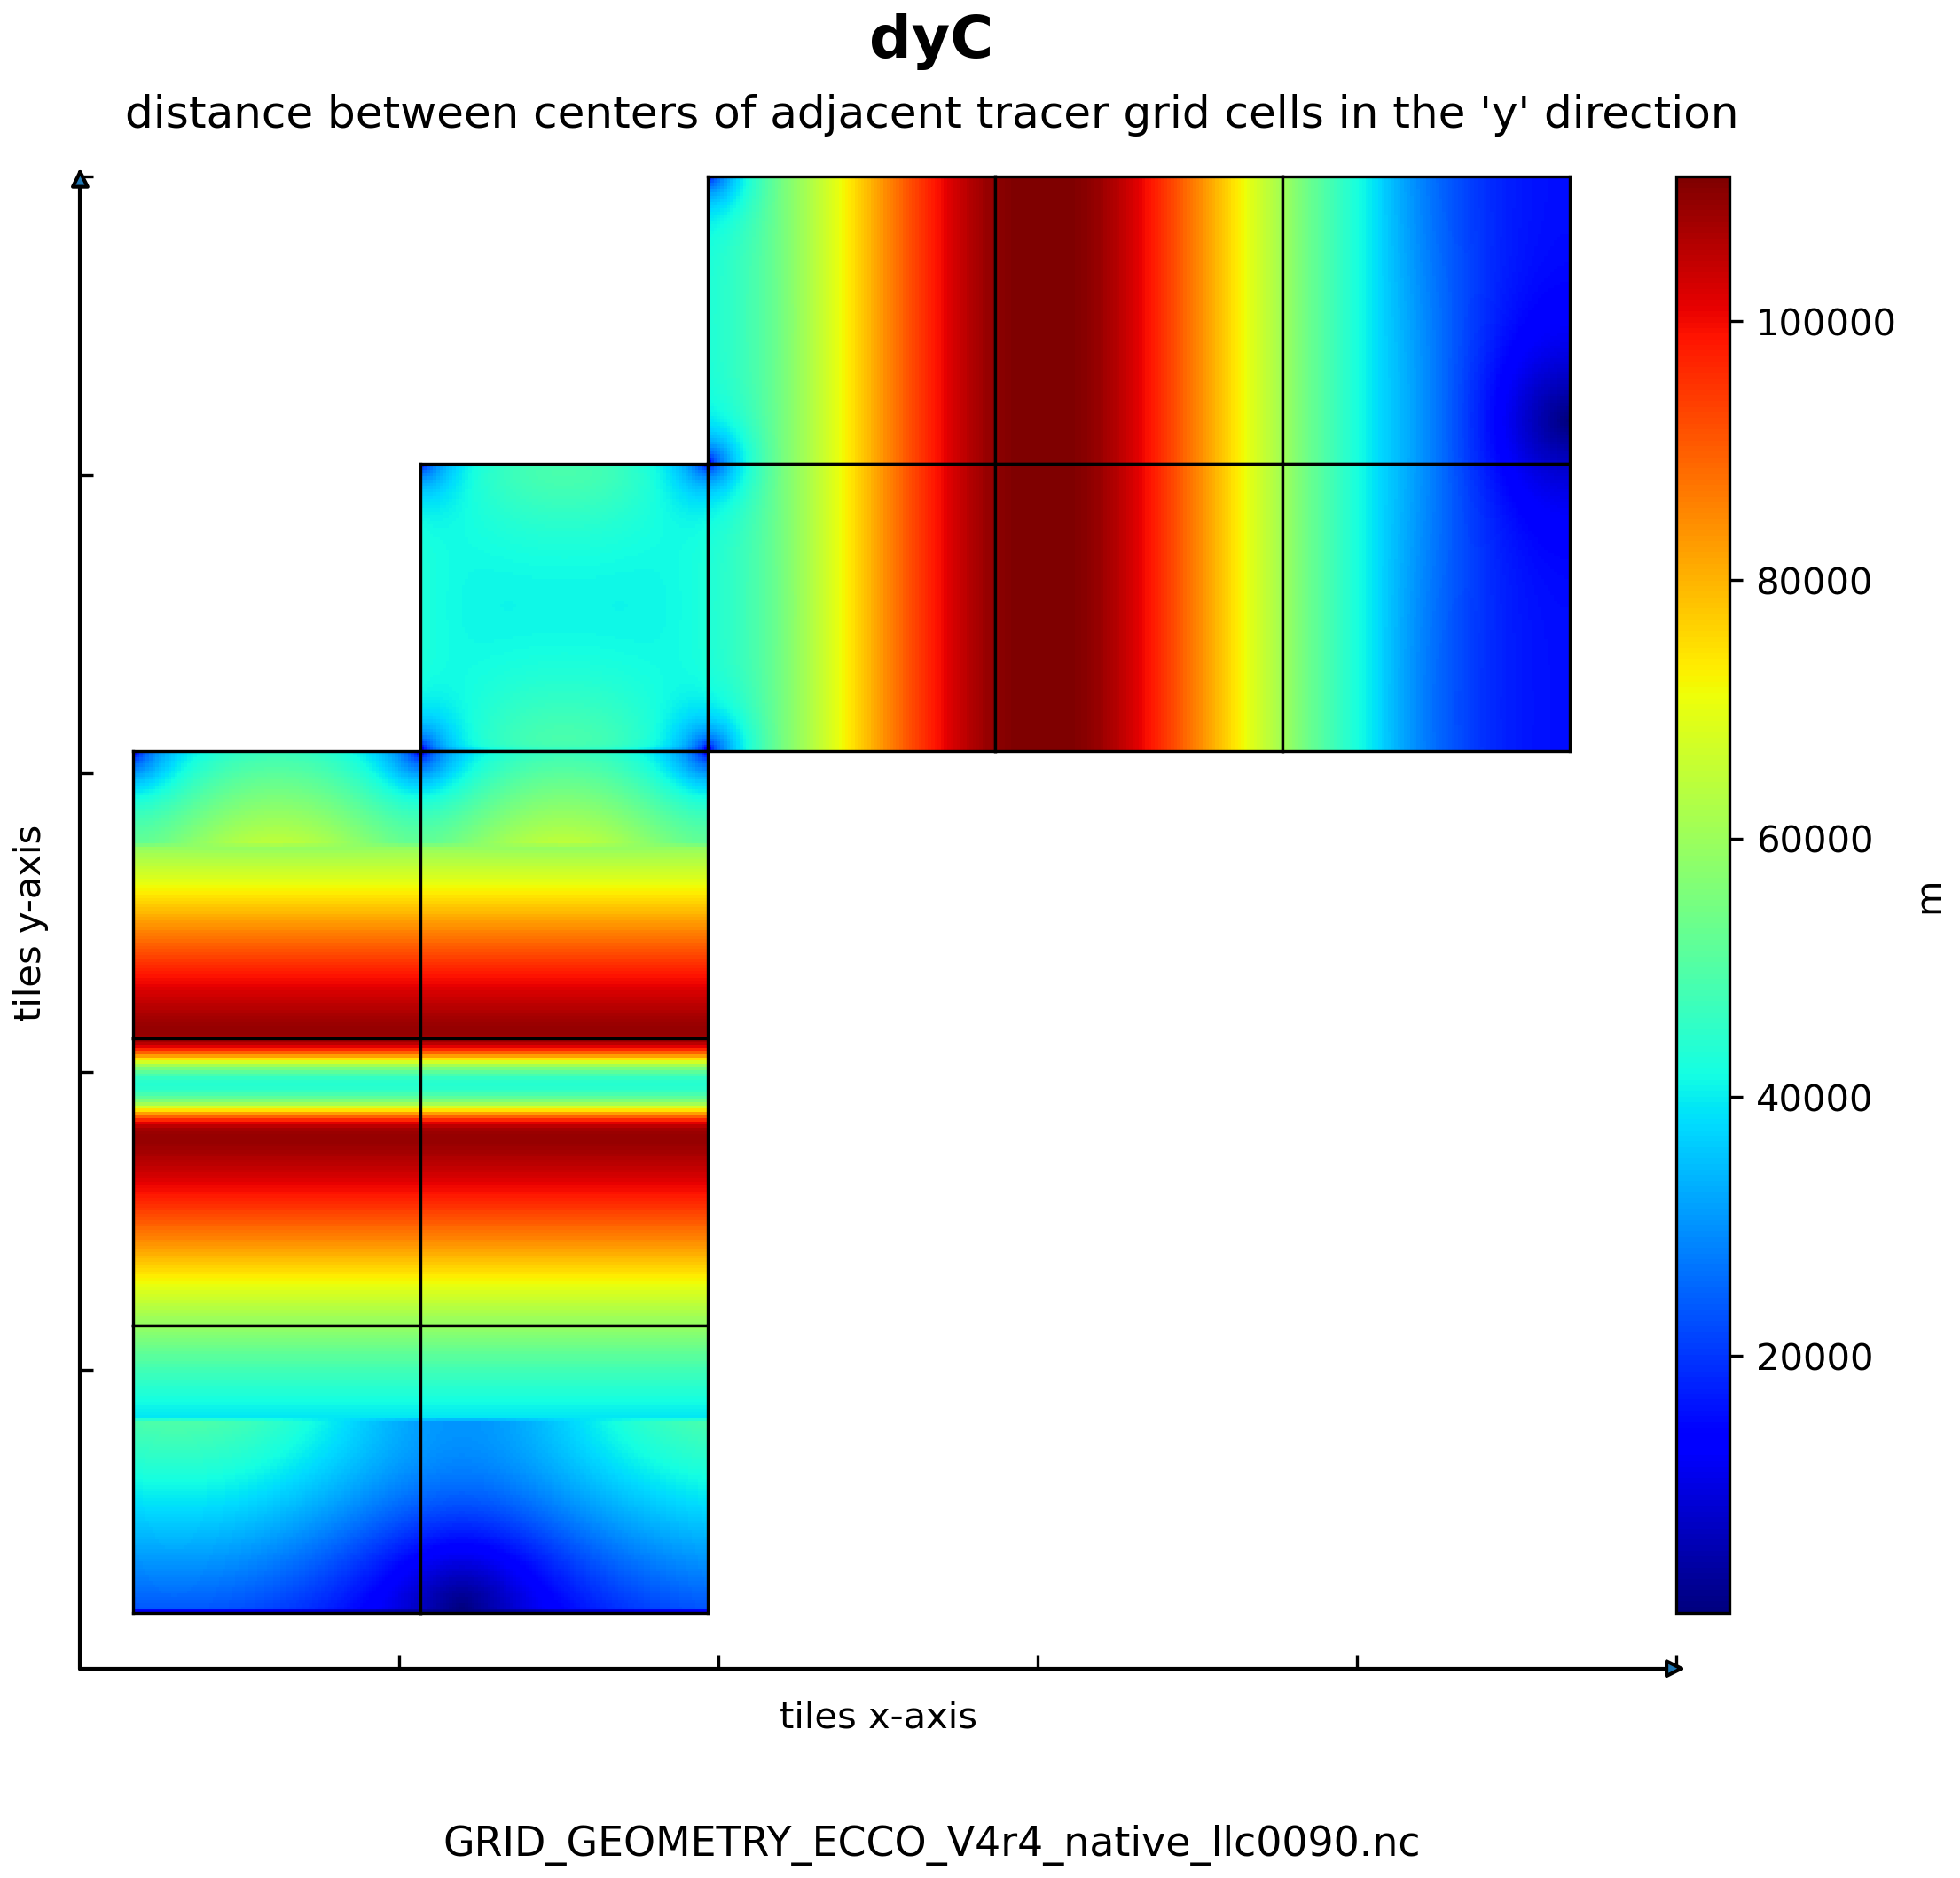
\includegraphics[scale=0.5]{../images/plots/native_plots_coords/Geometry_Parameters_for_the_Lat-Lon-Cap_90_(llc90)_Native_Model_Grid_(Version_4_Release_4)/dyC.png}
\caption{\\Dataset: GRID\_GEOMETRY\_ECCO\\Variable: dyC}
\label{tab:table-GRID_GEOMETRY_ECCO_dyC-Plot}
\end{figure}
\pagebreak
\subsubsection{Native coordinates Variable rAw}
\begin{longtable}{|p{0.06\textwidth}|p{0.41\textwidth}|p{0.39\textwidth}|p{0.06\textwidth}|}
    \caption{CDL description of GRID\_GEOMETRY\_ECCO's rAw variable}
    \label{tab:table-GRID_GEOMETRY_ECCO_rAw} \\ 
    \hline \endhead \hline \endfoot
    \rowcolor{lightgray} \textbf{Storage Type} & \textbf{Variable Name} & \textbf{Description} & \textbf{Unit} \\ \hline
    float32 & rAw & area of 'v' grid cell & m2 \\ \hline
    \rowcolor{lightgray}  \multicolumn{4}{|p{1.00\textwidth}|}{\textbf{CDL Description}} \\ \hline
    \multicolumn{4}{|p{1.00\textwidth}|}{\makecell{\parbox{1\textwidth}{float32 rAw(tile, j, i\_g)\\
    \hspace*{0.5cm}rAw: \_FillValue = 9.96921e+36\\
    \hspace*{0.5cm}rAw: long\_name = "area of v grid cell"\\
    \hspace*{0.5cm}rAw: units = m2\\
    \hspace*{0.5cm}rAw: coordinate = YG XC\\
    \hspace*{0.5cm}rAw: coverage\_content\_type = modelResult\\
    \hspace*{0.5cm}rAw: standard\_name = cell\_area}}} \\ \hline
    \rowcolor{lightgray} \multicolumn{4}{|p{1.00\textwidth}|}{\textbf{Comments}} \\ \hline
    \multicolumn{4}{|p{1\textwidth}|}{Model 'v' grid cells are staggered in space between adjacent tracer grid cells in the 'x' direction. 'v' grid cell (i,j) is situated at the 'west' edge of tracer grid cell (i, j). Note: 'west' does not correspond to geographic orientation but is used for convenience to describe the computational grid. See MITgcm documentation for details.} \\ \hline
\end{longtable}

\begin{figure}[H]
\centering
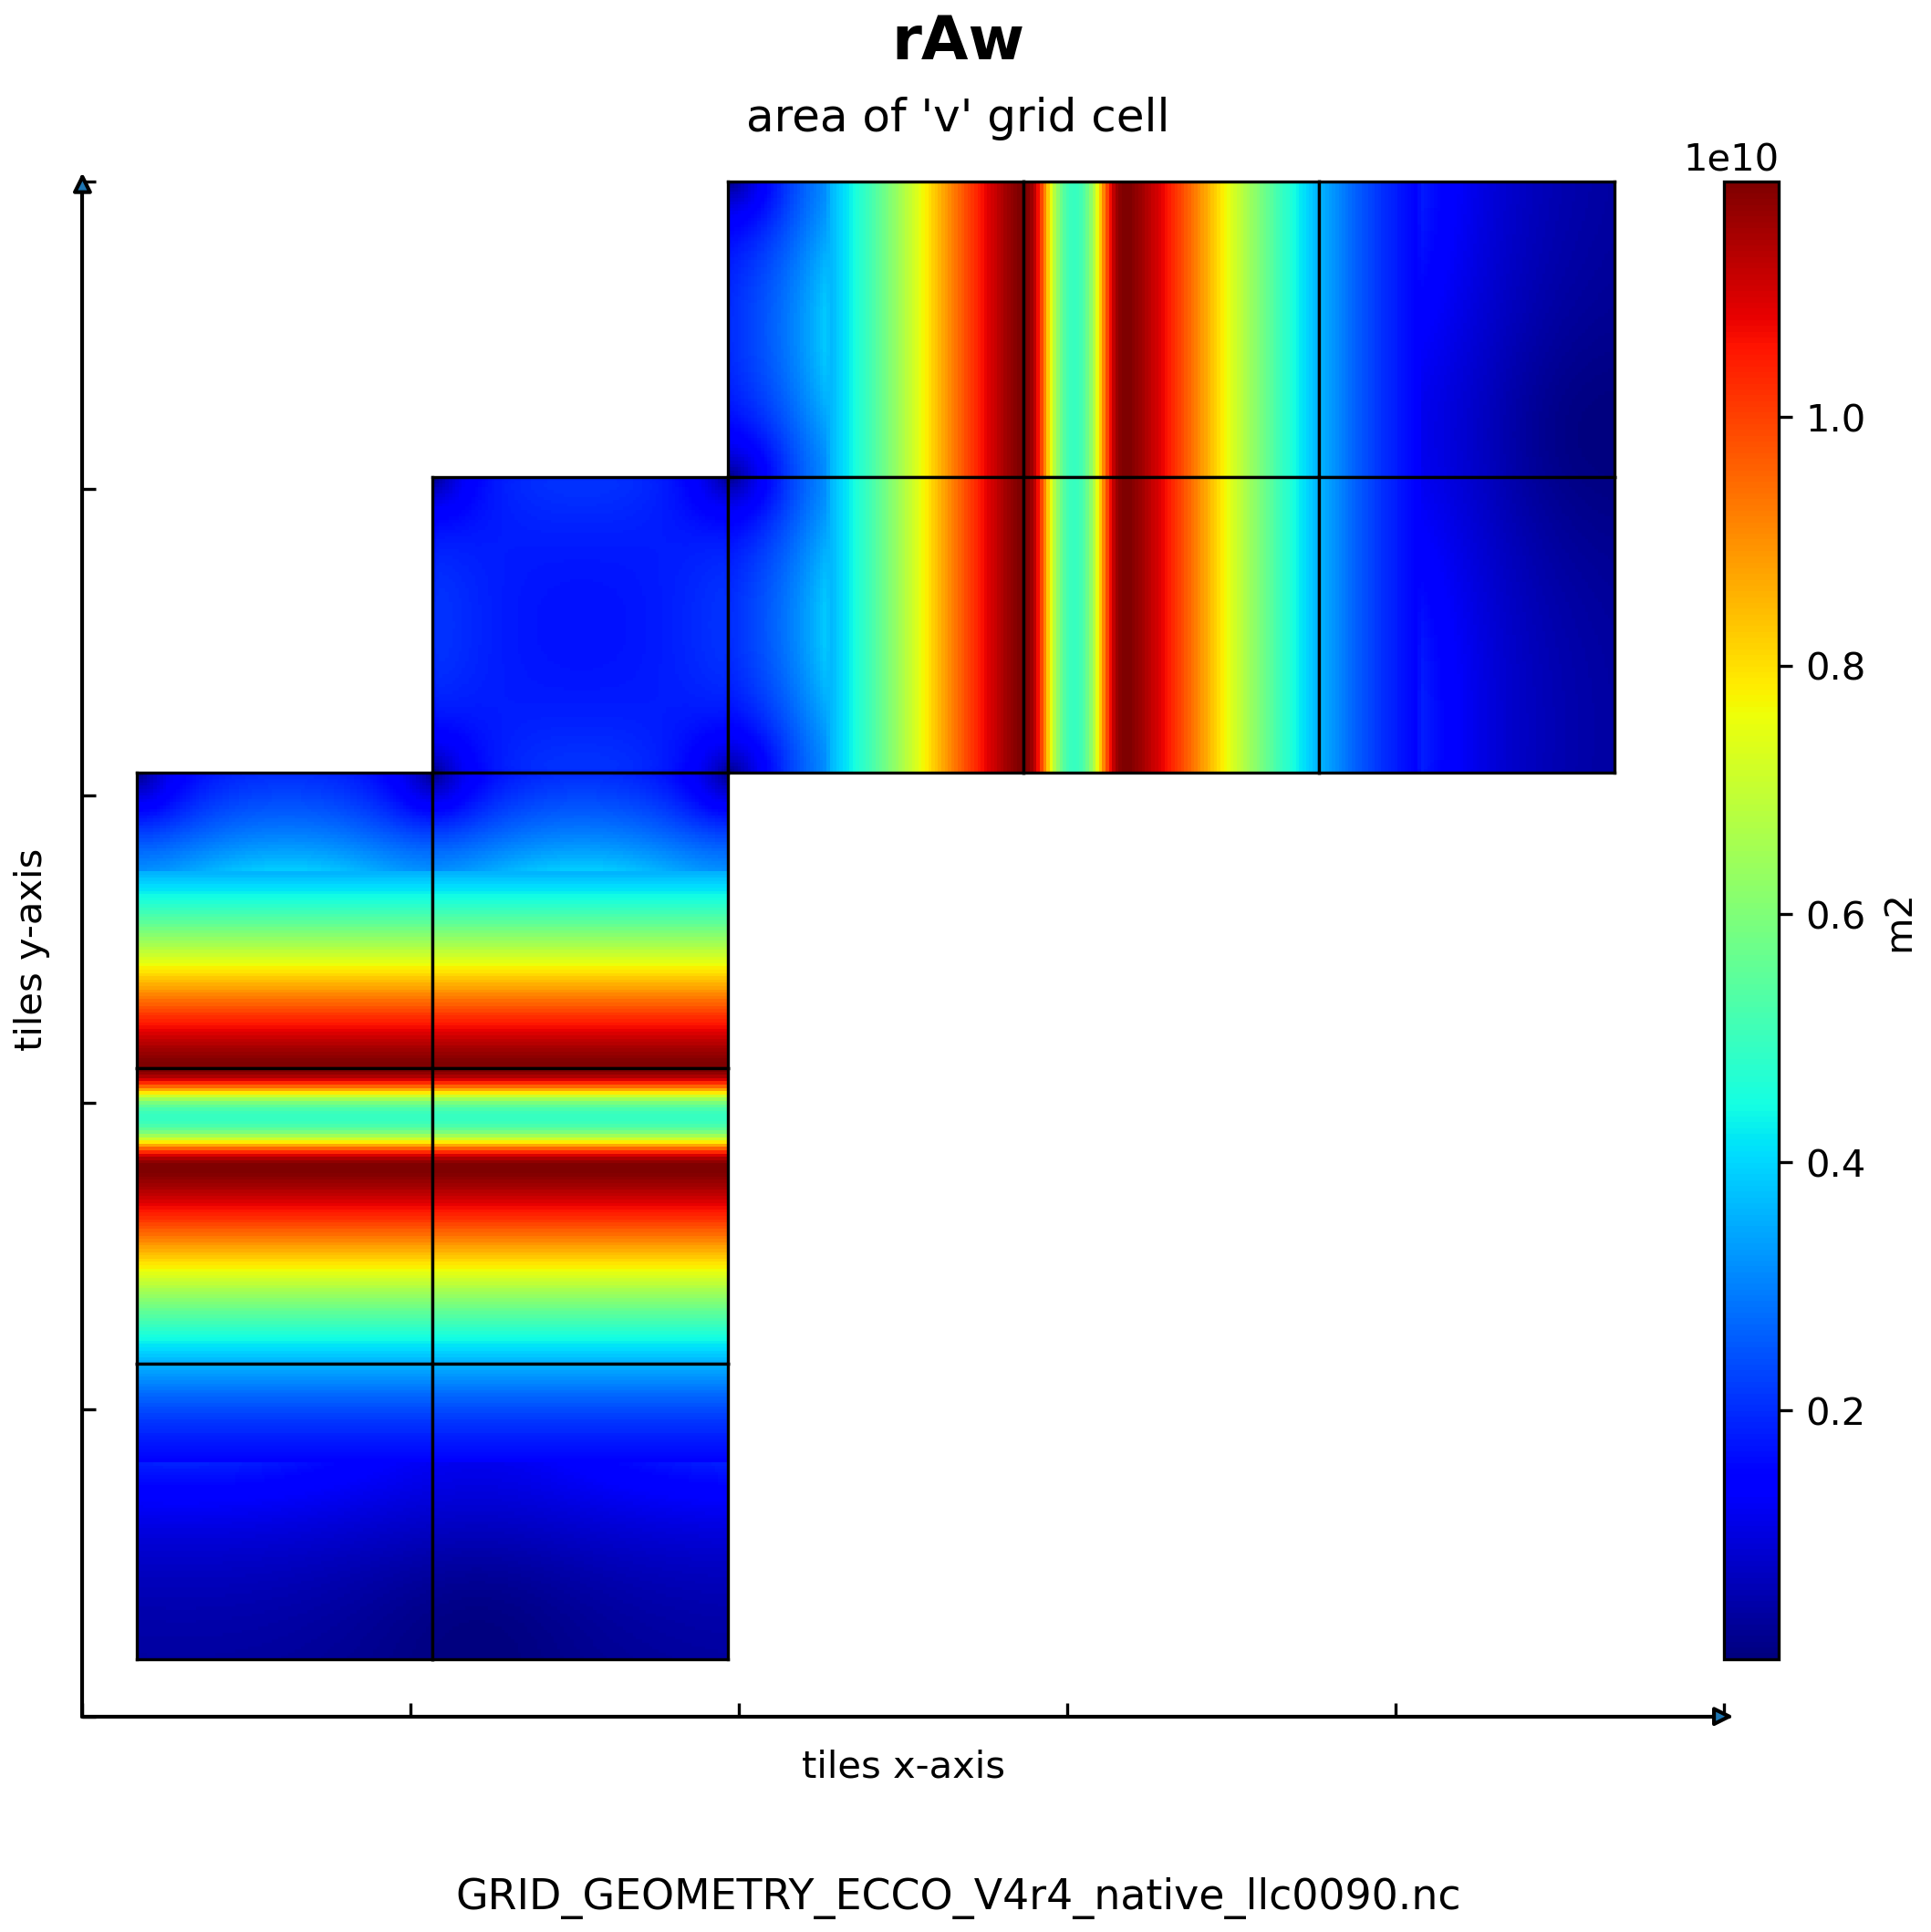
\includegraphics[scale=0.5]{../images/plots/native_plots_coords/Geometry_Parameters_for_the_Lat-Lon-Cap_90_(llc90)_Native_Model_Grid_(Version_4_Release_4)/rAw.png}
\caption{\\Dataset: GRID\_GEOMETRY\_ECCO\\Variable: rAw}
\label{tab:table-GRID_GEOMETRY_ECCO_rAw-Plot}
\end{figure}
\pagebreak
\subsubsection{Native coordinates Variable rAs}
\begin{longtable}{|p{0.06\textwidth}|p{0.41\textwidth}|p{0.39\textwidth}|p{0.06\textwidth}|}
    \caption{CDL description of GRID\_GEOMETRY\_ECCO's rAs variable}
    \label{tab:table-GRID_GEOMETRY_ECCO_rAs} \\ 
    \hline \endhead \hline \endfoot
    \rowcolor{lightgray} \textbf{Storage Type} & \textbf{Variable Name} & \textbf{Description} & \textbf{Unit} \\ \hline
    float32 & rAs & area of 'u' grid cell & m2 \\ \hline
    \rowcolor{lightgray}  \multicolumn{4}{|p{1.00\textwidth}|}{\textbf{CDL Description}} \\ \hline
    \multicolumn{4}{|p{1.00\textwidth}|}{\makecell{\parbox{1\textwidth}{float32 rAs(tile, j\_g, i)\\
    \hspace*{0.5cm}rAs: \_FillValue = 9.96921e+36\\
    \hspace*{0.5cm}rAs: long\_name = "area of u grid cell"\\
    \hspace*{0.5cm}rAs: units = m2\\
    \hspace*{0.5cm}rAs: coordinates = YG XC\\
    \hspace*{0.5cm}rAs: coverage\_content\_type = modelResult\\
    \hspace*{0.5cm}rAs: standard\_name = cell\_area}}} \\ \hline
    \rowcolor{lightgray} \multicolumn{4}{|p{1.00\textwidth}|}{\textbf{Comments}} \\ \hline
    \multicolumn{4}{|p{1\textwidth}|}{Model 'u' grid cells are staggered in space between adjacent tracer grid cells in the 'y' direction. 'u' grid cell (i,j) is situated at the 'south' edge of tracer grid cell (i, j). Note: 'south' does not correspond to geographic orientation but is used for convenience to describe the computational grid. See MITgcm documentation for details.} \\ \hline
\end{longtable}

\begin{figure}[H]
\centering
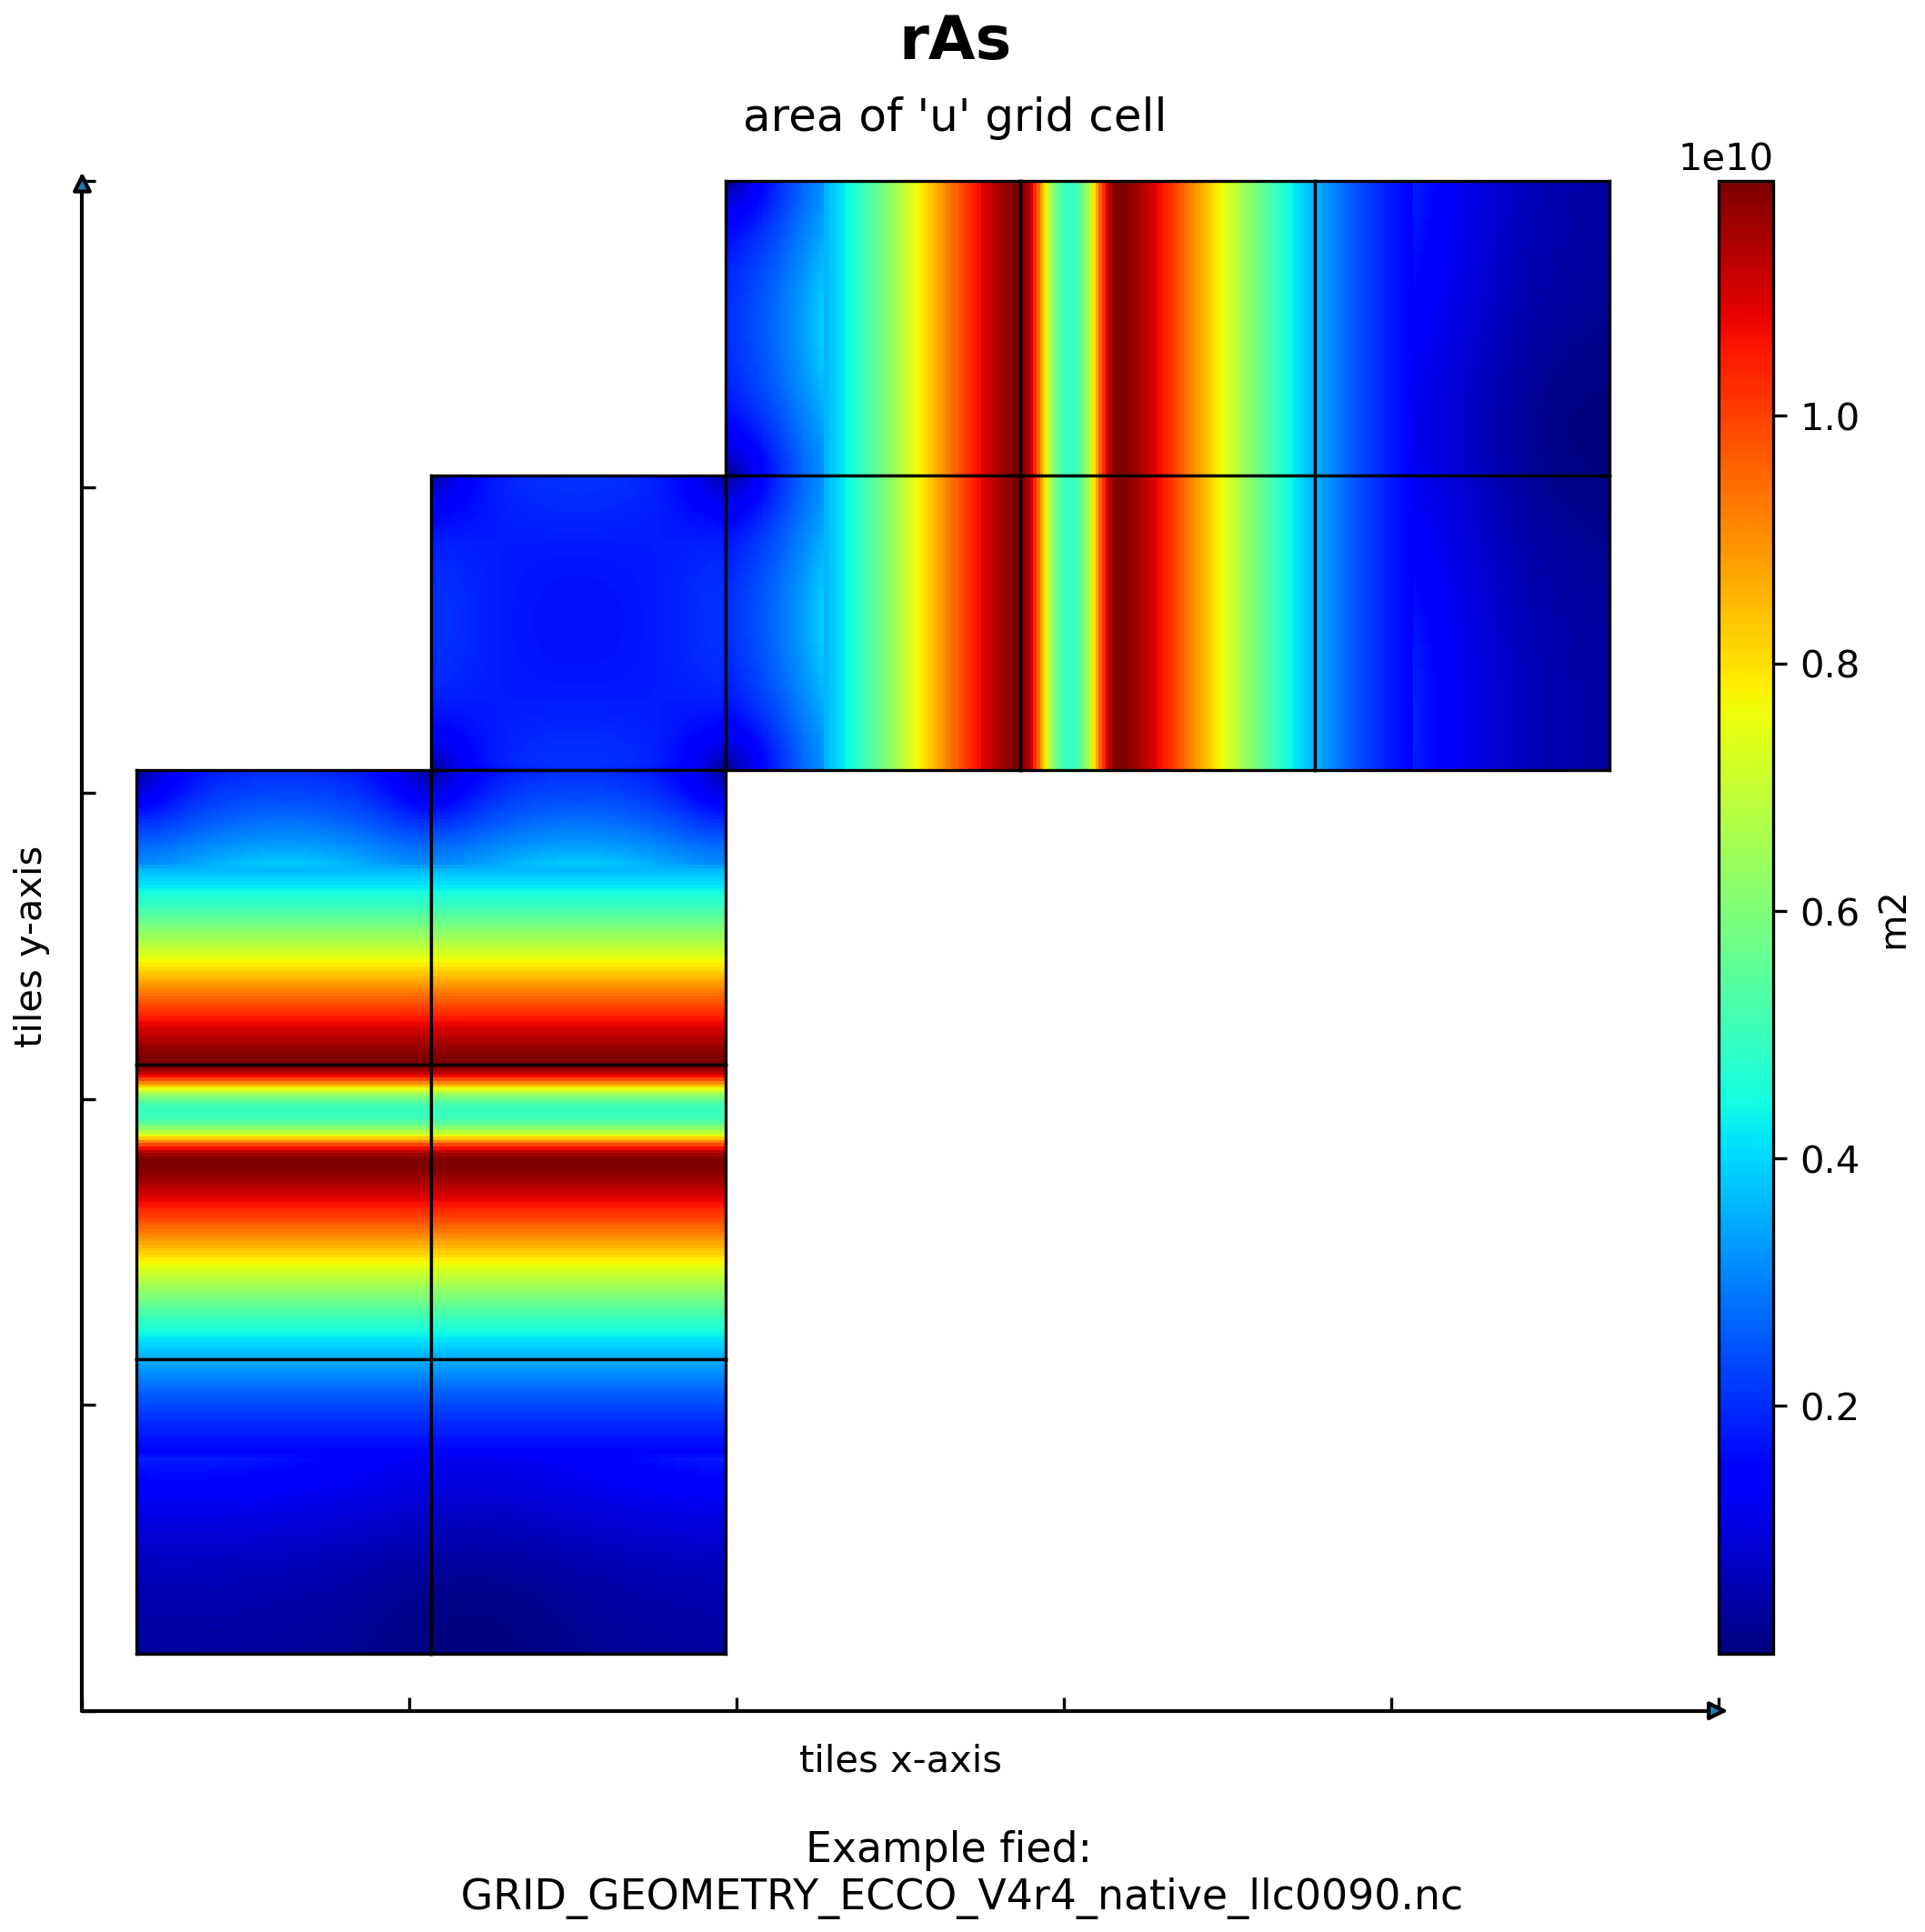
\includegraphics[scale=0.5]{../images/plots/native_plots_coords/Geometry_Parameters_for_the_Lat-Lon-Cap_90_(llc90)_Native_Model_Grid_(Version_4_Release_4)/rAs.png}
\caption{\\Dataset: GRID\_GEOMETRY\_ECCO\\Variable: rAs}
\label{tab:table-GRID_GEOMETRY_ECCO_rAs-Plot}
\end{figure}
\pagebreak
\subsubsection{Native coordinates Variable hFacC}
\begin{longtable}{|p{0.06\textwidth}|p{0.41\textwidth}|p{0.39\textwidth}|p{0.06\textwidth}|}
    \caption{CDL description of GRID\_GEOMETRY\_ECCO's hFacC variable}
    \label{tab:table-GRID_GEOMETRY_ECCO_hFacC} \\ 
    \hline \endhead \hline \endfoot
    \rowcolor{lightgray} \textbf{Storage Type} & \textbf{Variable Name} & \textbf{Description} & \textbf{Unit} \\ \hline
    float32 & hFacC & vertical open fraction of tracer grid cell & 1 \\ \hline
    \rowcolor{lightgray}  \multicolumn{4}{|p{1.00\textwidth}|}{\textbf{CDL Description}} \\ \hline
    \multicolumn{4}{|p{1.00\textwidth}|}{\makecell{\parbox{1\textwidth}{float32 hFacC(k, tile, j, i)\\
    \hspace*{0.5cm}hFacC: \_FillValue = 9.96921e+36\\
    \hspace*{0.5cm}hFacC: long\_name = vertical open fraction of tracer grid cell\\
    \hspace*{0.5cm}hFacC: coverage\_content\_type = modelResult\\
    \hspace*{0.5cm}hFacC: units = 1\\
    \hspace*{0.5cm}hFacC: coordinates = Z YC XC}}} \\ \hline
    \rowcolor{lightgray} \multicolumn{4}{|p{1.00\textwidth}|}{\textbf{Comments}} \\ \hline
    \multicolumn{4}{|p{1\textwidth}|}{Tracer grid cells may be fractionally closed in the vertical. The open vertical fraction is hFacC. The model allows for partially-filled cells to represent topographic variations more smoothly (hFacC < 1). Completely closed (dry) tracer grid cells have hFacC = 0. Note: the model z* coordinate system allows hFacC to vary through time. A time-invariant hFacC field is provided for reference.} \\ \hline
\end{longtable}

\begin{figure}[H]
\centering
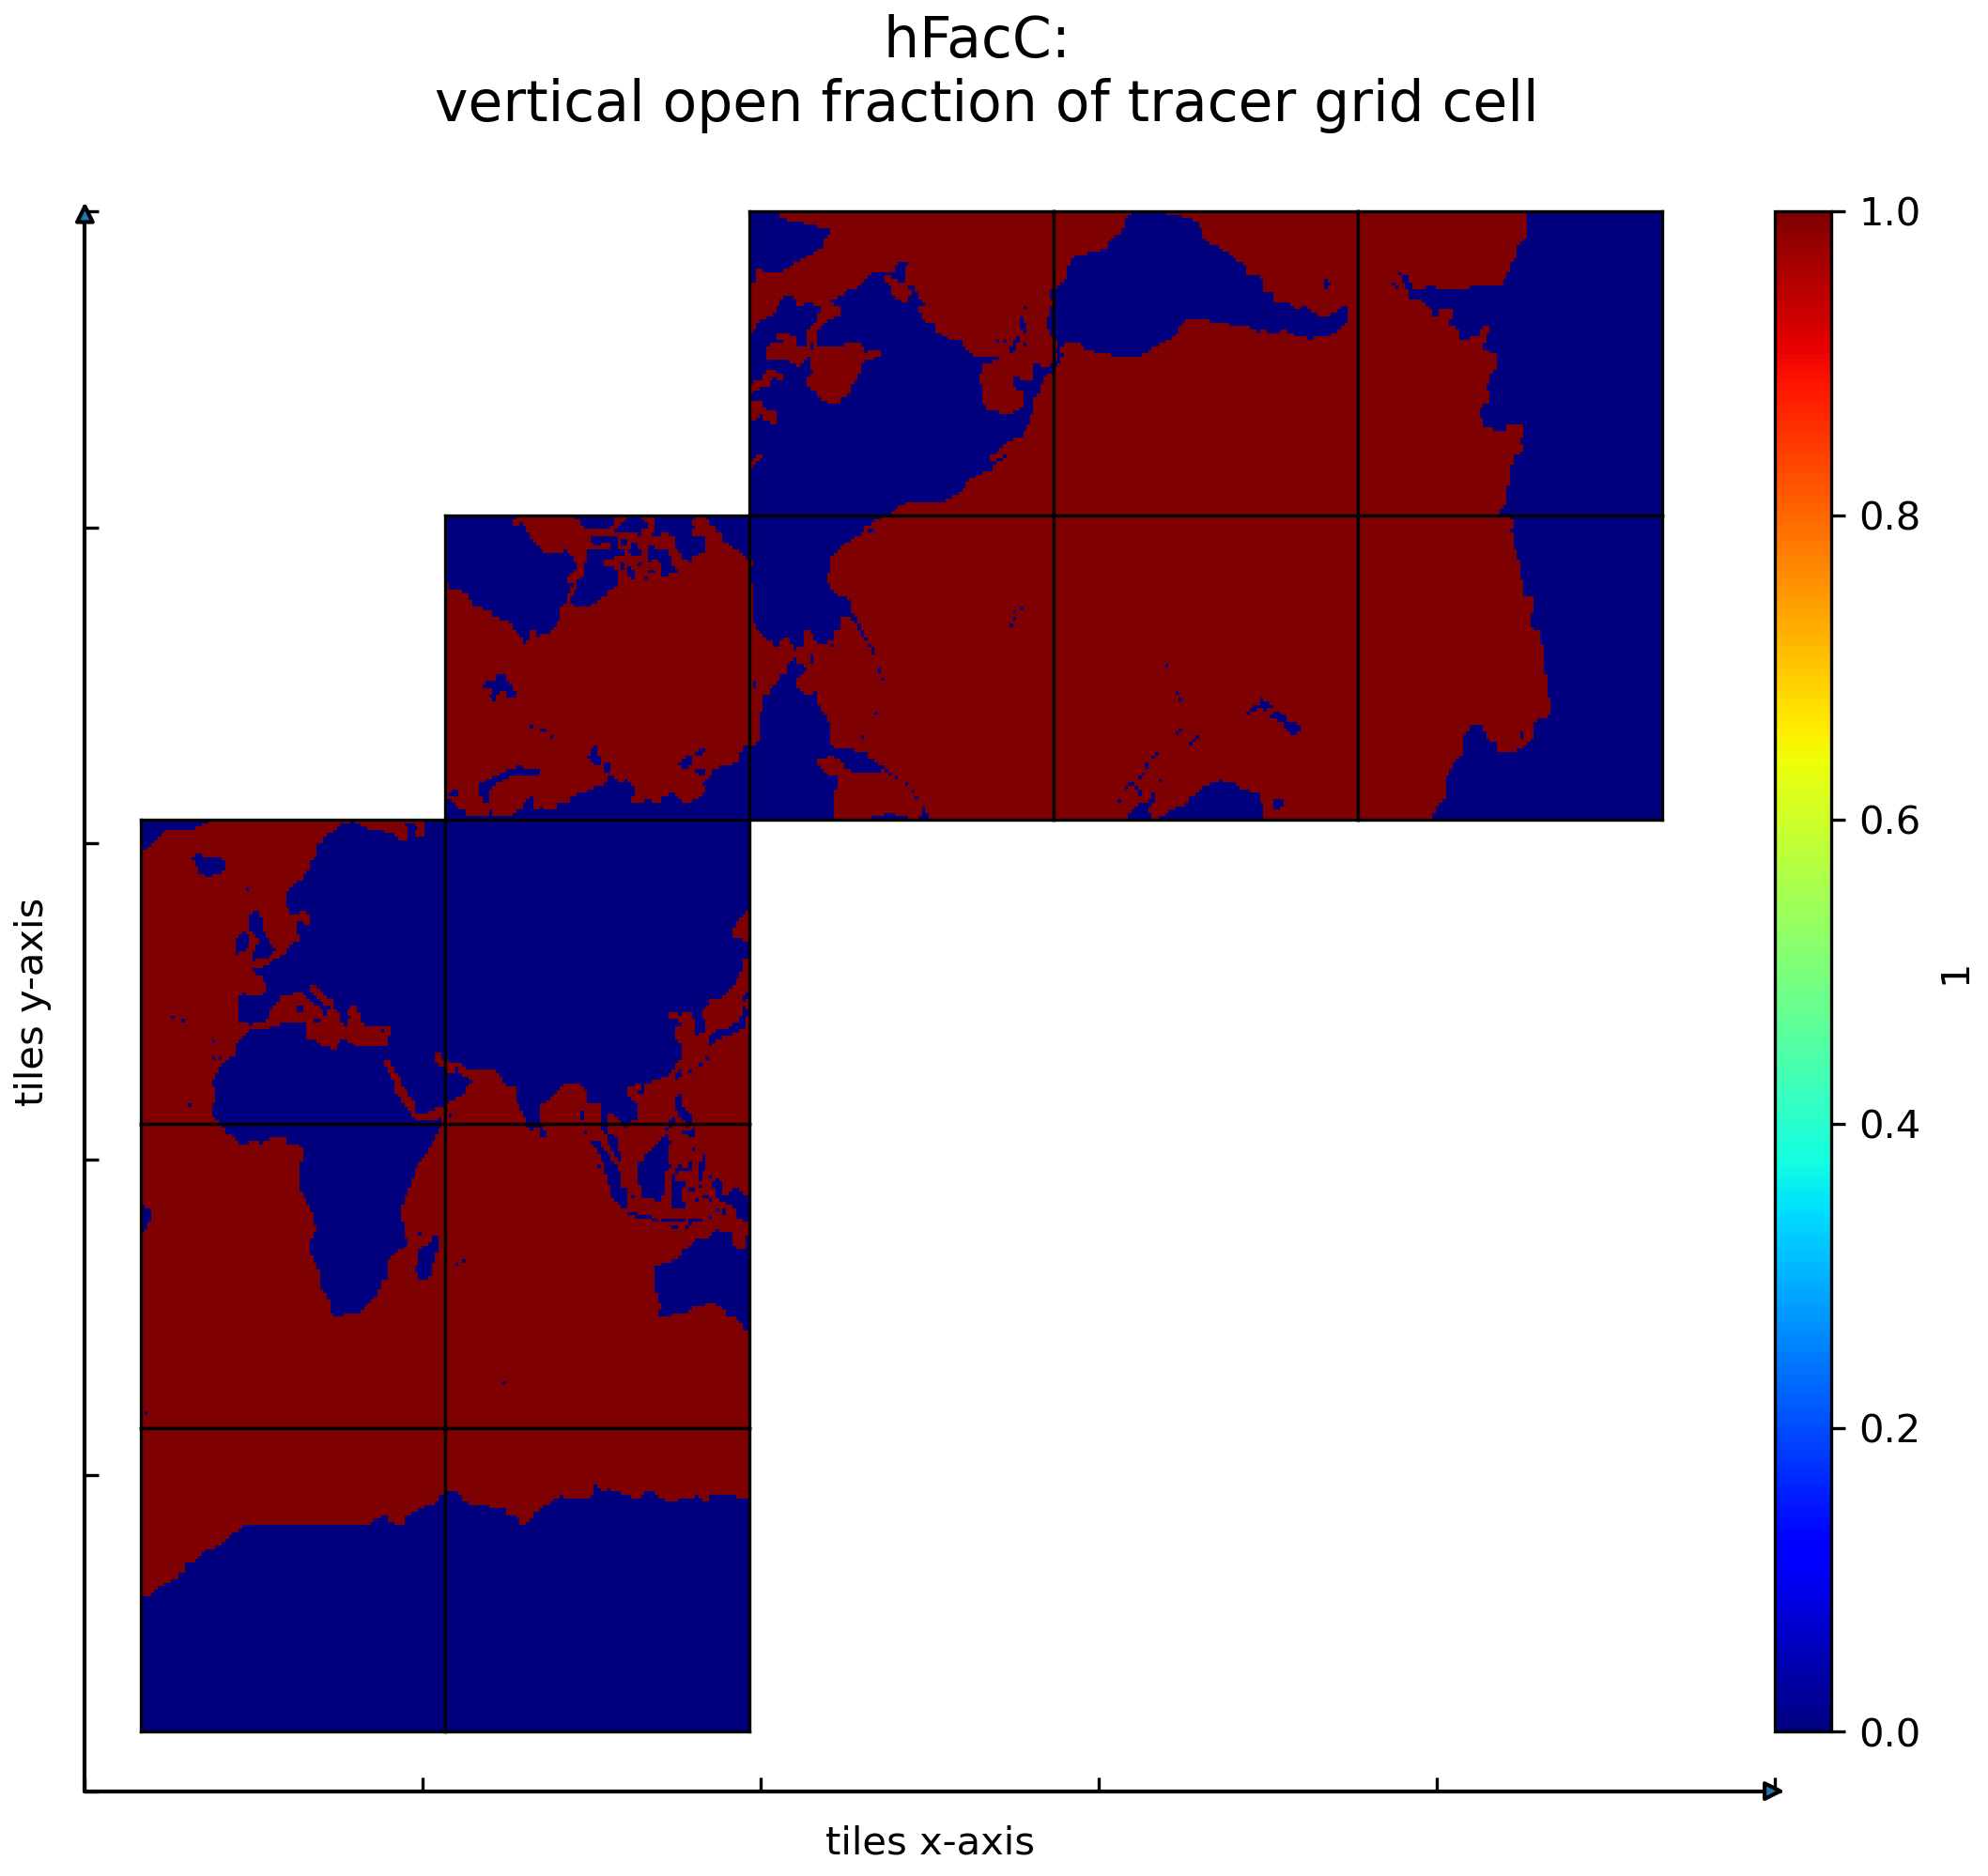
\includegraphics[scale=0.5]{../images/plots/native_plots_coords/Geometry_Parameters_for_the_Lat-Lon-Cap_90_(llc90)_Native_Model_Grid_(Version_4_Release_4)/hFacC.png}
\caption{\\Dataset: GRID\_GEOMETRY\_ECCO\\Variable: hFacC}
\label{tab:table-GRID_GEOMETRY_ECCO_hFacC-Plot}
\end{figure}
\pagebreak
\subsubsection{Native coordinates Variable hFacW}
\begin{longtable}{|p{0.06\textwidth}|p{0.41\textwidth}|p{0.39\textwidth}|p{0.06\textwidth}|}
    \caption{CDL description of GRID\_GEOMETRY\_ECCO's hFacW variable}
    \label{tab:table-GRID_GEOMETRY_ECCO_hFacW} \\ 
    \hline \endhead \hline \endfoot
    \rowcolor{lightgray} \textbf{Storage Type} & \textbf{Variable Name} & \textbf{Description} & \textbf{Unit} \\ \hline
    float32 & hFacW & vertical open fraction of tracer grid cell 'west' face & 1 \\ \hline
    \rowcolor{lightgray}  \multicolumn{4}{|p{1.00\textwidth}|}{\textbf{CDL Description}} \\ \hline
    \multicolumn{4}{|p{1.00\textwidth}|}{\makecell{\parbox{1\textwidth}{float32 hFacW(k, tile, j, i\_g)\\
    \hspace*{0.5cm}hFacW: \_FillValue = 9.96921e+36\\
    \hspace*{0.5cm}hFacW: long\_name = "vertical open fraction of tracer grid cell west face"\\
    \hspace*{0.5cm}hFacW: coverage\_content\_type = modelResult\\
    \hspace*{0.5cm}hFacW: units = 1\\
    \hspace*{0.5cm}hFacW: coordinates = Z}}} \\ \hline
    \rowcolor{lightgray} \multicolumn{4}{|p{1.00\textwidth}|}{\textbf{Comments}} \\ \hline
    \multicolumn{4}{|p{1\textwidth}|}{The 'west' face of tracer grid cells may be fractionally closed in the vertical. The open vertical fraction is hFacW. The model allows for partially-filled cells for smoother representation of seafloor topography. Tracer grid cells adjacent in the 'x' direction that are partially closed in the vertical have hFacW < 1. The model z* coordinate system used by the model permits hFacC, and therefore hFacW, to vary through time. A time-invariant hFacW field is provided for reference. Note: The term 'west' does not correspond to geographic orientation but is used for convenience to describe the computational grid. See MITgcm documentation for details.} \\ \hline
\end{longtable}

\begin{figure}[H]
\centering
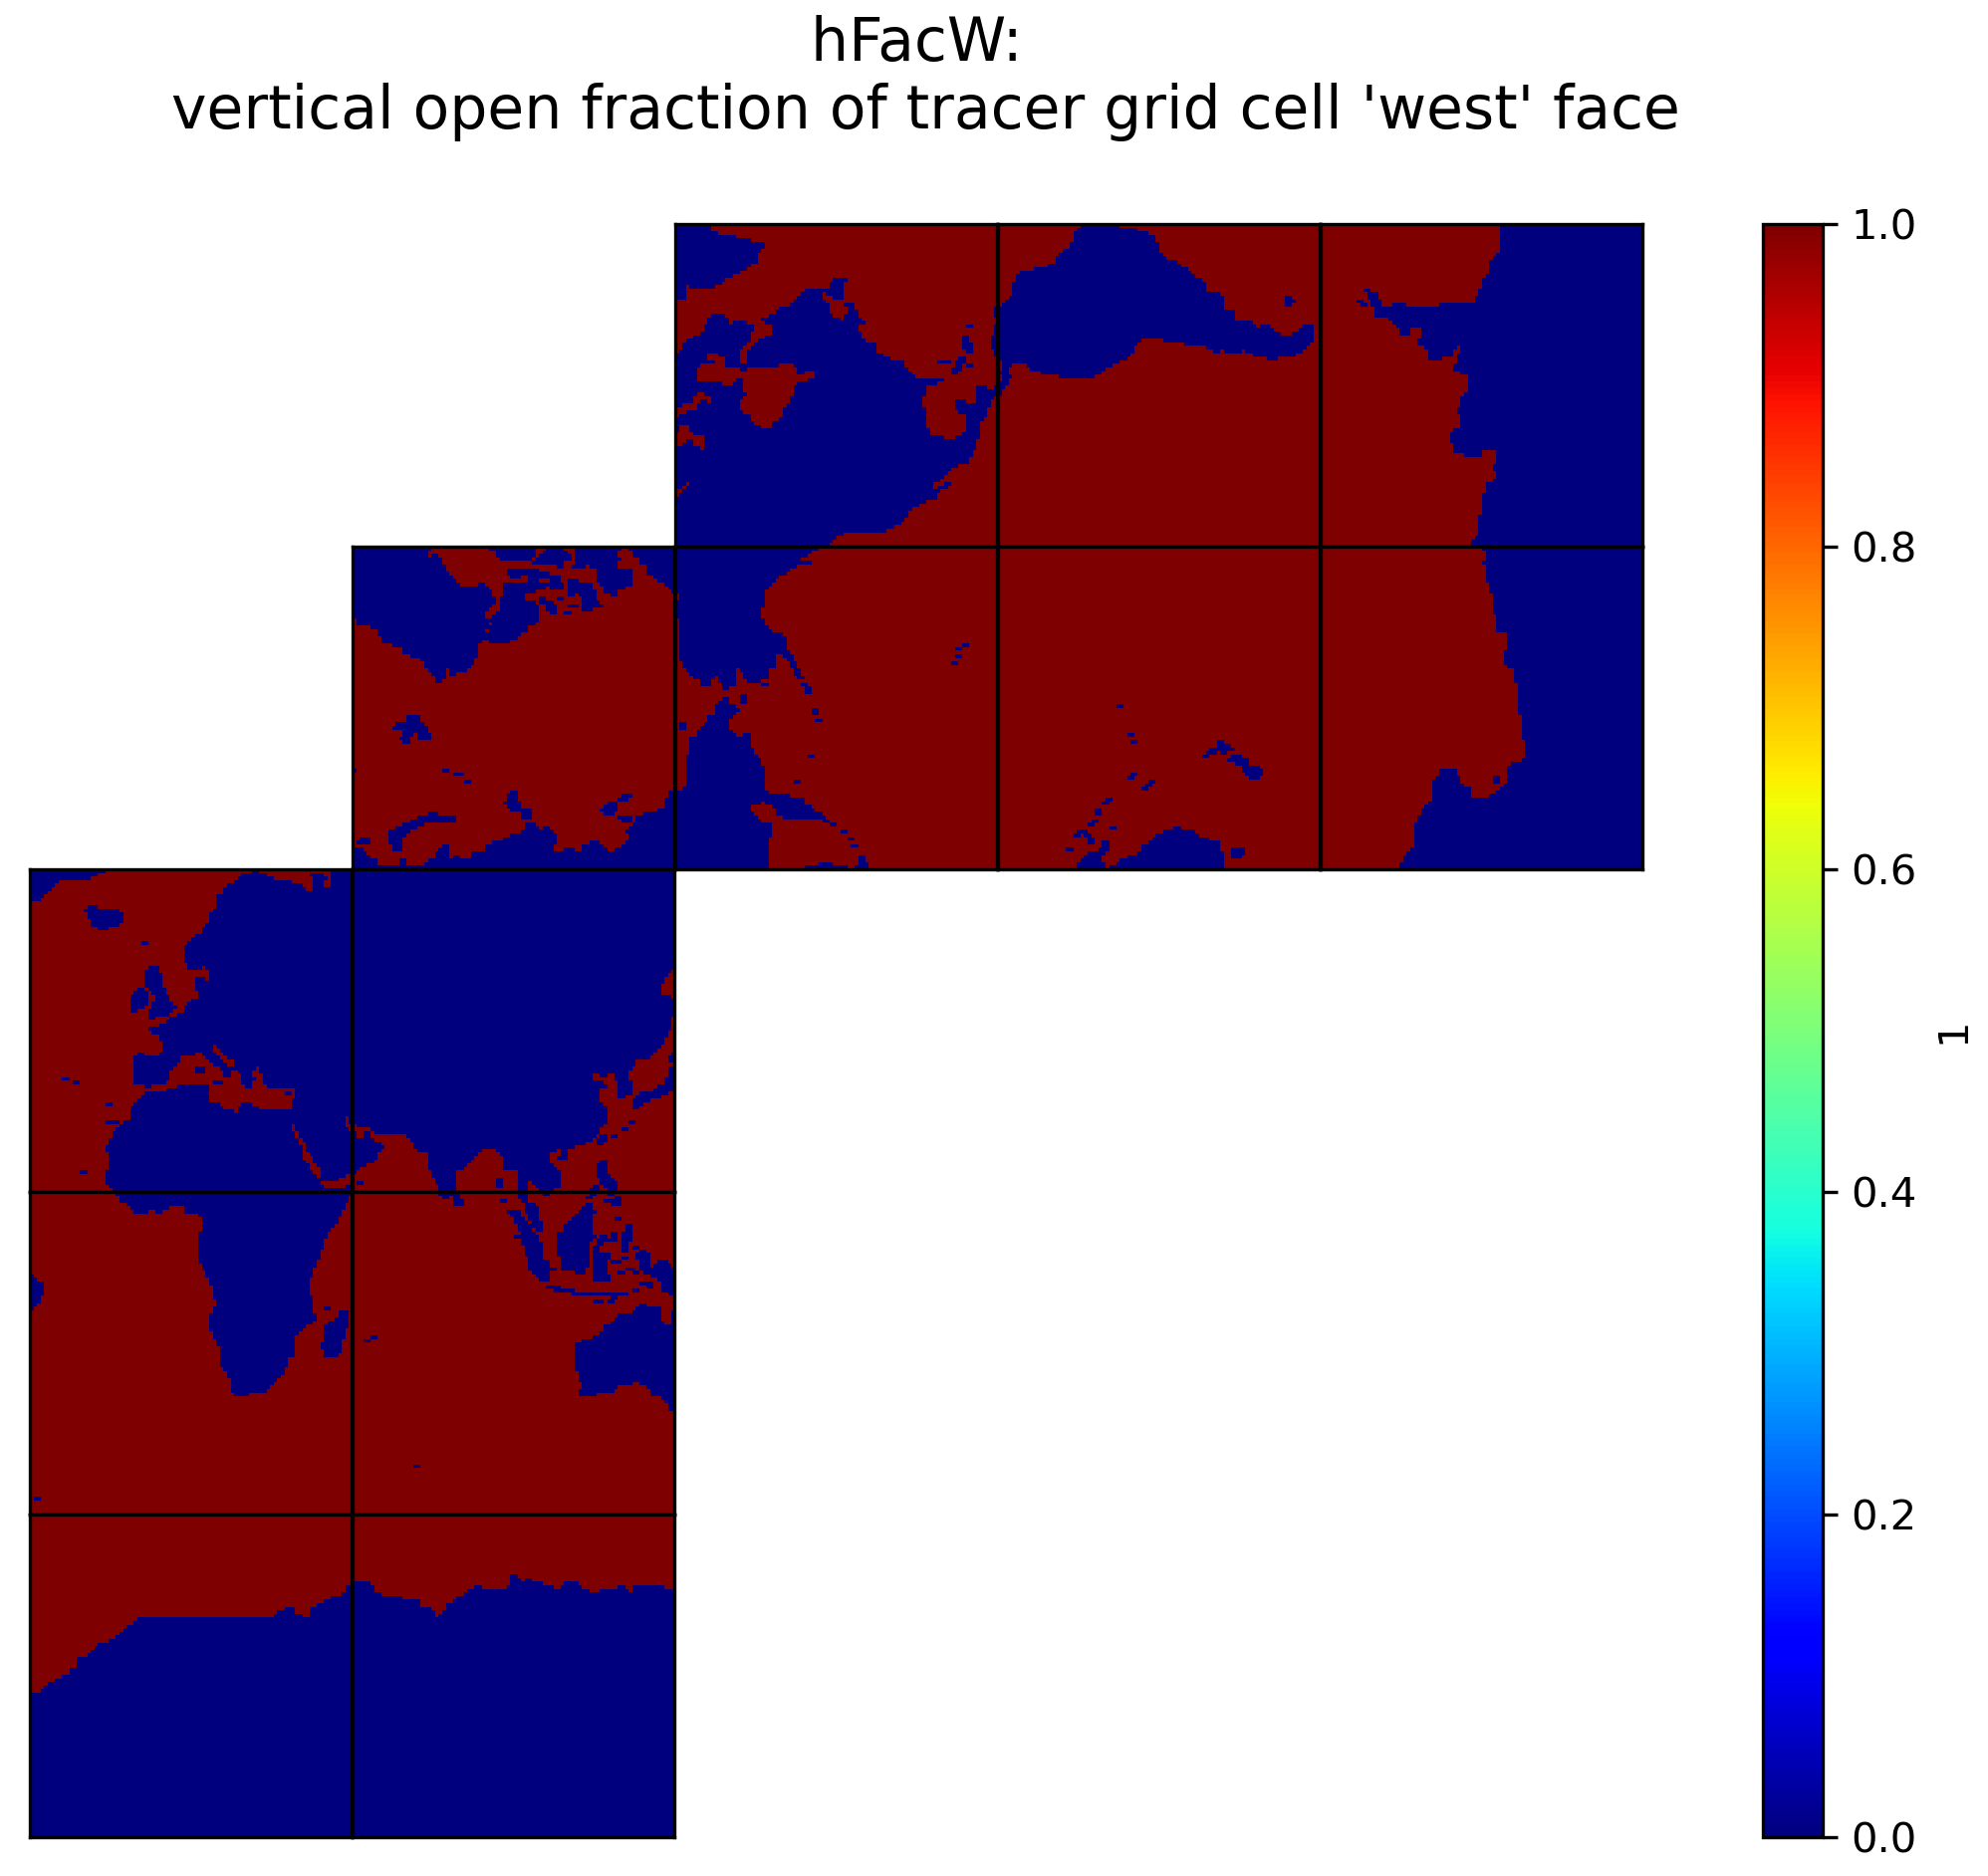
\includegraphics[scale=0.5]{../images/plots/native_plots_coords/Geometry_Parameters_for_the_Lat-Lon-Cap_90_(llc90)_Native_Model_Grid_(Version_4_Release_4)/hFacW.png}
\caption{\\Dataset: GRID\_GEOMETRY\_ECCO\\Variable: hFacW}
\label{tab:table-GRID_GEOMETRY_ECCO_hFacW-Plot}
\end{figure}
\pagebreak
\subsubsection{Native coordinates Variable hFacS}
\begin{longtable}{|p{0.06\textwidth}|p{0.41\textwidth}|p{0.39\textwidth}|p{0.06\textwidth}|}
    \caption{CDL description of GRID\_GEOMETRY\_ECCO's hFacS variable}
    \label{tab:table-GRID_GEOMETRY_ECCO_hFacS} \\ 
    \hline \endhead \hline \endfoot
    \rowcolor{lightgray} \textbf{Storage Type} & \textbf{Variable Name} & \textbf{Description} & \textbf{Unit} \\ \hline
    float32 & hFacS & vertical open fraction of tracer grid cell 'south' face & 1 \\ \hline
    \rowcolor{lightgray}  \multicolumn{4}{|p{1.00\textwidth}|}{\textbf{CDL Description}} \\ \hline
    \multicolumn{4}{|p{1.00\textwidth}|}{\makecell{\parbox{1\textwidth}{float32 hFacS(k, tile, j\_g, i)\\
    \hspace*{0.5cm}hFacS: \_FillValue = 9.96921e+36\\
    \hspace*{0.5cm}hFacS: long\_name = "vertical open fraction of tracer grid cell south face"\\
    \hspace*{0.5cm}hFacS: coverage\_content\_type = modelResult\\
    \hspace*{0.5cm}hFacS: units = 1\\
    \hspace*{0.5cm}hFacS: coordinates = Z}}} \\ \hline
    \rowcolor{lightgray} \multicolumn{4}{|p{1.00\textwidth}|}{\textbf{Comments}} \\ \hline
    \multicolumn{4}{|p{1\textwidth}|}{The 'south' face of tracer grid cells may be fractionally closed in the vertical. The open vertical fraction is hFacS. The model allows for partially-filled cells for smoother representation of seafloor topography. Tracer grid cells adjacent in the 'y' direction that are partially closed in the vertical have hFacS < 1. The model z* coordinate system used by the model permits hFacC, and therefore hFacS, to vary through time. A time-invariant hFacS field is provided for reference. Note:  The term 'south' does not correspond to geographic orientation but is used for convenience to describe the computational grid. See MITgcm documentation for details.} \\ \hline
\end{longtable}

\begin{figure}[H]
\centering
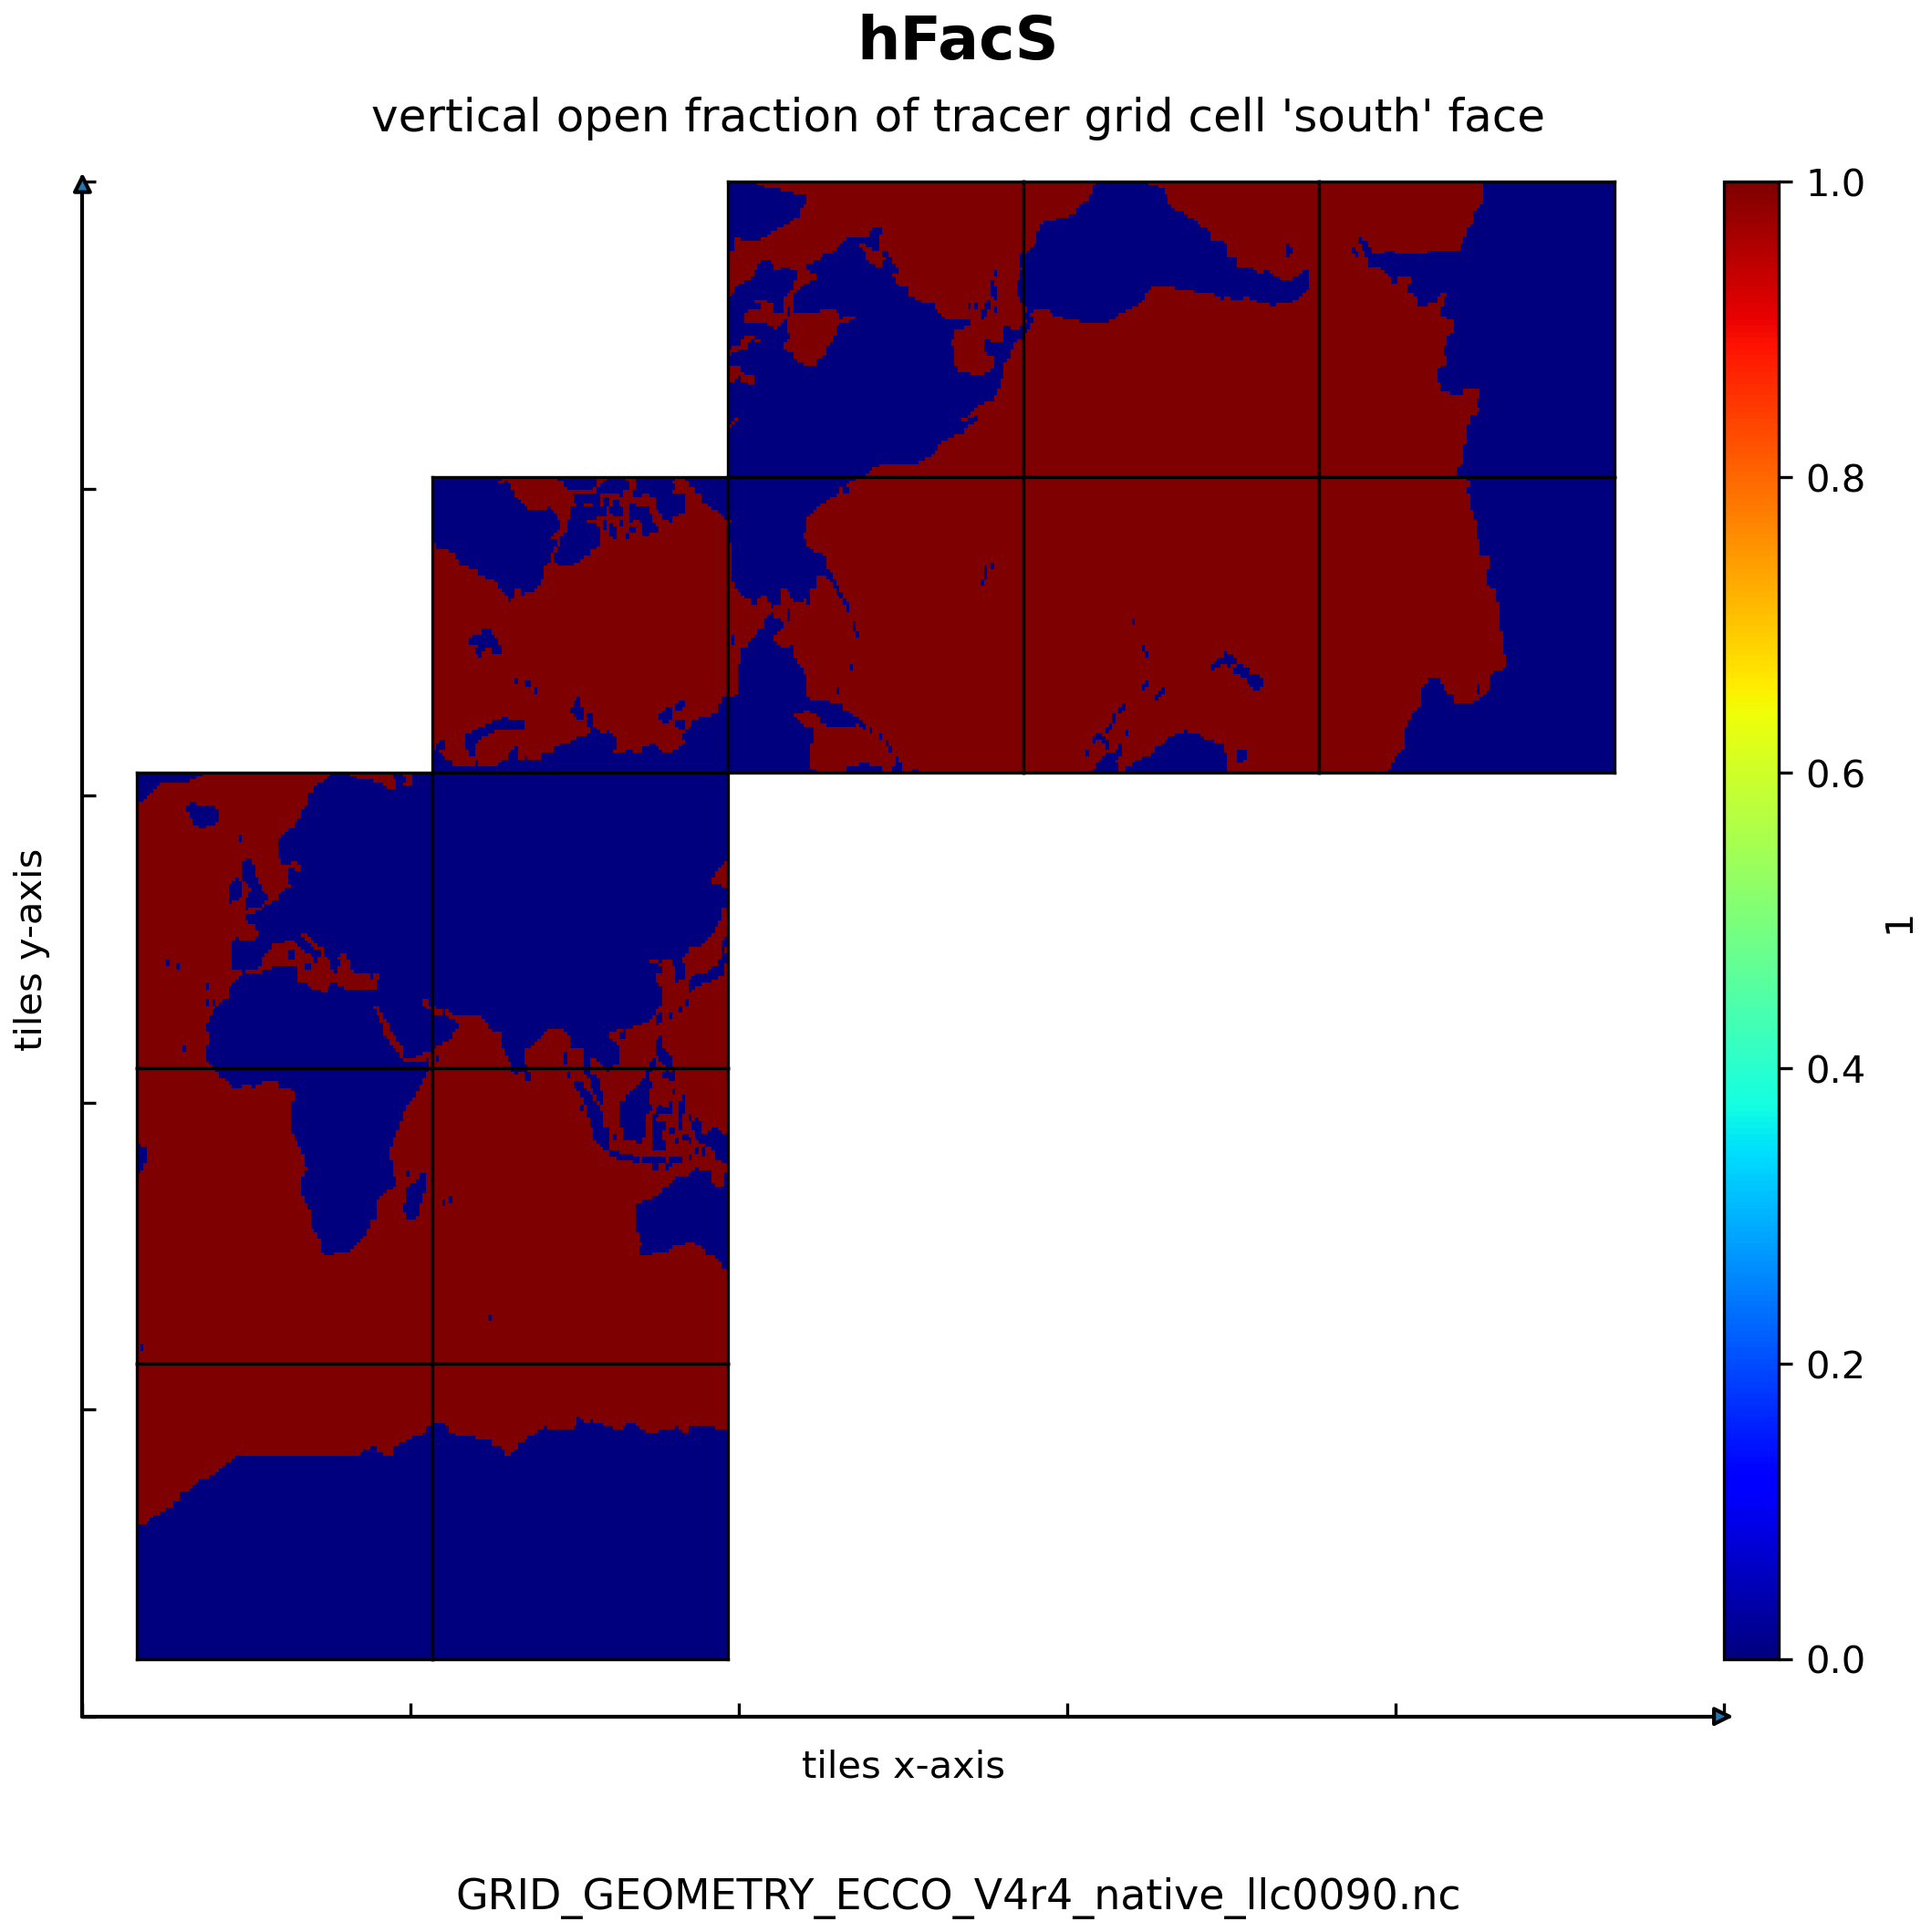
\includegraphics[scale=0.5]{../images/plots/native_plots_coords/Geometry_Parameters_for_the_Lat-Lon-Cap_90_(llc90)_Native_Model_Grid_(Version_4_Release_4)/hFacS.png}
\caption{\\Dataset: GRID\_GEOMETRY\_ECCO\\Variable: hFacS}
\label{tab:table-GRID_GEOMETRY_ECCO_hFacS-Plot}
\end{figure}
\pagebreak
\subsubsection{Native coordinates Variable maskC}
\begin{longtable}{|p{0.06\textwidth}|p{0.41\textwidth}|p{0.39\textwidth}|p{0.06\textwidth}|}
    \caption{CDL description of GRID\_GEOMETRY\_ECCO's maskC variable}
    \label{tab:table-GRID_GEOMETRY_ECCO_maskC} \\ 
    \hline \endhead \hline \endfoot
    \rowcolor{lightgray} \textbf{Storage Type} & \textbf{Variable Name} & \textbf{Description} & \textbf{Unit} \\ \hline
    bool & maskC & wet/dry boolean mask for tracer grid cell & N/A \\ \hline
    \rowcolor{lightgray}  \multicolumn{4}{|p{1.00\textwidth}|}{\textbf{CDL Description}} \\ \hline
    \multicolumn{4}{|p{1.00\textwidth}|}{\makecell{\parbox{1\textwidth}{bool maskC(k, tile, j, i)\\
    \hspace*{0.5cm}maskC: \_FillValue = 1\\
    \hspace*{0.5cm}maskC: long\_name = wet/dry boolean mask for tracer grid cell\\
    \hspace*{0.5cm}maskC: coverage\_content\_type = modelResult\\
    \hspace*{0.5cm}maskC: coordinates = Z YC XC}}} \\ \hline
    \rowcolor{lightgray} \multicolumn{4}{|p{1.00\textwidth}|}{\textbf{Comments}} \\ \hline
    \multicolumn{4}{|p{1\textwidth}|}{True for tracer grid cells with nonzero open vertical fraction (hFacC > 0), otherwise False. Although hFacC can vary though time, cells will never close if starting open and will never open if starting closed: hFacC(i,j,k,t) > 0 for all t, if hFacC(i,j,k,t=0) and hFacC(i,j,k,t) = 0 for all t, if hFacC(i,j,k,t=0) = 0. Therefore, maskC is time invariant.} \\ \hline
\end{longtable}

\begin{figure}[H]
\centering
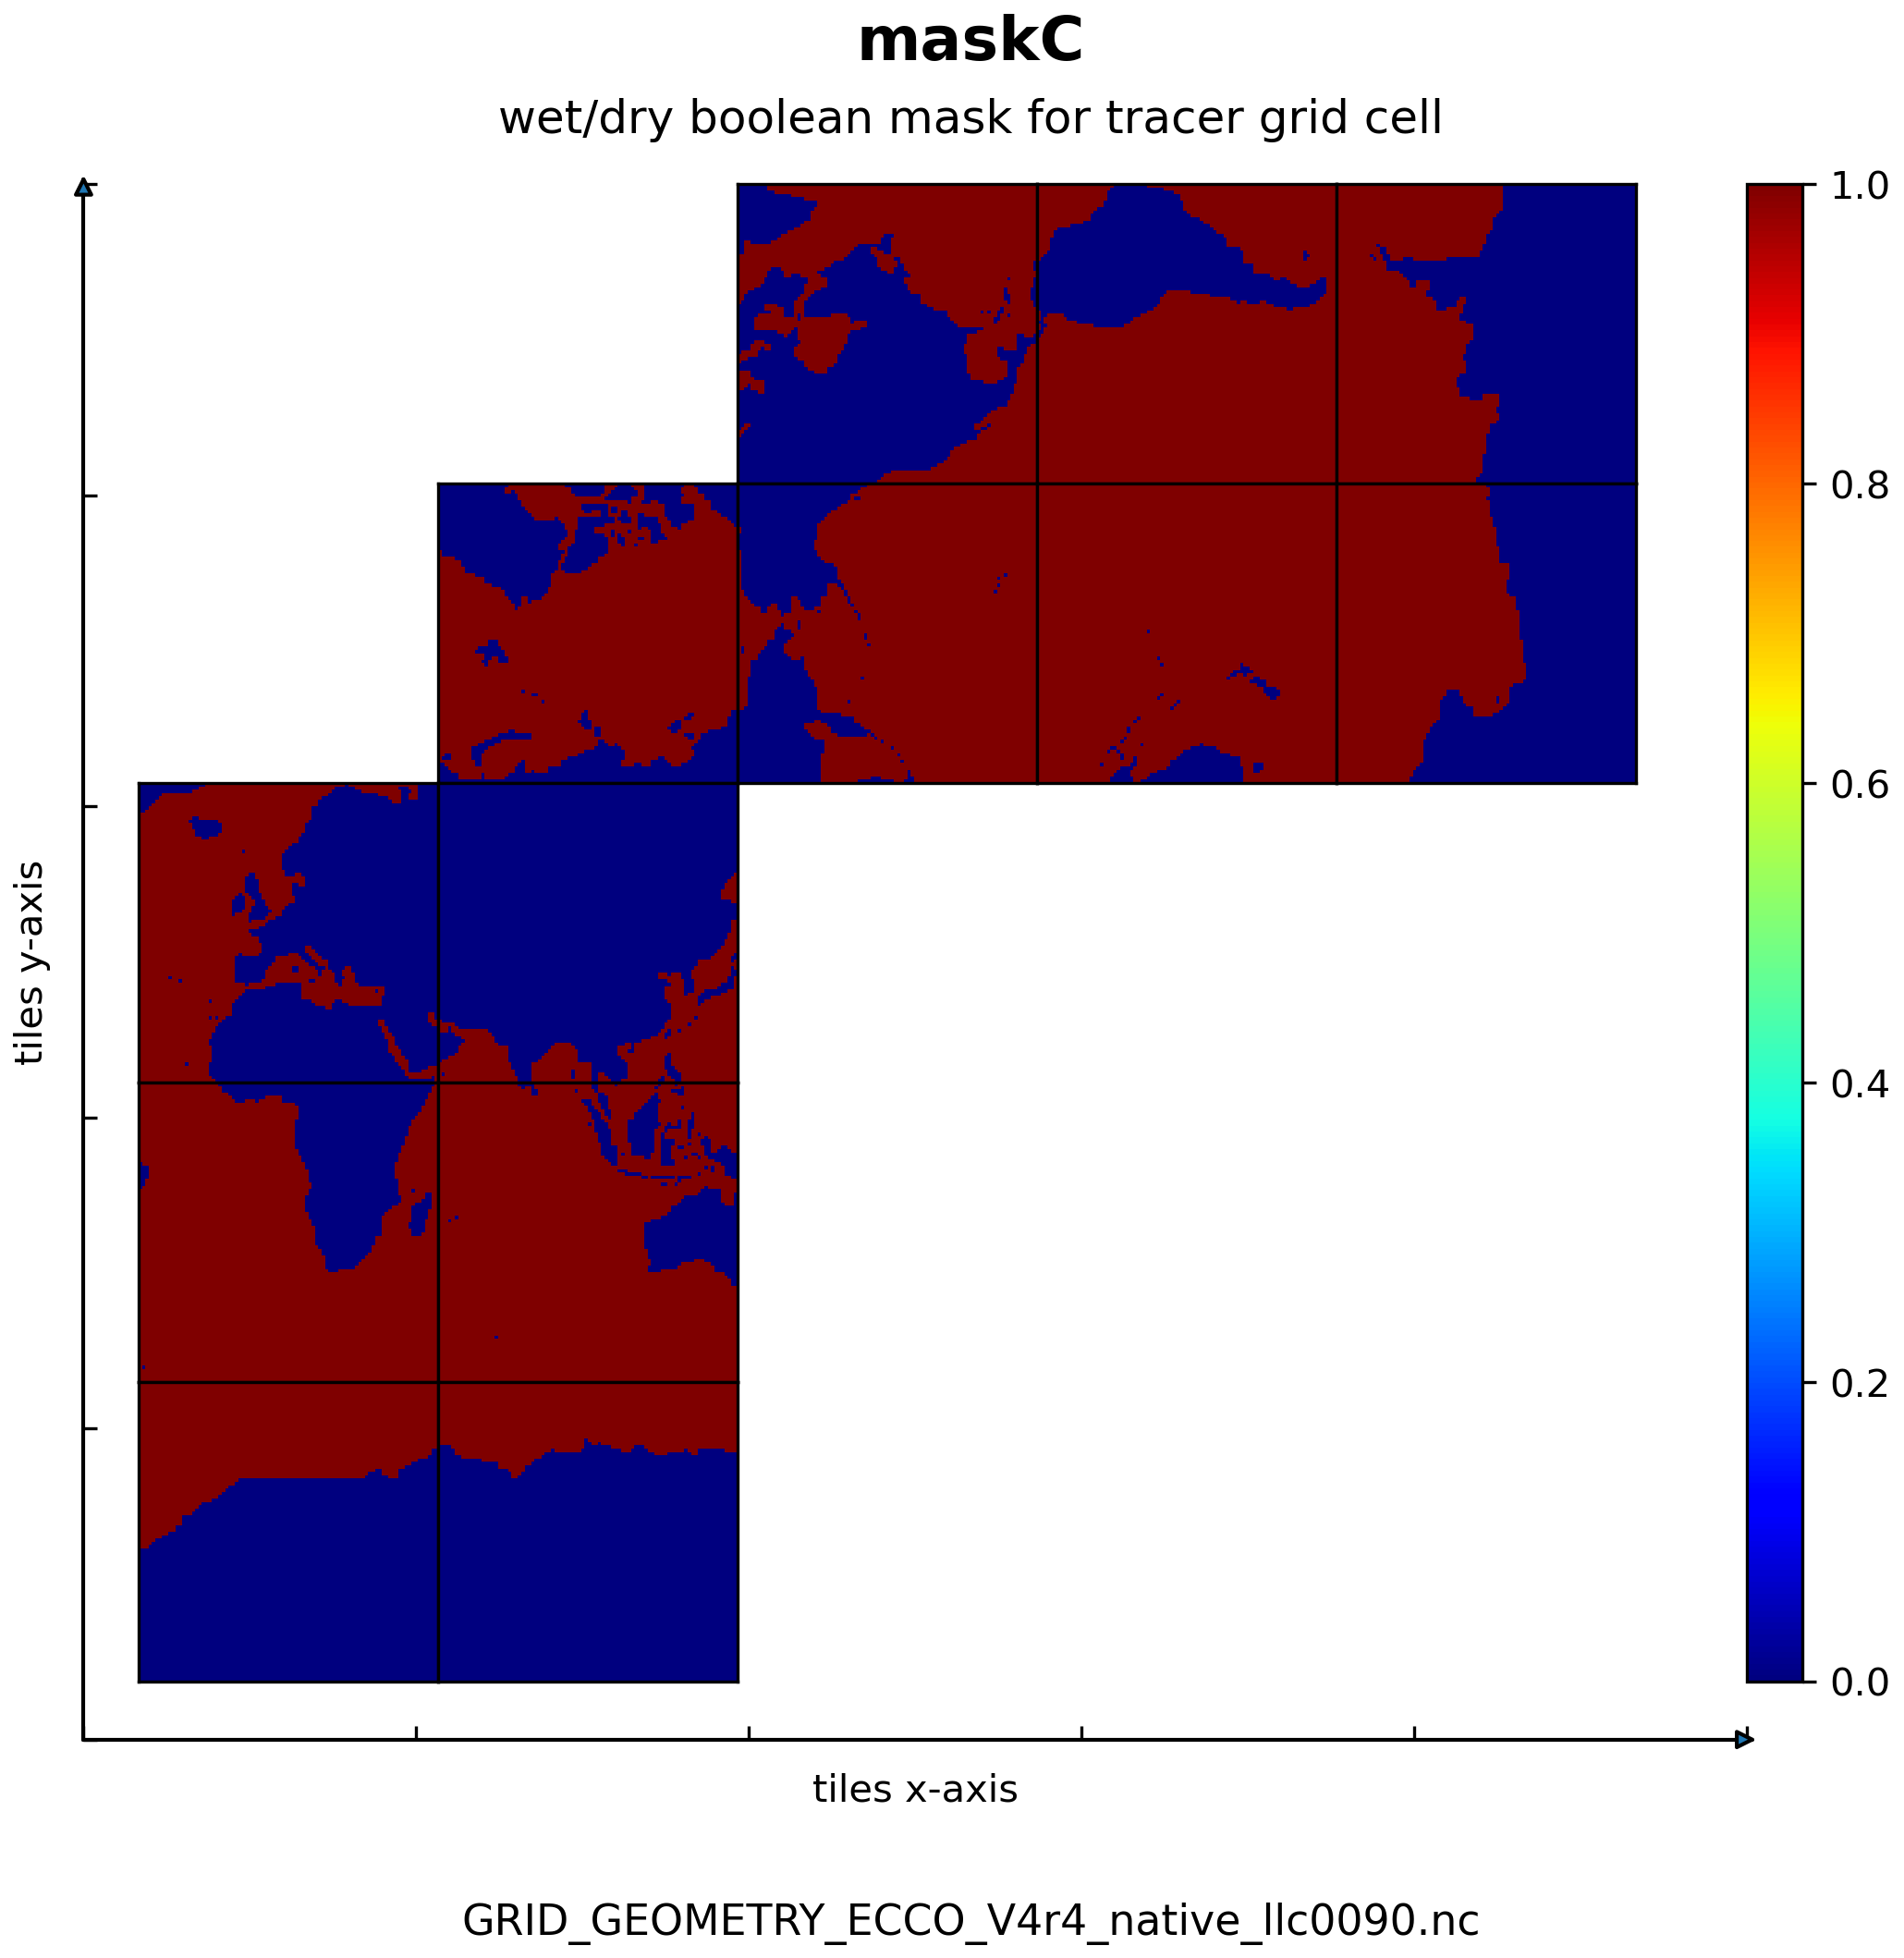
\includegraphics[scale=0.5]{../images/plots/native_plots_coords/Geometry_Parameters_for_the_Lat-Lon-Cap_90_(llc90)_Native_Model_Grid_(Version_4_Release_4)/maskC.png}
\caption{\\Dataset: GRID\_GEOMETRY\_ECCO\\Variable: maskC}
\label{tab:table-GRID_GEOMETRY_ECCO_maskC-Plot}
\end{figure}
\pagebreak
\subsubsection{Native coordinates Variable maskW}
\begin{longtable}{|p{0.06\textwidth}|p{0.41\textwidth}|p{0.39\textwidth}|p{0.06\textwidth}|}
    \caption{CDL description of GRID\_GEOMETRY\_ECCO's maskW variable}
    \label{tab:table-GRID_GEOMETRY_ECCO_maskW} \\ 
    \hline \endhead \hline \endfoot
    \rowcolor{lightgray} \textbf{Storage Type} & \textbf{Variable Name} & \textbf{Description} & \textbf{Unit} \\ \hline
    bool & maskW & wet/dry boolean mask for 'west' face of tracer grid cell & N/A \\ \hline
    \rowcolor{lightgray}  \multicolumn{4}{|p{1.00\textwidth}|}{\textbf{CDL Description}} \\ \hline
    \multicolumn{4}{|p{1.00\textwidth}|}{\makecell{\parbox{1\textwidth}{bool maskW(k, tile, j, i\_g)\\
    \hspace*{0.5cm}maskW: \_FillValue = 1\\
    \hspace*{0.5cm}maskW: long\_name = "wet/dry boolean mask for west face of tracer grid cell"\\
    \hspace*{0.5cm}maskW: coverage\_content\_type = modelResult\\
    \hspace*{0.5cm}maskW: coordinates = Z}}} \\ \hline
    \rowcolor{lightgray} \multicolumn{4}{|p{1.00\textwidth}|}{\textbf{Comments}} \\ \hline
    \multicolumn{4}{|p{1\textwidth}|}{True for grid cells with nonzero open vertical fraction along their 'west' face (hFacW > 0), otherwise False. Although hFacW can vary though time, cells will never close if starting open and will never open if starting closed: hFacW(i,j,k,t) > 0 for all t, if hFacW(i,j,k,t=0) and hFacW(i,j,k,t) = 0 for all t, if hFacW(i,j,k,t=0) = 0. Therefore, maskW is time invariant. Note: } \\ \hline
\end{longtable}

\begin{figure}[H]
\centering
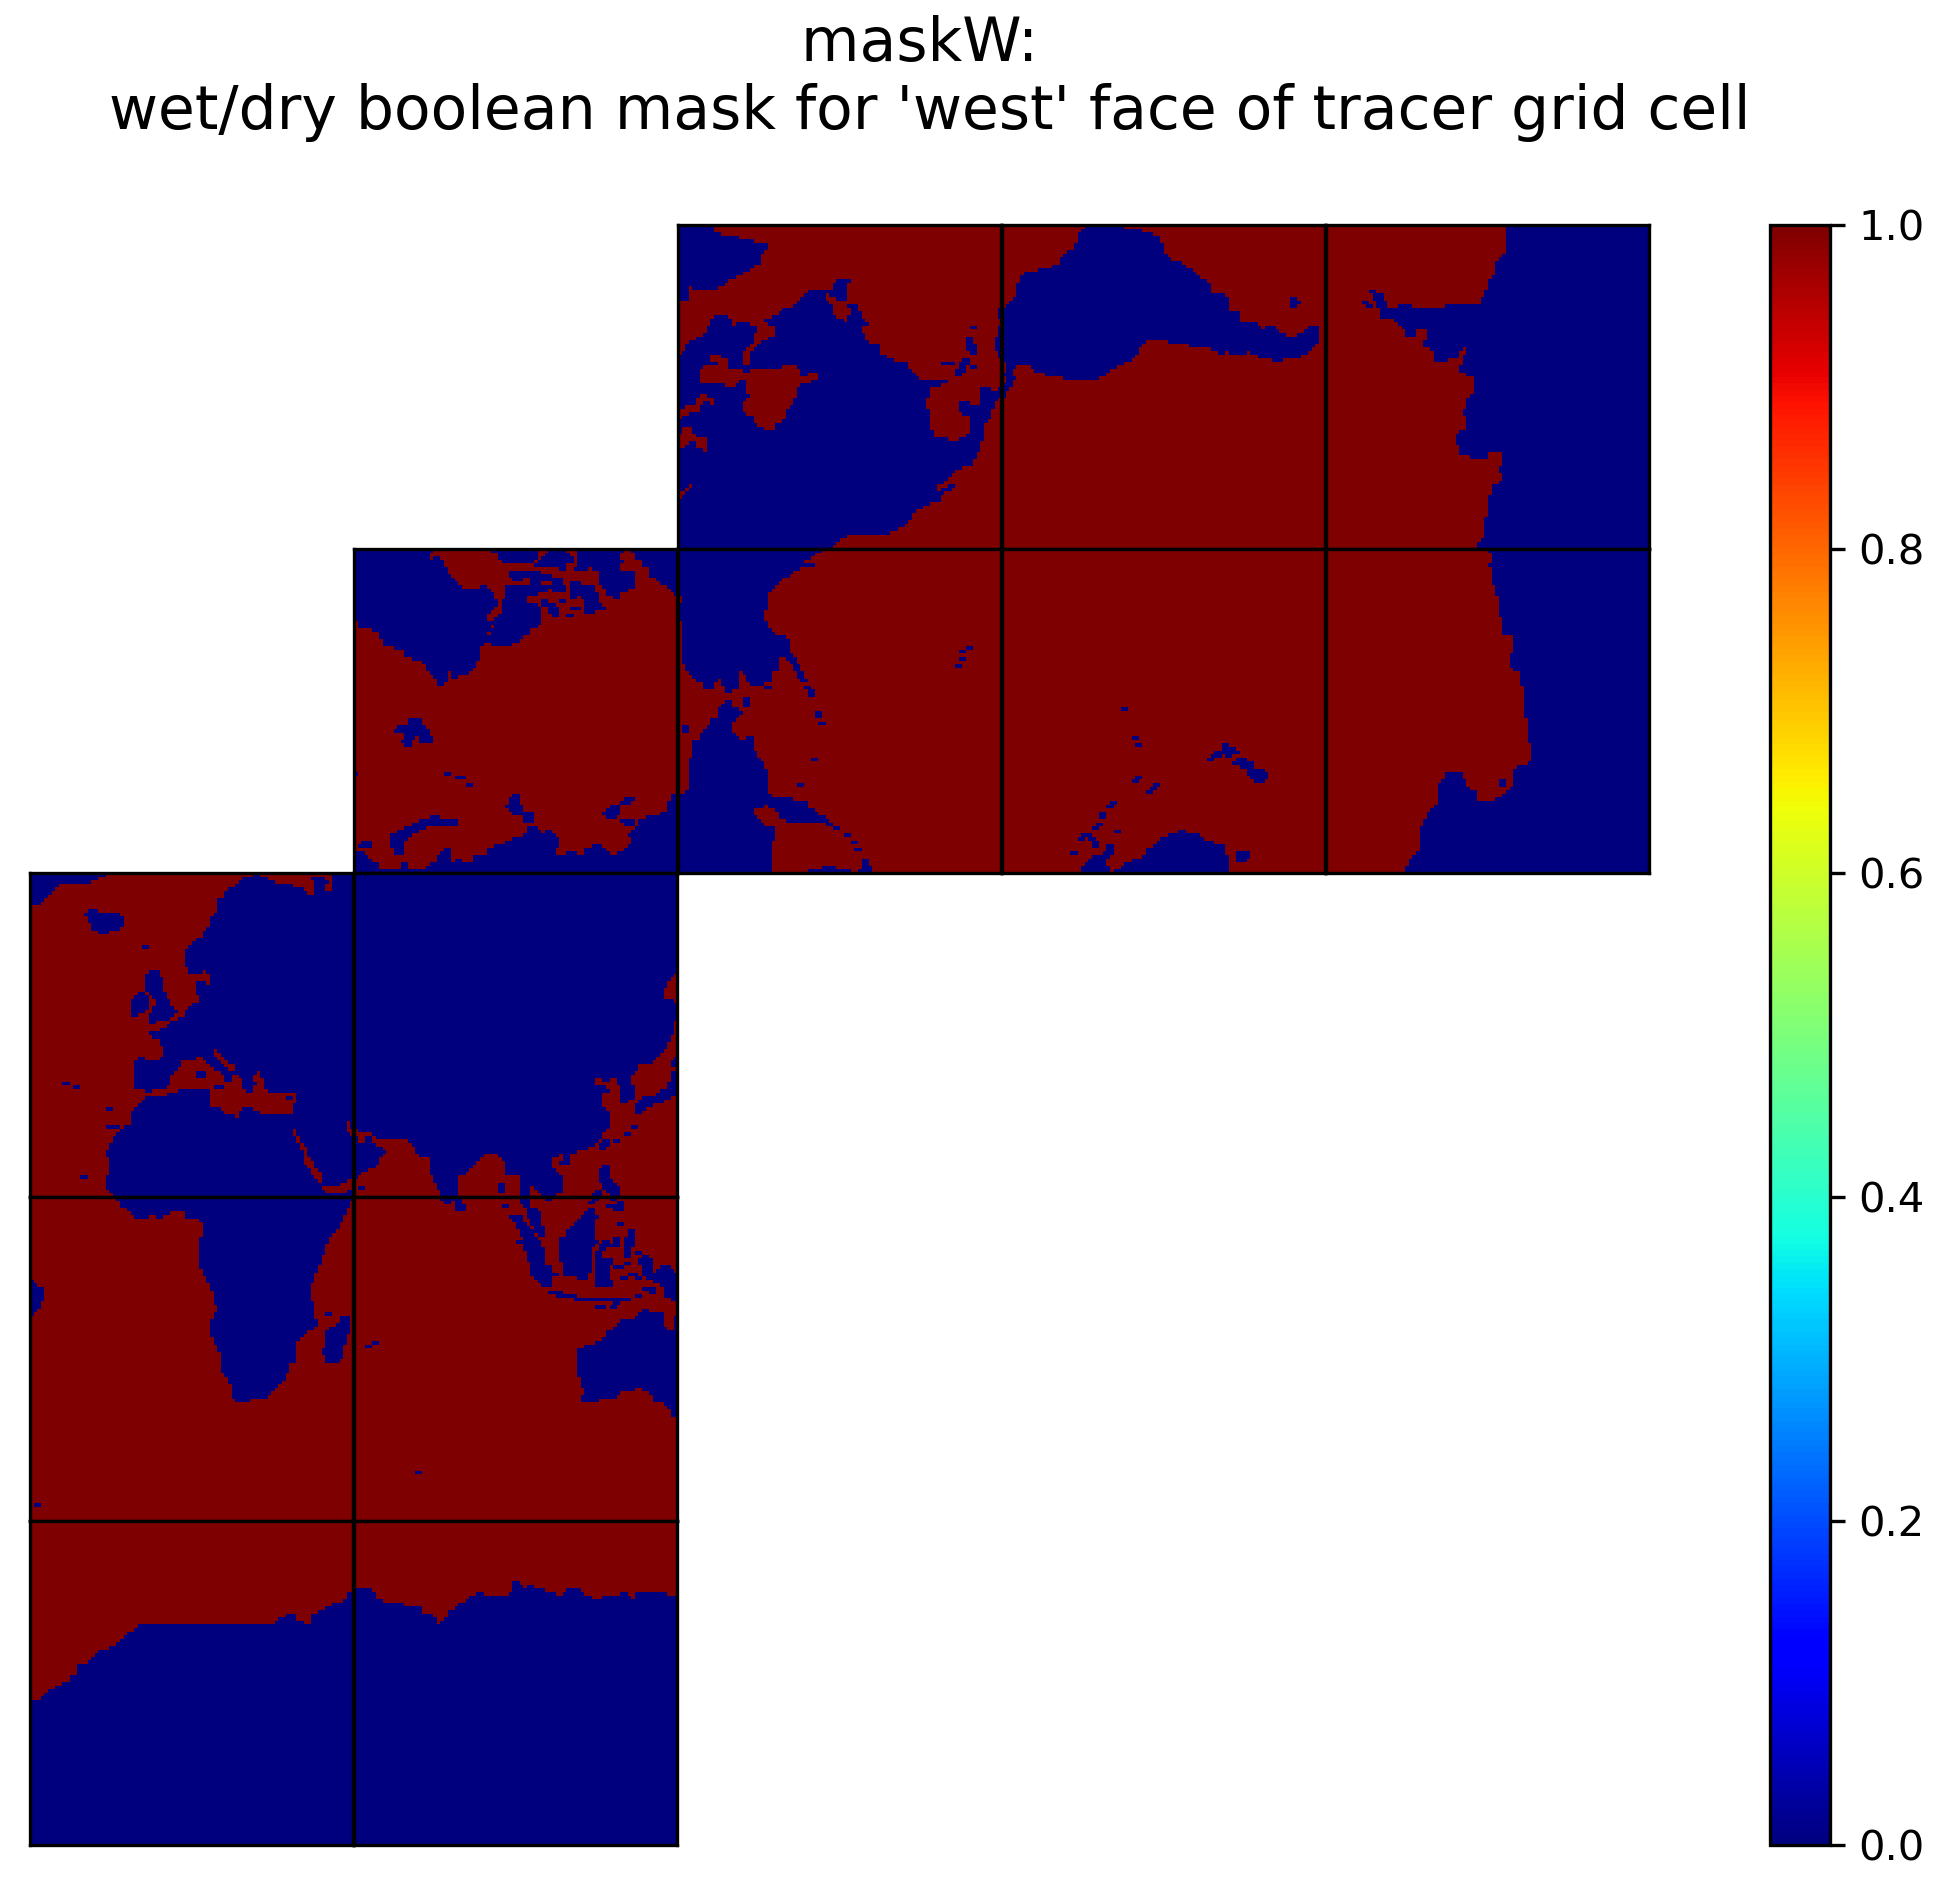
\includegraphics[scale=0.5]{../images/plots/native_plots_coords/Geometry_Parameters_for_the_Lat-Lon-Cap_90_(llc90)_Native_Model_Grid_(Version_4_Release_4)/maskW.png}
\caption{\\Dataset: GRID\_GEOMETRY\_ECCO\\Variable: maskW}
\label{tab:table-GRID_GEOMETRY_ECCO_maskW-Plot}
\end{figure}
\pagebreak
\subsubsection{Native coordinates Variable maskS}
\begin{longtable}{|p{0.06\textwidth}|p{0.41\textwidth}|p{0.39\textwidth}|p{0.06\textwidth}|}
    \caption{CDL description of GRID\_GEOMETRY\_ECCO's maskS variable}
    \label{tab:table-GRID_GEOMETRY_ECCO_maskS} \\ 
    \hline \endhead \hline \endfoot
    \rowcolor{lightgray} \textbf{Storage Type} & \textbf{Variable Name} & \textbf{Description} & \textbf{Unit} \\ \hline
    bool & maskS & wet/dry boolean mask for 'south' face of tracer grid cell & N/A \\ \hline
    \rowcolor{lightgray}  \multicolumn{4}{|p{1.00\textwidth}|}{\textbf{CDL Description}} \\ \hline
    \multicolumn{4}{|p{1.00\textwidth}|}{\makecell{\parbox{1\textwidth}{bool maskS(k, tile, j\_g, i)\\
    \hspace*{0.5cm}maskS: \_FillValue = 1\\
    \hspace*{0.5cm}maskS: long\_name = "wet/dry boolean mask for south face of tracer grid cell"\\
    \hspace*{0.5cm}maskS: coverage\_content\_type = modelResult\\
    \hspace*{0.5cm}maskS: coordinates = Z}}} \\ \hline
    \rowcolor{lightgray} \multicolumn{4}{|p{1.00\textwidth}|}{\textbf{Comments}} \\ \hline
    \multicolumn{4}{|p{1\textwidth}|}{True for grid cells with nonzero open vertical fraction along their 'south' face (hFacS > 0), otherwise False. Although hFacS can vary though time, cells will never close if starting open and will never open if starting closed: hFacS(i,j,k,t) > 0 for all t, if hFacS(i,j,k,t=0) and hFacS(i,j,k,t) = 0 for all t, if hFacS(i,j,k,t=0) = 0. Therefore, maskS is time invariant. Note: } \\ \hline
\end{longtable}

\begin{figure}[H]
\centering
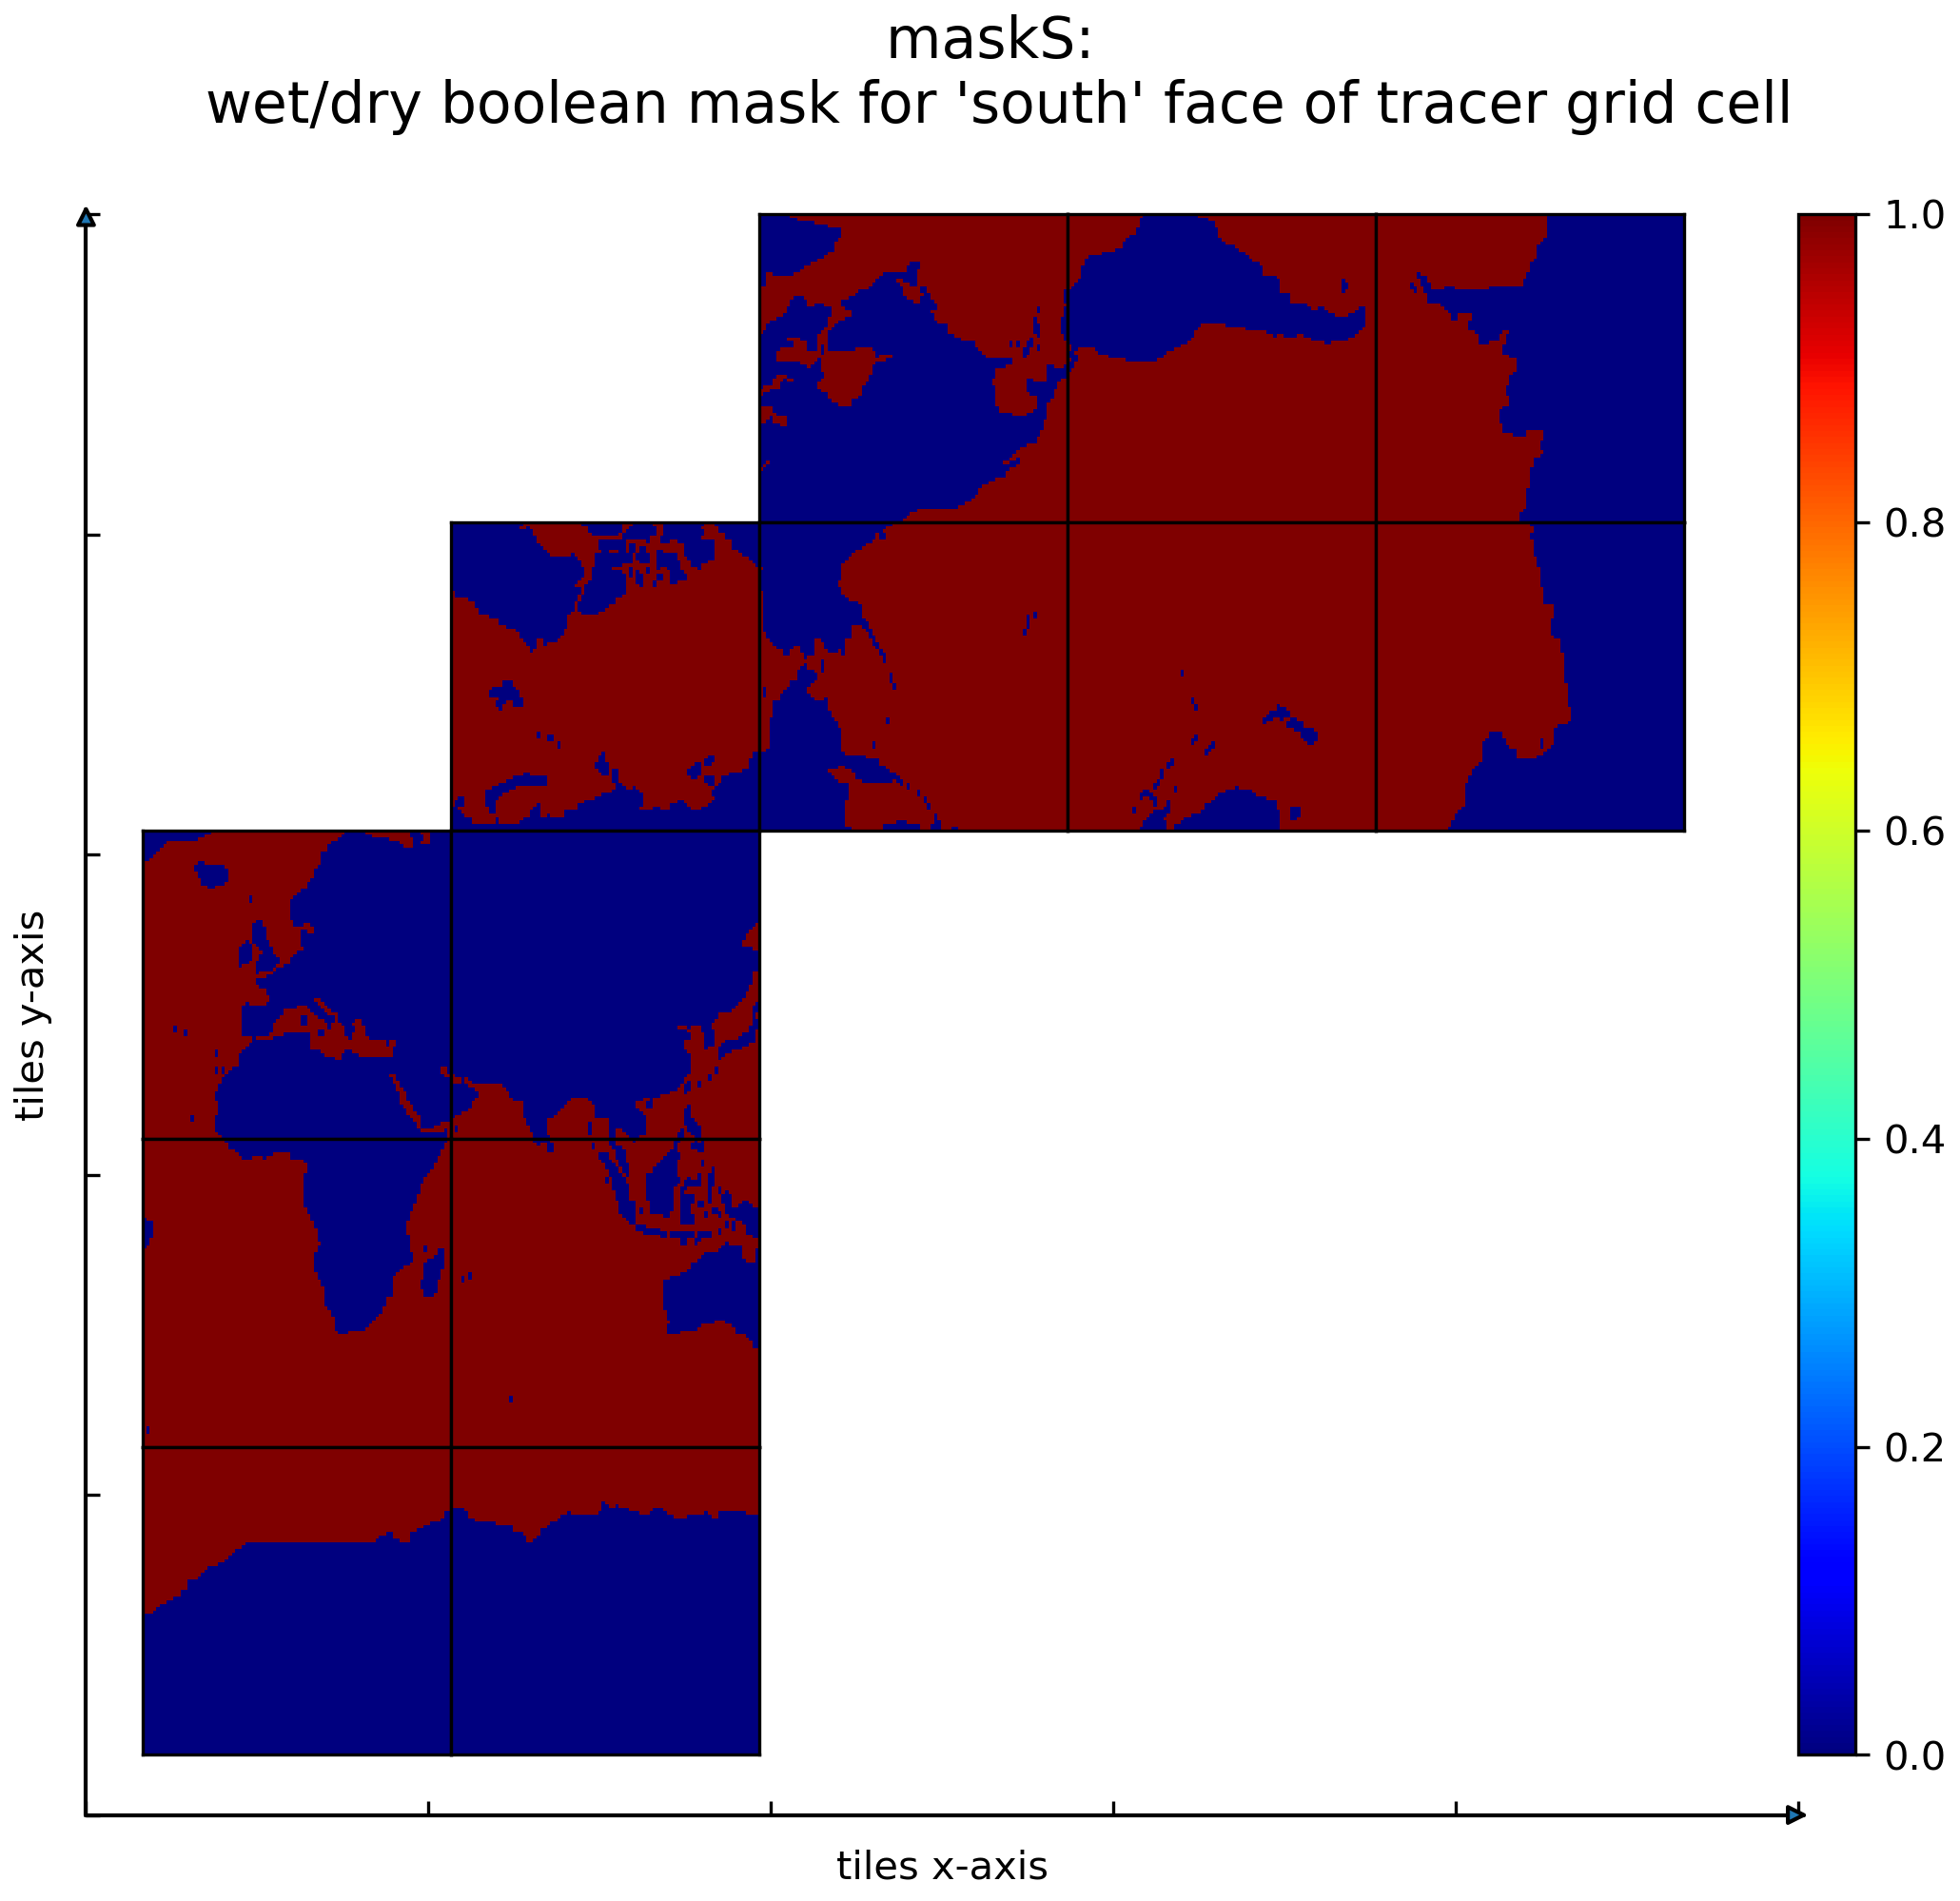
\includegraphics[scale=0.5]{../images/plots/native_plots_coords/Geometry_Parameters_for_the_Lat-Lon-Cap_90_(llc90)_Native_Model_Grid_(Version_4_Release_4)/maskS.png}
\caption{\\Dataset: GRID\_GEOMETRY\_ECCO\\Variable: maskS}
\label{tab:table-GRID_GEOMETRY_ECCO_maskS-Plot}
\end{figure}